% Options for packages loaded elsewhere
\PassOptionsToPackage{unicode}{hyperref}
\PassOptionsToPackage{hyphens}{url}
\PassOptionsToPackage{dvipsnames,svgnames*,x11names*}{xcolor}
%
\documentclass[
]{krantz}
\usepackage{lmodern}
\usepackage{amssymb,amsmath}
\usepackage{ifxetex,ifluatex}
\ifnum 0\ifxetex 1\fi\ifluatex 1\fi=0 % if pdftex
  \usepackage[T1]{fontenc}
  \usepackage[utf8]{inputenc}
  \usepackage{textcomp} % provide euro and other symbols
\else % if luatex or xetex
  \usepackage{unicode-math}
  \defaultfontfeatures{Scale=MatchLowercase}
  \defaultfontfeatures[\rmfamily]{Ligatures=TeX,Scale=1}
\fi
% Use upquote if available, for straight quotes in verbatim environments
\IfFileExists{upquote.sty}{\usepackage{upquote}}{}
\IfFileExists{microtype.sty}{% use microtype if available
  \usepackage[]{microtype}
  \UseMicrotypeSet[protrusion]{basicmath} % disable protrusion for tt fonts
}{}
\makeatletter
\@ifundefined{KOMAClassName}{% if non-KOMA class
  \IfFileExists{parskip.sty}{%
    \usepackage{parskip}
  }{% else
    \setlength{\parindent}{0pt}
    \setlength{\parskip}{6pt plus 2pt minus 1pt}}
}{% if KOMA class
  \KOMAoptions{parskip=half}}
\makeatother
\usepackage{xcolor}
\IfFileExists{xurl.sty}{\usepackage{xurl}}{} % add URL line breaks if available
\IfFileExists{bookmark.sty}{\usepackage{bookmark}}{\usepackage{hyperref}}
\hypersetup{
  pdftitle={Data Disasters},
  pdfauthor={Emily Riederer},
  colorlinks=true,
  linkcolor=Maroon,
  filecolor=Maroon,
  citecolor=Blue,
  urlcolor=Blue,
  pdfcreator={LaTeX via pandoc}}
\urlstyle{same} % disable monospaced font for URLs
\usepackage{color}
\usepackage{fancyvrb}
\newcommand{\VerbBar}{|}
\newcommand{\VERB}{\Verb[commandchars=\\\{\}]}
\DefineVerbatimEnvironment{Highlighting}{Verbatim}{commandchars=\\\{\}}
% Add ',fontsize=\small' for more characters per line
\usepackage{framed}
\definecolor{shadecolor}{RGB}{248,248,248}
\newenvironment{Shaded}{\begin{snugshade}}{\end{snugshade}}
\newcommand{\AlertTok}[1]{\textcolor[rgb]{0.33,0.33,0.33}{#1}}
\newcommand{\AnnotationTok}[1]{\textcolor[rgb]{0.37,0.37,0.37}{\textbf{\textit{#1}}}}
\newcommand{\AttributeTok}[1]{\textcolor[rgb]{0.61,0.61,0.61}{#1}}
\newcommand{\BaseNTok}[1]{\textcolor[rgb]{0.06,0.06,0.06}{#1}}
\newcommand{\BuiltInTok}[1]{#1}
\newcommand{\CharTok}[1]{\textcolor[rgb]{0.5,0.5,0.5}{#1}}
\newcommand{\CommentTok}[1]{\textcolor[rgb]{0.37,0.37,0.37}{\textit{#1}}}
\newcommand{\CommentVarTok}[1]{\textcolor[rgb]{0.37,0.37,0.37}{\textbf{\textit{#1}}}}
\newcommand{\ConstantTok}[1]{\textcolor[rgb]{0,0,0}{#1}}
\newcommand{\ControlFlowTok}[1]{\textcolor[rgb]{0.27,0.27,0.27}{\textbf{#1}}}
\newcommand{\DataTypeTok}[1]{\textcolor[rgb]{0.27,0.27,0.27}{#1}}
\newcommand{\DecValTok}[1]{\textcolor[rgb]{0.06,0.06,0.06}{#1}}
\newcommand{\DocumentationTok}[1]{\textcolor[rgb]{0.37,0.37,0.37}{\textbf{\textit{#1}}}}
\newcommand{\ErrorTok}[1]{\textcolor[rgb]{0.14,0.14,0.14}{\textbf{#1}}}
\newcommand{\ExtensionTok}[1]{#1}
\newcommand{\FloatTok}[1]{\textcolor[rgb]{0.06,0.06,0.06}{#1}}
\newcommand{\FunctionTok}[1]{\textcolor[rgb]{0,0,0}{#1}}
\newcommand{\ImportTok}[1]{#1}
\newcommand{\InformationTok}[1]{\textcolor[rgb]{0.37,0.37,0.37}{\textbf{\textit{#1}}}}
\newcommand{\KeywordTok}[1]{\textcolor[rgb]{0.27,0.27,0.27}{\textbf{#1}}}
\newcommand{\NormalTok}[1]{#1}
\newcommand{\OperatorTok}[1]{\textcolor[rgb]{0.43,0.43,0.43}{\textbf{#1}}}
\newcommand{\OtherTok}[1]{\textcolor[rgb]{0.37,0.37,0.37}{#1}}
\newcommand{\PreprocessorTok}[1]{\textcolor[rgb]{0.37,0.37,0.37}{\textit{#1}}}
\newcommand{\RegionMarkerTok}[1]{#1}
\newcommand{\SpecialCharTok}[1]{\textcolor[rgb]{0,0,0}{#1}}
\newcommand{\SpecialStringTok}[1]{\textcolor[rgb]{0.5,0.5,0.5}{#1}}
\newcommand{\StringTok}[1]{\textcolor[rgb]{0.5,0.5,0.5}{#1}}
\newcommand{\VariableTok}[1]{\textcolor[rgb]{0,0,0}{#1}}
\newcommand{\VerbatimStringTok}[1]{\textcolor[rgb]{0.5,0.5,0.5}{#1}}
\newcommand{\WarningTok}[1]{\textcolor[rgb]{0.37,0.37,0.37}{\textbf{\textit{#1}}}}
\usepackage{longtable,booktabs}
% Correct order of tables after \paragraph or \subparagraph
\usepackage{etoolbox}
\makeatletter
\patchcmd\longtable{\par}{\if@noskipsec\mbox{}\fi\par}{}{}
\makeatother
% Allow footnotes in longtable head/foot
\IfFileExists{footnotehyper.sty}{\usepackage{footnotehyper}}{\usepackage{footnote}}
\makesavenoteenv{longtable}
\usepackage{graphicx}
\makeatletter
\def\maxwidth{\ifdim\Gin@nat@width>\linewidth\linewidth\else\Gin@nat@width\fi}
\def\maxheight{\ifdim\Gin@nat@height>\textheight\textheight\else\Gin@nat@height\fi}
\makeatother
% Scale images if necessary, so that they will not overflow the page
% margins by default, and it is still possible to overwrite the defaults
% using explicit options in \includegraphics[width, height, ...]{}
\setkeys{Gin}{width=\maxwidth,height=\maxheight,keepaspectratio}
% Set default figure placement to htbp
\makeatletter
\def\fps@figure{htbp}
\makeatother
\setlength{\emergencystretch}{3em} % prevent overfull lines
\providecommand{\tightlist}{%
  \setlength{\itemsep}{0pt}\setlength{\parskip}{0pt}}
\setcounter{secnumdepth}{5}
\usepackage{booktabs}
\usepackage{longtable}
\usepackage[bf,singlelinecheck=off]{caption}

\usepackage{framed,color}
\definecolor{shadecolor}{RGB}{248,248,248}

\renewcommand{\textfraction}{0.05}
\renewcommand{\topfraction}{0.8}
\renewcommand{\bottomfraction}{0.8}
\renewcommand{\floatpagefraction}{0.75}

\renewenvironment{quote}{\begin{VF}}{\end{VF}}
\let\oldhref\href
\renewcommand{\href}[2]{#2\footnote{\url{#1}}}

\makeatletter
\newenvironment{kframe}{%
\medskip{}
\setlength{\fboxsep}{.8em}
 \def\at@end@of@kframe{}%
 \ifinner\ifhmode%
  \def\at@end@of@kframe{\end{minipage}}%
  \begin{minipage}{\columnwidth}%
 \fi\fi%
 \def\FrameCommand##1{\hskip\@totalleftmargin \hskip-\fboxsep
 \colorbox{shadecolor}{##1}\hskip-\fboxsep
     % There is no \\@totalrightmargin, so:
     \hskip-\linewidth \hskip-\@totalleftmargin \hskip\columnwidth}%
 \MakeFramed {\advance\hsize-\width
   \@totalleftmargin\z@ \linewidth\hsize
   \@setminipage}}%
 {\par\unskip\endMakeFramed%
 \at@end@of@kframe}
\makeatother

\renewenvironment{Shaded}{\begin{kframe}}{\end{kframe}}

\usepackage{makeidx}
\makeindex

\urlstyle{tt}

\usepackage{amsthm}
\makeatletter
\def\thm@space@setup{%
  \thm@preskip=8pt plus 2pt minus 4pt
  \thm@postskip=\thm@preskip
}
\makeatother

\frontmatter
\ifluatex
  \usepackage{selnolig}  % disable illegal ligatures
\fi
\usepackage[]{natbib}
\bibliographystyle{apalike}

\title{Data Disasters}
\author{Emily Riederer}
\date{2021-08-03}

\begin{document}
\maketitle

% you may need to leave a few empty pages before the dedication page

%\cleardoublepage\newpage\thispagestyle{empty}\null
%\cleardoublepage\newpage\thispagestyle{empty}\null
%\cleardoublepage\newpage
\thispagestyle{empty}

\begin{center}
To all the mistakes I've made (data, and otherwise) and those who tolerated my making them.
%\includegraphics{images/dedication.pdf}
\end{center}

\setlength{\abovedisplayskip}{-5pt}
\setlength{\abovedisplayshortskip}{-5pt}

{
\hypersetup{linkcolor=}
\setcounter{tocdepth}{2}
\tableofcontents
}
\listoftables
\listoffigures
\hypertarget{preface}{%
\chapter*{Preface}\label{preface}}


\begin{center}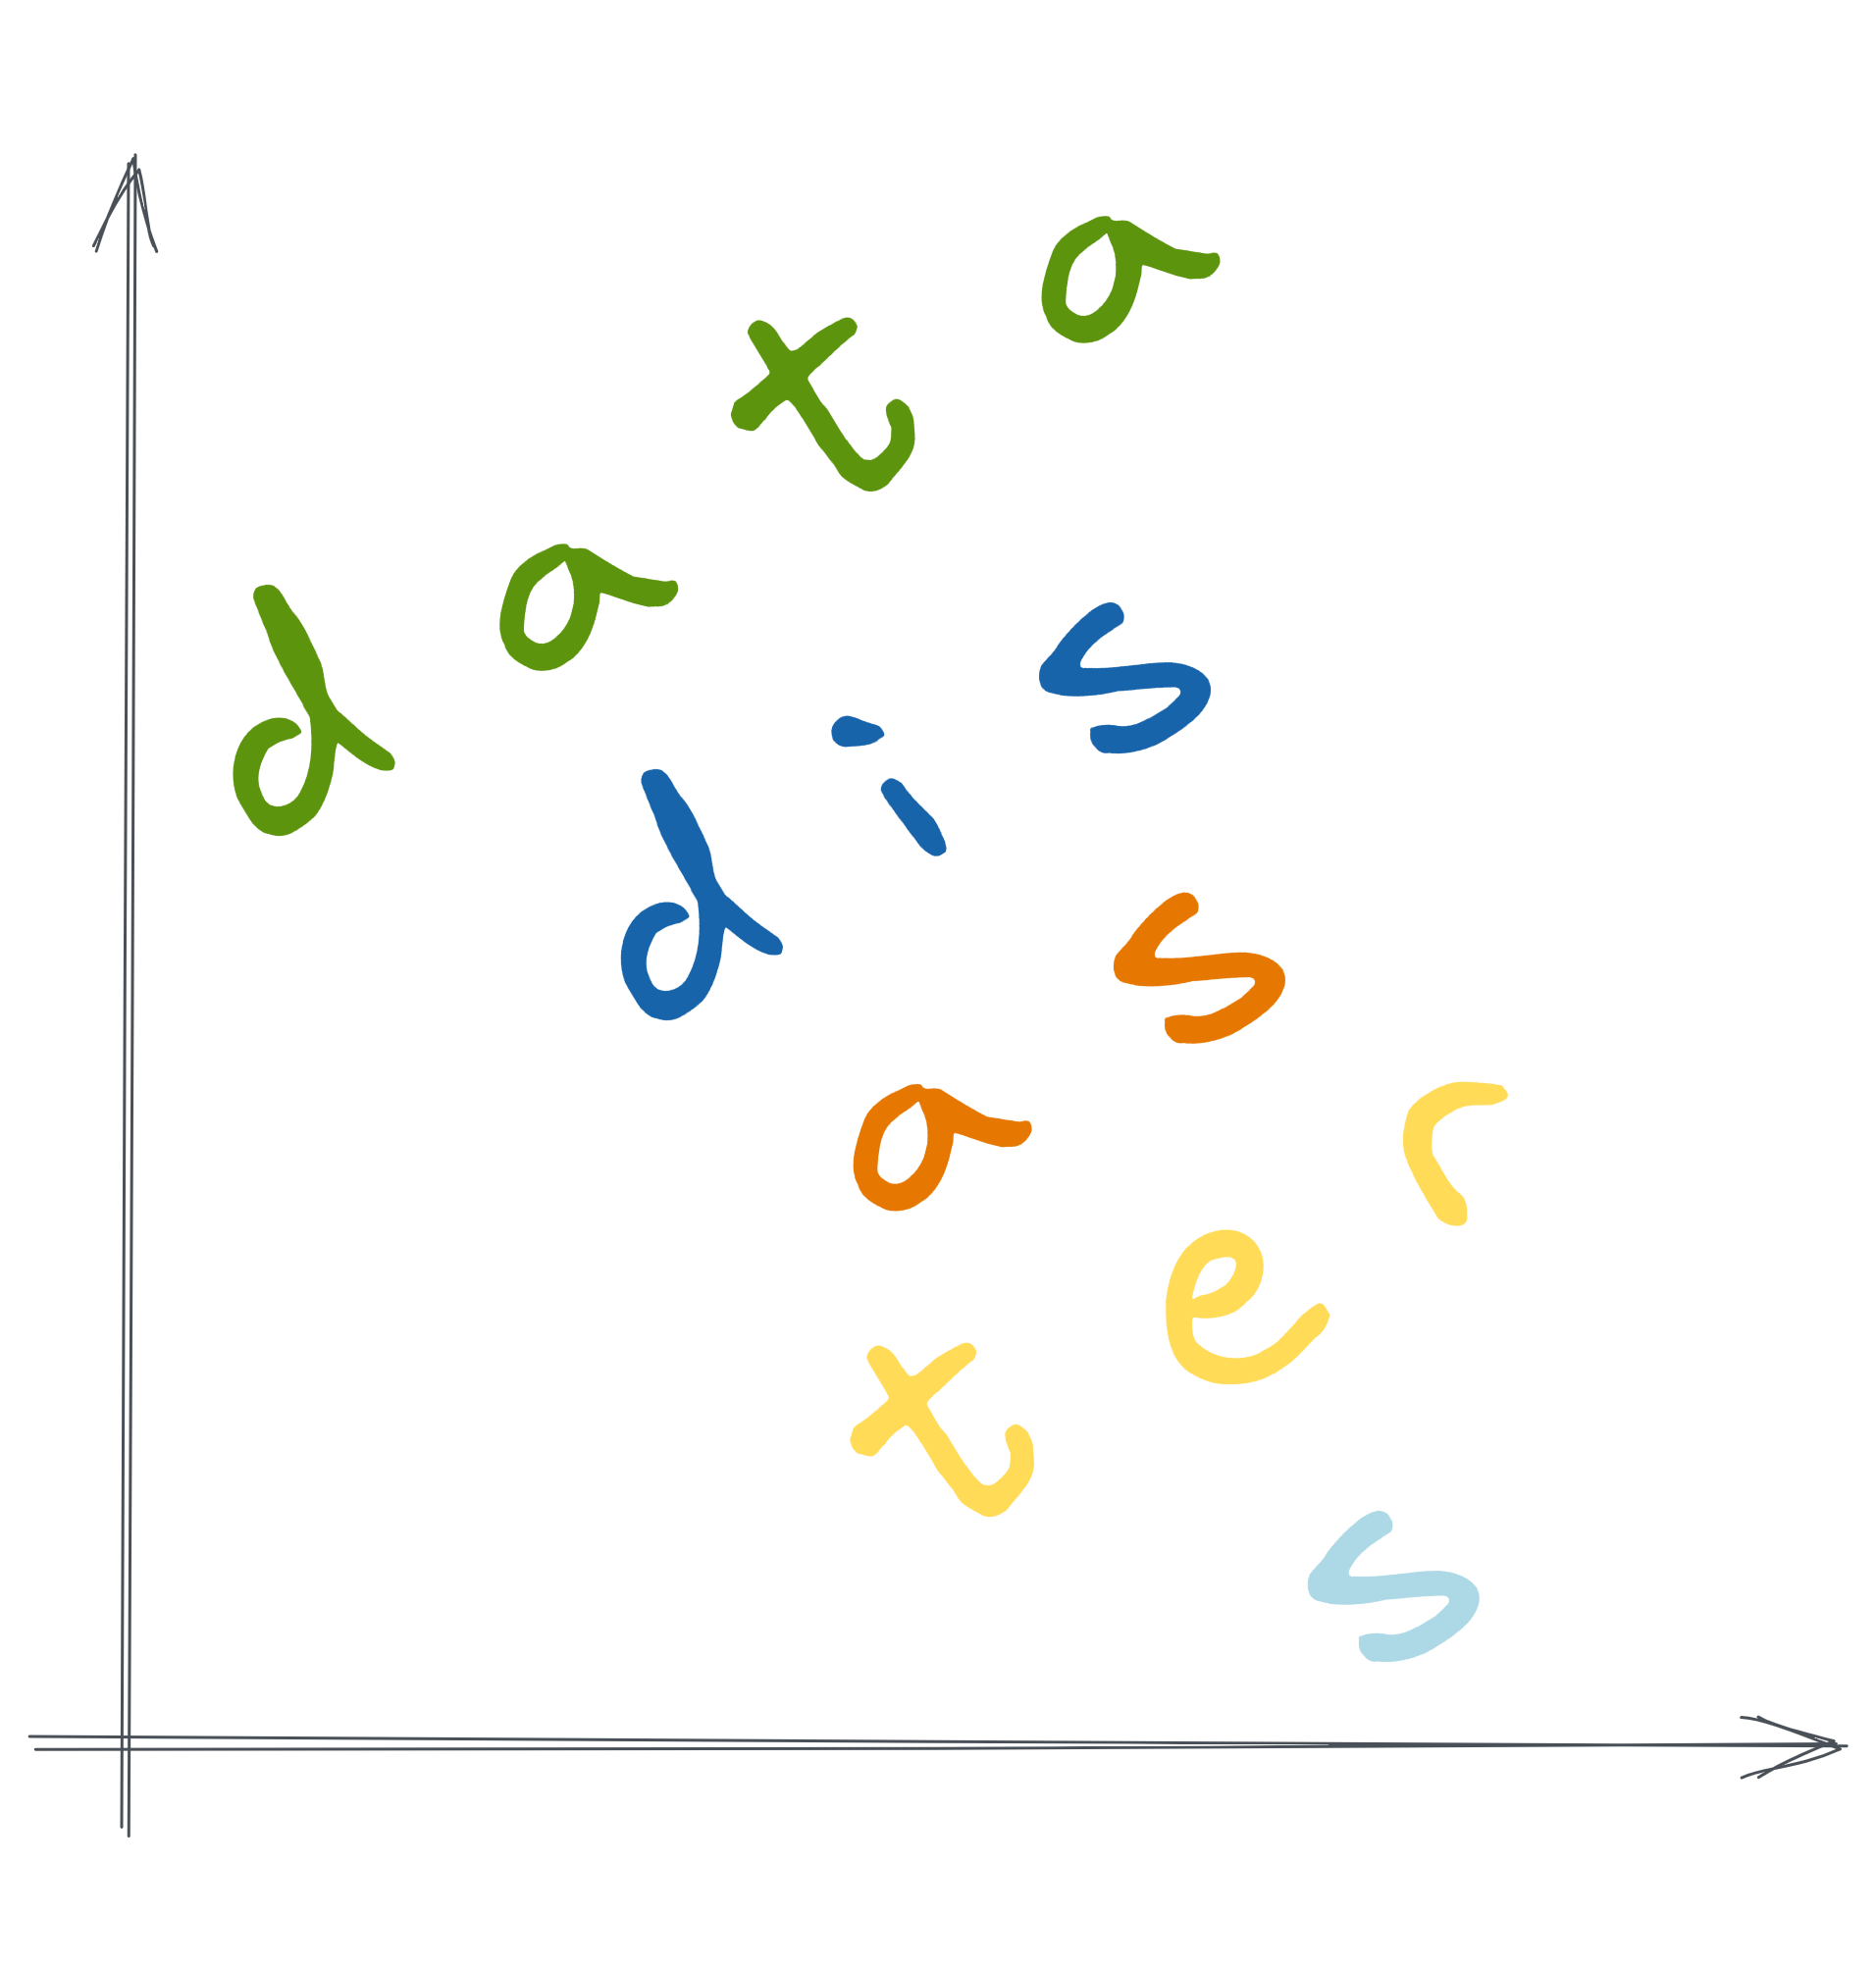
\includegraphics[width=0.9\linewidth]{figures/cover} \end{center}

Training in data analysis often begins with Statistics 101 course.
Students learn the ``happy path'' of answer data that adheres to specific assumptions (such as ``independent and identically distributed with a Normal density'') and answers pre-specified questions (most notably, the infamous null hypothesis significance test).
Then, they venture out into the world of real-world data analysis where non-experimental data is rarely so well behaved and the questions asked of it are far more nuanced.

No one course should aim to teach students everything they should know about statistics.
In fact, one of the best parts about a career in statistics is the responsibility and privilege of life-long learning.
However, \textbf{the flaw of introductory statistics is not that it's incomplete, but that it's not obvious how it is \emph{not} complete}.
Statistics is a bad salesman.
There's no season finale, no cliff hanger, no teasing and hinting and promising more and better to come.
Student may leave their studies believing that answering more complex data analysis questions is trivially easy (by relying on the one-size-fits-all ``panacea'' that they learned) or intractably difficult (when the assumptions of that method are not met.)

This book attempts to add more color to all the dimensions of data analysis while showcasing the nuances throughout the true \emph{life cycle} of data analysis using two strategies.

First, it attempts to highlight common pitfalls in all the parts of data analysis: from data management and computation to visualization, interpretation, and modeling and even to communication and collaboration.
Data analysis is fundamentally a \emph{creative} task, so there are rarely canonical one-size-fits-all solutions.
Curiously, however, there are plenty of canonical \emph{issues} even if they require different solutions in different settings.
Thus, the goal of this book is to highlight common \emph{data disasters} and, in doing so, help students cultivate an intuition for how to detect common problems before they occur in an important analysis.

Second, while exploring these \emph{data disasters}, we humbly put forth a (woefully incomplete!) literature review of more advanced methods from statistics and other quantitative disciplines (e.g.~economics, epidemiology), to help learners build a ``mental index'' of terms to search and techniques to study should they encounter a relevant problem.

\hypertarget{main-topics}{%
\section{Main Topics}\label{main-topics}}

In particular, we will aim to help you avoid eleven types of data disasters:

\begin{itemize}
\tightlist
\item
  \textbf{Data Dalliances}: Misinterpreting or misuing data based on how it was collected or what it represents
\item
  \textbf{Computational Quandaries}: Letting computers do what you said and not what you meant
\item
  \textbf{Egregious Aggregations}: Losing critical information when information is condensed
\item
  \textbf{Vexing Visualization}: Confusing ourselves or others with plotting choices
\item
  \textbf{Incredible Inferences}: Drawing incorrect conclusions for analytical results
\item
  \textbf{Cavalier Causality}: Falling prey to spurious correlations masquerading as causality
\item
  \textbf{Mindless Modeling}: Failing to get the most value out of models by not tailoring the features, targets, and performance metrics
\item
  \textbf{Alternative Algorithms}: Lacking an understanding of alternative methods which may be better suited for the problem at hand
\item
  \textbf{Futile Findings}: Asking and answering questions that aren't useful
\item
  \textbf{Complexifying Code}: Making projects unwieldy or more difficult to understand than necessary
\item
  \textbf{Rejecting Reproducibility}: Working inefficiently instead of an efficient, reproducible, and sharable workflow
\end{itemize}

\hypertarget{common-themes}{%
\section{Common Themes}\label{common-themes}}

In each chapter, we will see numerous examples of each disaster and consider strategies to help us mitigate.
Along the way, we'll emphasize:

\begin{itemize}
\tightlist
\item
  The importance of \textbf{domain knowledge} and the \textbf{data-generating process} to decide what it is you want to do
\item
  The utility of \textbf{simulation} as a tool to explore if, in fact, you are doing it
\item
  The exploration of \textbf{counterexamples} to build \textbf{intuition for common patterns} of problems even where common solutions don't exist
\end{itemize}

As we go, we will notice how three common themes that challenge the focus of introductory statistics:

\begin{itemize}
\tightlist
\item
  Summary statistics mask interesting stories that we see when focusing on the \textbf{variation}
\item
  Similarly, observations and variables are rarely independent; the story is in the \textbf{covariance}
\item
  Assumptions of Normality, or more broadly symmetry, are often in appropriate in wonky, \textbf{highly skewed} world
\end{itemize}

\hypertarget{about-the-author}{%
\chapter*{About the Author}\label{about-the-author}}


\textbf{Emily Riederer} is\ldots{}

Find me on my \href{https://emilyriederer.netlify.com?utm_source=datadisasters}{website} and on \href{https://twitter.com/EmilyRiederer}{Twitter}

\mainmatter

\hypertarget{introduction-todo}{%
\chapter{Introduction (TODO)}\label{introduction-todo}}

Statistics is not synonymous with data analysis; rigor vs practicality

``Evaluating the Success of a Data Analysis'' \citep{hicks2019evaluating}

``Data Alone is not Ground Truth'' \citep{bassa_2017}

\hypertarget{what-is-data}{%
\section{What is data?}\label{what-is-data}}

Data is\ldots{}

\hypertarget{what-is-analysis}{%
\section{What is analysis?}\label{what-is-analysis}}

Analysis is the process of turning information into insight\ldots S

\hypertarget{what-is-workflow}{%
\section{What is workflow?}\label{what-is-workflow}}

Workflows are an intentional process for accomplishing a complex goal\ldots{}

\hypertarget{what-is-data-analysis}{%
\section{What is data analysis?}\label{what-is-data-analysis}}

Data analysis altogether is\ldots{}

\hypertarget{what-are-data-disasters}{%
\section{What are data disasters?}\label{what-are-data-disasters}}

Data disasters occur when\ldots{}

\hypertarget{part-data}{%
\part*{Data}\label{part-data}}


\hypertarget{data-dall}{%
\chapter{Data Dalliances (WIP)}\label{data-dall}}

The first step to data analysis is, in fact, data. While this may seem obvious, statistics textbooks often dodge this detail.
Discussions of regression analysis often begin with a statement like:

\begin{quote}
``Let \(X\) be the \(n x p\) design matrix of independent variables\ldots{}''
\end{quote}

but in practice this statement is as absurd as writing a book about how to win a basketball game, assuming your team already has a 20 point lead with 1 minute left to play.

It's very convenient but typically incorrect to assume that the data we happen to have is the ideal (or, more humbly, sufficient) data for the questions we wish to analyze.
The specific vagaries of data vary greatly by domain, but a commonality across many fields (such as political science, economics, epidemiology, and market research) is that we are often called to work with \emph{found data} (or, more formally, ``observational data'') from administrative sources or production systems.
In contrast to artisanally crafted data experimental data (like the carefully controlled agricultural experiments which motivated many early methods developments in statistics), this data was generated neither by us not for us.
To quote Angela Bassa, the head of data science at an e-commerce company: ``Data isn't ground truth. Data are artifacts of systems'' \citep{bassa_2017}.

The analytical implications of observational versus experimental data are well explored in the field of causal inference (which we will discuss some in Chapters \ref{incr-infe} and \ref{cava-caus}).
However, this distinction has implications far earlier in the data analysis process, as well.
To name a few:

\begin{itemize}
\tightlist
\item
  Records and fields many not represent the entities or measures most conducive to analysis
\item
  Data collection methods may capture a different subset of events or do so at a different frequency than we expected, leading to systemic biases
\item
  Data movement between systems can insert errors (or, at minimum, challenges to our intuition)
\item
  Data transformations may be fragile or transient, reflecting the primary purpose of the system not our unrelated analytical use
\end{itemize}

In this chapter, we will explore data structures and the full data generating process to better understand how different types of data challenges emerge.
In doing so, we will hone sharper intuition for how our data can deceive us and what to watch out for when beginning an analysis.

\hypertarget{preliminaries}{%
\section{Preliminaries}\label{preliminaries}}

Before we begin our exploration of data dalliances, we must first establish a baseline understanding of data structure, data production, and data quality.

\hypertarget{data-structure-basics}{%
\subsection{Data Structure Basics}\label{data-structure-basics}}

\hypertarget{relational-data-structure}{%
\subsubsection{Relational Data Structure}\label{relational-data-structure}}

Understanding the content and structure of the data you are using is a critical prerequisite to analysis.
In this book, we focus on tabular, structured data like one might find in an Excel spreadsheet or relational database.\footnote{Other types of data that one might encounter in the wild include free text, JSON, spatial data, and more. However, many of these require either more advanced analysis techniques or structuring that converts them into tabular data, so they are out of the scope of this discussion.}

In particular, many tools work best with what R developer Hadley Wickham describes as ``tidy data'' \citep{wickham_tidy}. Namely:

\begin{enumerate}
\def\labelenumi{\arabic{enumi}.}
\tightlist
\item
  Each variable forms a column
\item
  Each observation forms a row
\item
  Each type of observational unit forms a table
\end{enumerate}

This is analogous to how one generally finds data arranged in a database and how statisticians are used to conceptualizing it.
For example, the design matrix of a linear model consists of one column of data for each independent variable to be included in the model and one row for each observation.\footnote{When data is arrange this way in a matrix \(X\), linear regression coefficients can be computed as \(\beta = (\mathbf{X}^\intercal\mathbf{X})^{-1}\mathbf{X}^\intercal \mathbf{y}\)}
As Wickham points out, this is also similar to what is called ``3rd normal form'' in the world of relational database management systems.

Using this data structure is valuable not only because it is similar to what many modern data tools expect, but also because it provides us a framework to think critically about what defined each observation and each variable in our dataset.

\hypertarget{schemas-todo}{%
\subsubsection{Schemas (TODO)}\label{schemas-todo}}

\hypertarget{data-production-processes}{%
\subsection{Data Production Processes}\label{data-production-processes}}

In statistical modeling we discuss the \textbf{data generating process}: we can build models that describe the mechanisms that create our observations.
We can broaden this notion to think about the generating process of each of these steps of data production.

Regardless of the type of data (experimental, observational, survey, etc.), there are generally four main steps to production: collection, extraction, loading, and transformation.\footnote{You may hear the last three referred to as ELT or ETL}

\begin{itemize}
\tightlist
\item
  \textbf{Collect}: The way in which signals from the real world are captured as data. This could include logging (e.g.~for web traffic or system monitoring), sensors (e.g.~temperature collection), surveys, and more
\item
  \textbf{Extract}: The process of removing data from the place in which it was originally captured in preparation of moving it somewhere in which analysis can be done
\item
  \textbf{Load}: The process of loading the extracted data to its final destination
\item
  \textbf{Transform}: The process of modeling and transforming data so that its structure is useful for analysis and its variables are interpretable
\end{itemize}

To better theorize about data quality issues, it's useful to think of four DGPs (as shown in Figure \ref{fig:dgp}): the real-world DGP, the data collection/extraction DGP\footnote{I don't mean to imply statisticians do not regularly think about the data collection DGP! The rich literature on missing data imputation, censored data in survival analysis, and non-response bias is survey data collection are just a few examples of how carefully statisticians think about how data collection impacts analysis. I chose to break it out here to discuss the more technical aspects of collection}, the data loading DGP, and the data transformation DGP.

\begin{figure}

{\centering 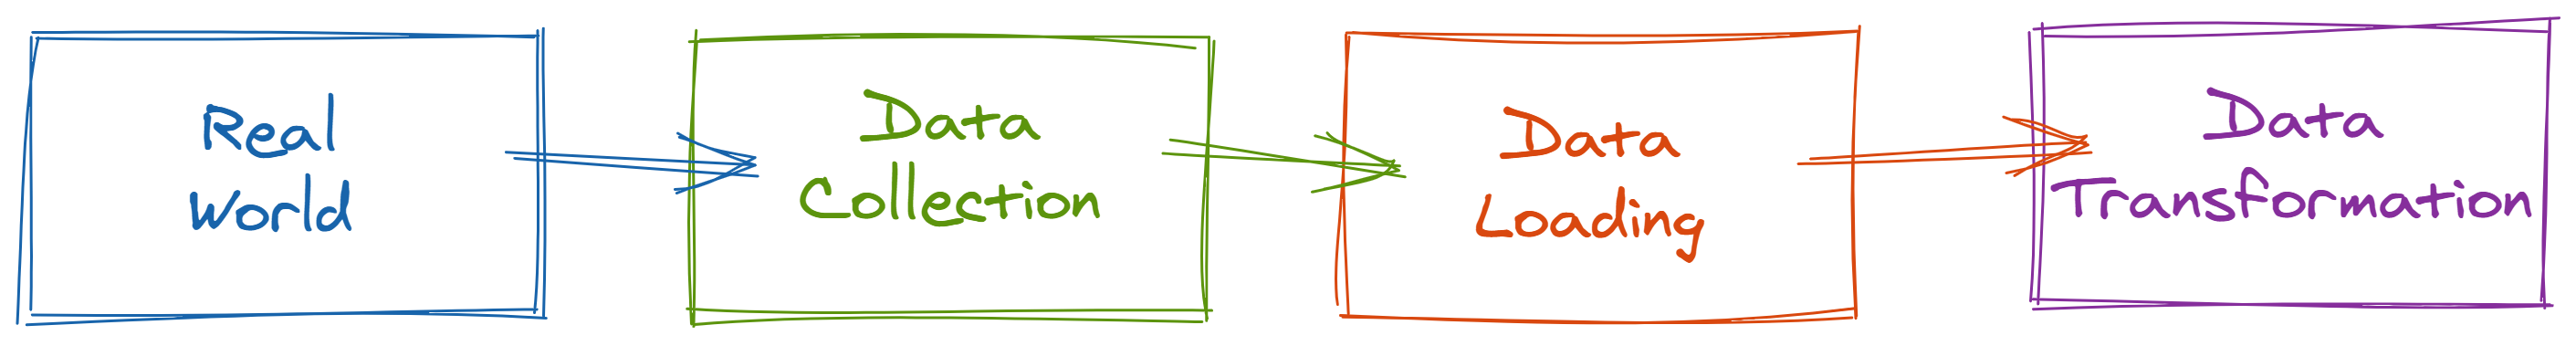
\includegraphics[width=0.9\linewidth]{figures/data-dall/dgp} 

}

\caption{A schematic of the data production process}\label{fig:dgp}
\end{figure}

\hypertarget{e-commerce-data-example}{%
\subsubsection{E-Commerce Data Example}\label{e-commerce-data-example}}

For example, consider the role of each of these four DGPs for e-commerce data:

\begin{itemize}
\tightlist
\item
  \textbf{Real-world DGP}: Supply, demand, marketing, and a range of factors motivate a consumer to visit a website and make a purchase
\item
  \textbf{Data collection DGP}: Parts of the website are instrumented to log certain customer actions. This log is then extracted from the different operational system (login platforms, payment platforms, account records) to be used for analysis
\item
  \textbf{Data loading DGP}: Data recorded by different systems is moved to a data warehouse for further processing through some sort of manual, scheduled, or orchestrated job. These different systems may make data available at different frequencies.
\item
  \textbf{Data transformation DGP}: To arrive at that final data presentation requires creating a \href{https://en.wikipedia.org/wiki/Data_model}{data model} to describe domain-specific attributes with key variables crafted with data transformations
\end{itemize}

\hypertarget{subway-data-example}{%
\subsubsection{Subway Data Example}\label{subway-data-example}}

Or, consider the role of each of these four DGPs for subway ridership data\footnote{Like NYC's infamously messy \href{http://web.mta.info/developers/turnstile.html}{turnstile data}. I don't claim to know precisely how this dataset is created, but many of the specific challenges it contains are highly relevant.}:

\begin{itemize}
\tightlist
\item
  \textbf{Real-world DGP}: Riders are motivated to use public transportation to commute, run errands, or visit friends. Different motivating factors may cause different weekly and annual seasonality
\item
  \textbf{Data collection DGP}: To ride the subway, riders go to a station and enter and exit through turnstiles. The mechanical rotation of the turnstile caused by a rider passing through is recorded
\item
  \textbf{Data loading DGP}: Data recorded at each turnstile is collected through a centralized computer system at the station. Once a week, each station uploads a flat file of this data to a data lake owned by the city's Department of Transportation
\item
  \textbf{Data transformation DGP}: Turnstiles from different companies may have different data formats. Transformation may include harmonizing disparate sources, coding system-generated codes (e.g.~Station XYZ) to semantically meaningful names (e.g.~Main Street Station), and publishing a final unified representation across stations and across time
\end{itemize}

Throughout this chapter, we'll explore how understanding key concepts about each of these DGPs can help guide our intuition on where to look for problems.

\hypertarget{data-quality-dimension}{%
\subsection{Data Quality Dimension}\label{data-quality-dimension}}

To guide our discussion of how data production can affect aspects of data quality, we need a guiding definition of data quality.
This is challenging because data quality is \emph{subjective} and \emph{task-specific}.
It matters much more if data is ``fit for purpose'' and operates in a way that is \emph{transparent} to its users moreso than meeting some preordained quality standard.

Regardless, it's useful for our discussion to think about general dimensions of data quality. Here, we will rely on six dimensions of data quality outlined by Data Management Association \citep{dama}.
Their official definitions are:

\begin{enumerate}
\def\labelenumi{\arabic{enumi}.}
\tightlist
\item
  \textbf{Completeness}: The proportion of stored data against the potential of ``100\% complete''
\item
  \textbf{Uniqueness}: Nothing will be recorded more than once based upon how that thing is identified. It is the inverse of an assessment of the level of duplication
\item
  \textbf{Timeliness}: The degree to which data represent reality from the required point in time
\item
  \textbf{Validity}: Data are valid if it conforms to the syntax (format, type, range) of its definition
\item
  \textbf{Accuracy}: The degree to which data correctly describes the ``real world'' object or event
  being described.
\item
  \textbf{Consistency}: The absence of difference, when comparing two or more representations of a
  thing against a definition
\end{enumerate}

\hypertarget{questions-to-ask-todo}{%
\subsection{Questions to Ask (TODO)}\label{questions-to-ask-todo}}

Our goal of understanding data is to ensure can assess its data quality and fit for our purpose. Understanding both its structure and its production process helps to accomplish this.

\hypertarget{data-collection}{%
\section{Data Collection}\label{data-collection}}

One of the tricky nuances of data collection is understanding what precisely is getting captured and logged in the first place.
No matter how robust the sensors, loggers, or other mechanisms are that record our dataset, that data is still unfit for its purpose so long as the analyst does not fully understand what it represents.
In the next section, we will see how what data gets collected (and our understanding of it) can alter our notions of data completion and how we must handle it in our computations.

\hypertarget{what-makes-a-record-row}{%
\subsection{What Makes a Record (Row)}\label{what-makes-a-record-row}}

The first priority when starting to work with a dataset is understanding what a single record (row) represents and what causes it to be generated.

Consider something as simple as a login system where users must enter their credentials, endure a Captcha-like verification process to prove that they are not a robot, and enter a multi-factor authentication code. Figure \ref{fig:login-log} depicts such a process.

\begin{figure}

{\centering 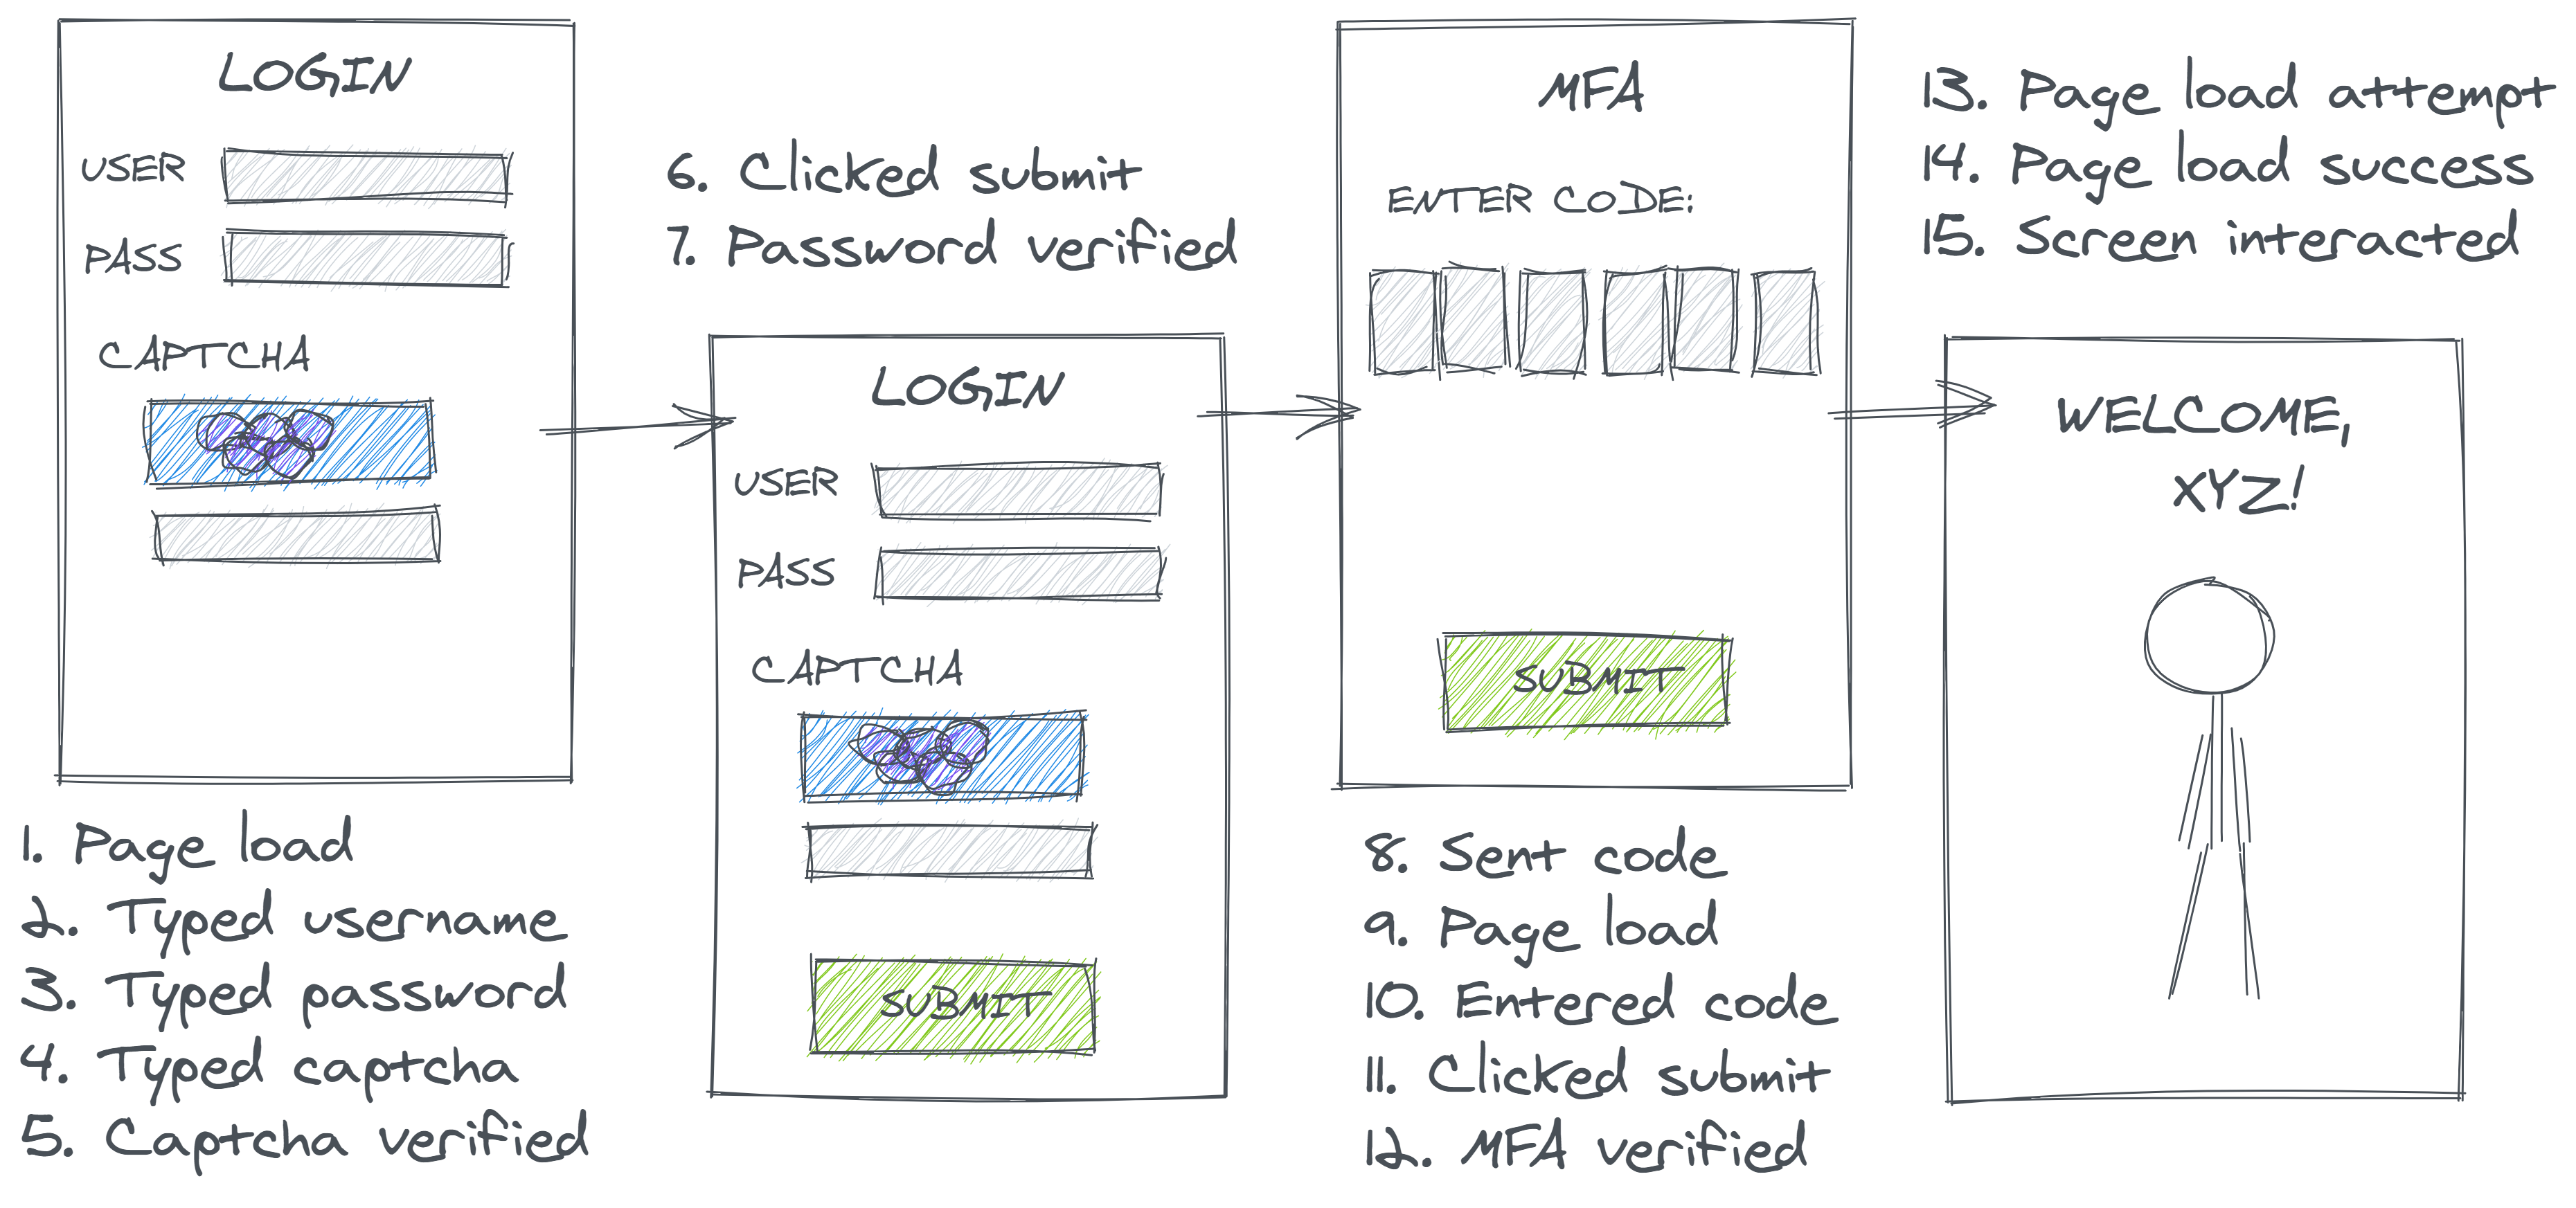
\includegraphics[width=0.9\linewidth]{figures/data-dall/login-log} 

}

\caption{A diagram illustrating a multi-step process for a user to login to a website or app}\label{fig:login-log}
\end{figure}

Which of these events gets collected and recorded has a significant impact on subsequent data processing.
In a technical sense, no inclusion/exclusion decision here is \emph{incorrect}, per say, but if the producers' choices don't match the consumers' understandings, it can lead to misleading results.

For example, an analyst might seek out a \texttt{logins} table in order to calculate the rate of successful website logins.
Reasonably enough, they might compute this rate as the sum of successful events over the total.
Now, suppose two users attempt to login to their account, and ultimately, one succeeds in accessing their private information and the other doesn't.
The analyst would probably hope to compute and report a 50\% login success rate. However, depending on how the data is represented, they could quite easily compute nearly any value from 0\% to 100\%.

As a thought experiment, we can consider what types of events might be logged:

\begin{itemize}
\tightlist
\item
  \textbf{Per Attempt}: If data is logged once per overall login attempt, successful attempts only trigger one event, but a user who forgot their password may try (and fail) to login multiple times. In the case illustrated above, that deflates the successful login rate to \textbf{25\%}.
\item
  \textbf{Per Event}: If the logins table contains a row for every login-related event, each `success' will trigger a large number of positive events and each `failure' will trigger a negative event preceded by zero or more positive events. In the case illustrated below, this inflates our successful login rate to \textbf{86\%}.
\item
  \textbf{Per Conditional}: If the collector decided to only look at downstream events, perhaps to circumvent record duplication, they might decide to create a record only to denote the success or failure of the final step in the login process (MFA). However, login attempts that failed an upstream step would not generate any record for this stage because they've already fallen out of the funnel. In this case, the computed rate could reach \textbf{100\%}
\item
  \textbf{Per Intermediate}: Similarly, if the login was defined specifically as successful password verification, the computed rate could his \textbf{100\%} even if some users subsequently fail MFA
\end{itemize}

These different situations are further illustrated in Figure \ref{fig:login-rate}, and their calculations are shown in Table \ref{tab:login-rate-tbl}.

\begin{figure}

{\centering 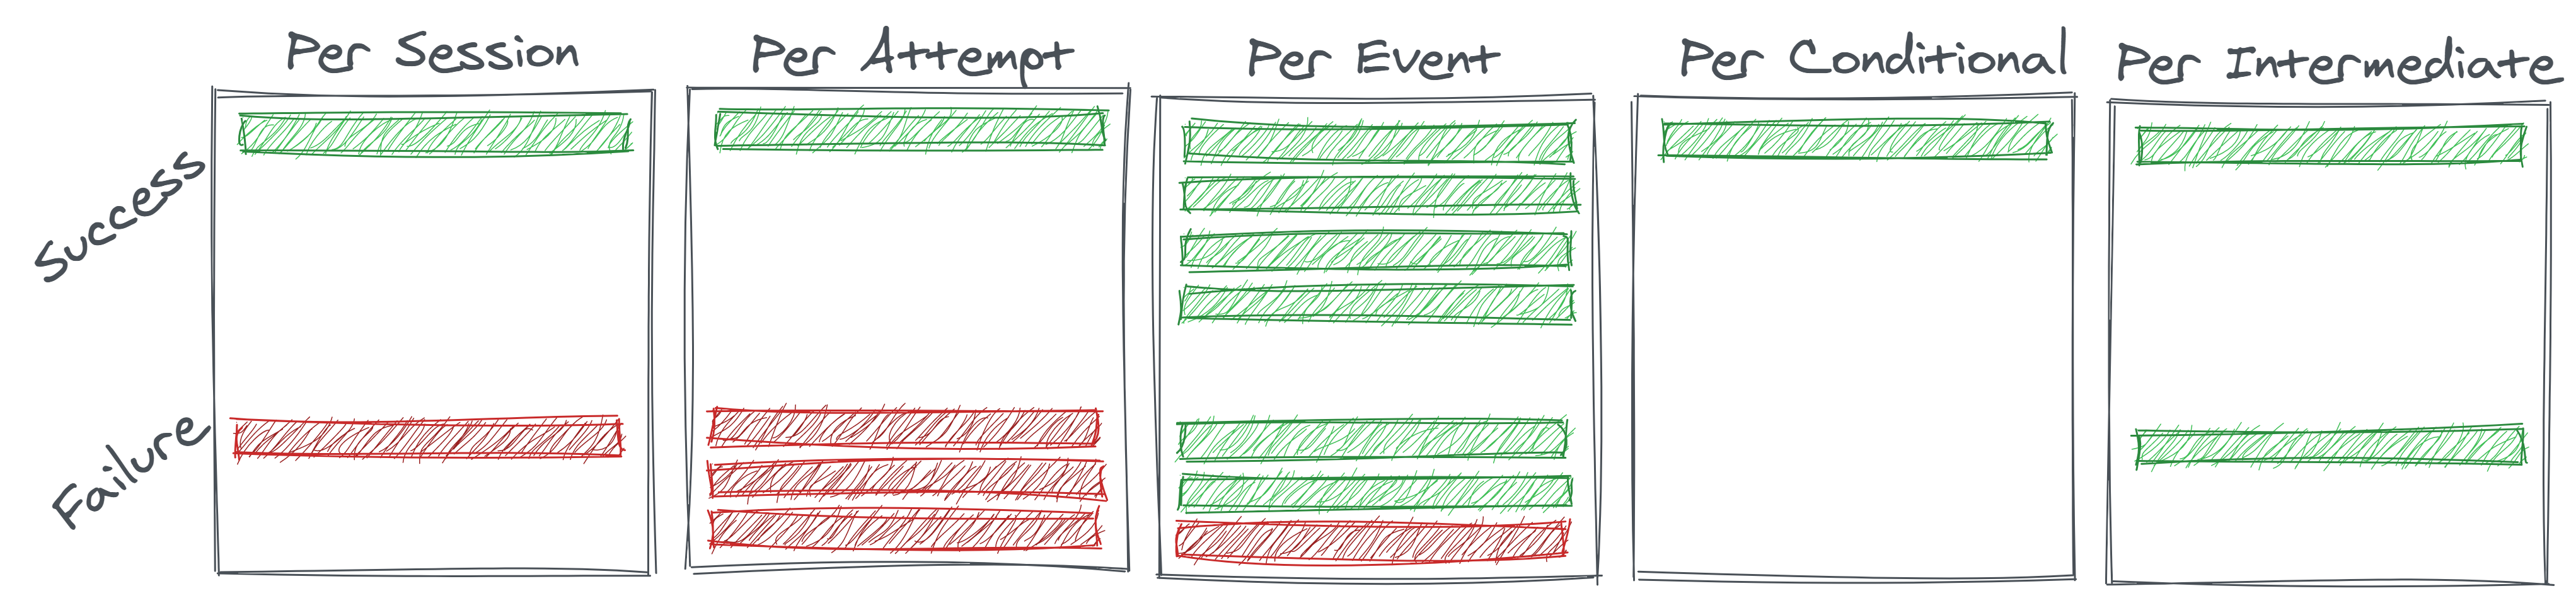
\includegraphics[width=0.9\linewidth]{figures/data-dall/login-rate} 

}

\caption{Login events recorded under different data collection paradigms}\label{fig:login-rate}
\end{figure}

\begin{table}

\caption{\label{tab:login-rate-tbl}Success rate naively computed under different data collection schemes}
\centering
\begin{tabular}[t]{l|r|r|r|r|r}
\hline
  & Session & Attempt & Event & Outcome & Intermediate\\
\hline
Success & 1 & 1 & 6 & 1 & 2\\
\hline
Total & 2 & 4 & 7 & 1 & 2\\
\hline
Rate (\%) & 50 & 25 & 86 & 100 & 100\\
\hline
\end{tabular}
\end{table}

(Note that we did not explicitly ``simulate'' data here, but the workflow is largely the same. We imagine a real-world process, how that might translate into a digital representation, and created a numerical example to understand the implications. Not all simulations require fancy code; sometimes paper and a pencil or a thought experiment works just fine.)

While humans have a shared intuition of what concepts like a user, session, or login are, the act of collecting data forces us to map that intuition onto an atomic event .
Any misunderstanding in precisely what that definition is can have massive impact on the perceived data quality; ``per event'' data will appear heavily duplicated if it is assumed to be ``per session'' data.

In some cases, this could be obvious to detect.
If the system outputs fields that are incredibly specific (e.g.~with some hyperbole, imagine a \texttt{step\_in\_the\_login\_process} field with values taking any of the human-readable descriptions of the fifteen processes listed in the image above), but depending how this source is organized (e.g.~in contrast to above, if we only have fields like \texttt{sourceid} and \texttt{processid} with unintuitive alphanumeric encoded values) and defined, it could be nearly impossible to understand the nuances without uncovering quality metadata or talking to a data producer.

\hypertarget{what-doesnt-make-a-record-row}{%
\subsection{What Doesn't Make a Record (Row)}\label{what-doesnt-make-a-record-row}}

Along with thinking about what \emph{does} count (or gets logged), it's equally important to understand what systemically does not generate a record. Consider users who have the intent or desire to login (motivated by a real-world DGP) but cannot find the login page, or users who load the login page but never click a button because they know that they've forgotten their password and see no way to request it.
Often, some of these corner cases may be some of the most critical and informative (e.g.~here, demonstrating some major flaws in our UI).
It's hard to \emph{computationally} validate what data doesn't exist, so \emph{conceptual} data validation is critical.

\hypertarget{records-versus-keys}{%
\subsection{Records versus Keys}\label{records-versus-keys}}

The preceding discussion on what types of real-world observations will or will not generate records in our resulting dataset is related to but distinct from another important concept from the world of relational databases: \textbf{primary keys}.

\textbf{Primary keys} are a minimal subset of variables in a dataset than define a unique record.
For example, in the previous discussion of customer logins this might consist of \textbf{natural keys}\footnote{Keys with semantic meanings that are naturally part of the dataset} such as the combination of a \texttt{session\_id} and a \texttt{timestamp} or \textbf{surrogate keys}\footnote{Keys without semantic meaning that exist primarily for the purpose of being keys} such as a global \texttt{event\_id} that is generated every time the system logs any event.

Understanding a table's primary keys can be useful for many reasons.
To name a few reasons, these fields are often useful for linking data from one table to another and for identifying data errors (if the uniqueness of these fields are not upheld).
They also can be suggestive of the true granularity of the table.

However, simply knowing a table's primary keys does \emph{not} resolve the issues we discussed in the prior two sections.
Any of the many different data collection strategies we considered are \emph{unique} by session and timestamp;
however, as we've seen, that is no guarantee that they \emph{must} contain every session and timestamp in the universe of events.

\hypertarget{what-defines-a-variable-column}{%
\subsection{What Defines a Variable (Column)}\label{what-defines-a-variable-column}}

Just as critical as understanding what constitutes a record (row) in a dataset is understanding the precise definition of each variable (column).
Superficially, this task seems easier: after all, each variable has a name which hopefully includes some semantic information. However, quite often this information can provide a false sense of security.
Just because you identify a variable with a promising sounding name, that does not mean that it is the most relevant data for your analysis.

For example, consider wanting to analyze patterns in customer spend amounts across orders on an e-commerce website.
You might find a table of orders with a field called \texttt{amt\_spend}. But what might this mean?

\begin{itemize}
\tightlist
\item
  If the dataset is sourced from a payment processor, it likely includes the total amount billed to a customers' credit card: including item prices less any discounts, shipping costs, taxes, etc. Alternatively, if this order was split across a gift card and a credit card, this field might only reflect the amount charged to the credit card
\item
  If the dataset is created for Finance, it might perhaps include only the total of item prices less discounts if this best corresponded to the data the Finance team needs for revenue reporting
\item
  Someone, somewhere, at some point might have assigned \texttt{amt\_spend} to the name of the variable containing gross spend (before accounting for any discounts) and there might be a different variable \texttt{amt\_spend\_net} which accounts for discounts applied
\end{itemize}

It's critical to understand what each variable \emph{actually} means.
The upside of this is that it forces analysts to more crisply think about their research questions and what the \emph{ideal} variables for their analysis would be.
As we've seen, concepts like ``spend'' may seem deceptively simple, but are not unambiguous.

\hypertarget{data-extraction-loading}{%
\section{Data Extraction \& Loading}\label{data-extraction-loading}}

Checking that data contains expected and \emph{only} expected records (that is, completeness, uniqueness, and timeliness) is one of the most common first steps in data validation.
However, the superficially simple act of loading data into a data warehouse or updating data between tables can introduce a variety of risks to data completeness which require different strategies to detect.
Data loading errors can result in data that is stale, missing, duplicate, inconsistently up-to-date across sources, or complete but for only a subset of the range you think.

While the data quality principles of \textbf{completeness}, \textbf{uniqueness}, and \textbf{timeliness} would suggest that records should exist once and only once, the reality of many haphazard data loading process means data may appear sometime between zero and a handful of times. Data loads can occur in many different ways.
For example, they might be:

\begin{itemize}
\tightlist
\item
  manually executed
\item
  scheduled (like a \href{https://en.wikipedia.org/wiki/Cron}{cron} job)
\item
  orchestrated (with a tool like \href{https://airflow.apache.org/}{Airflow} or \href{https://www.prefect.io/}{Prefect})
\end{itemize}

No approach is free from challenges.
For example, scheduled jobs risk executing before an upstream process has completed (resulting in stale or missing data);
poorly orchestrated jobs may be prevented from working due to one missing dependency or might allow multiple stream to get out of sync (resulting in multisource missing data).
Regardless of the method, all approaches must be carefully configured to handle failures gracefully to avoid creating duplicates, and the frequency at which they are executed may cause partial loading issues if it is incompatible with the granularity of the source data.

\hypertarget{data-load-failure-modes}{%
\subsubsection{Data Load Failure Modes}\label{data-load-failure-modes}}

To develop our understanding of the true data generating process and to formulate theories on how our data could be broken (and what we should validate), it is useful to understand the different ways data extraction and loading can fail.

Figure \ref{fig:data-load} illustrates a number of examples. Suppose that each row of boxes in the diagram represents one day of records in a table.

\begin{figure}

{\centering 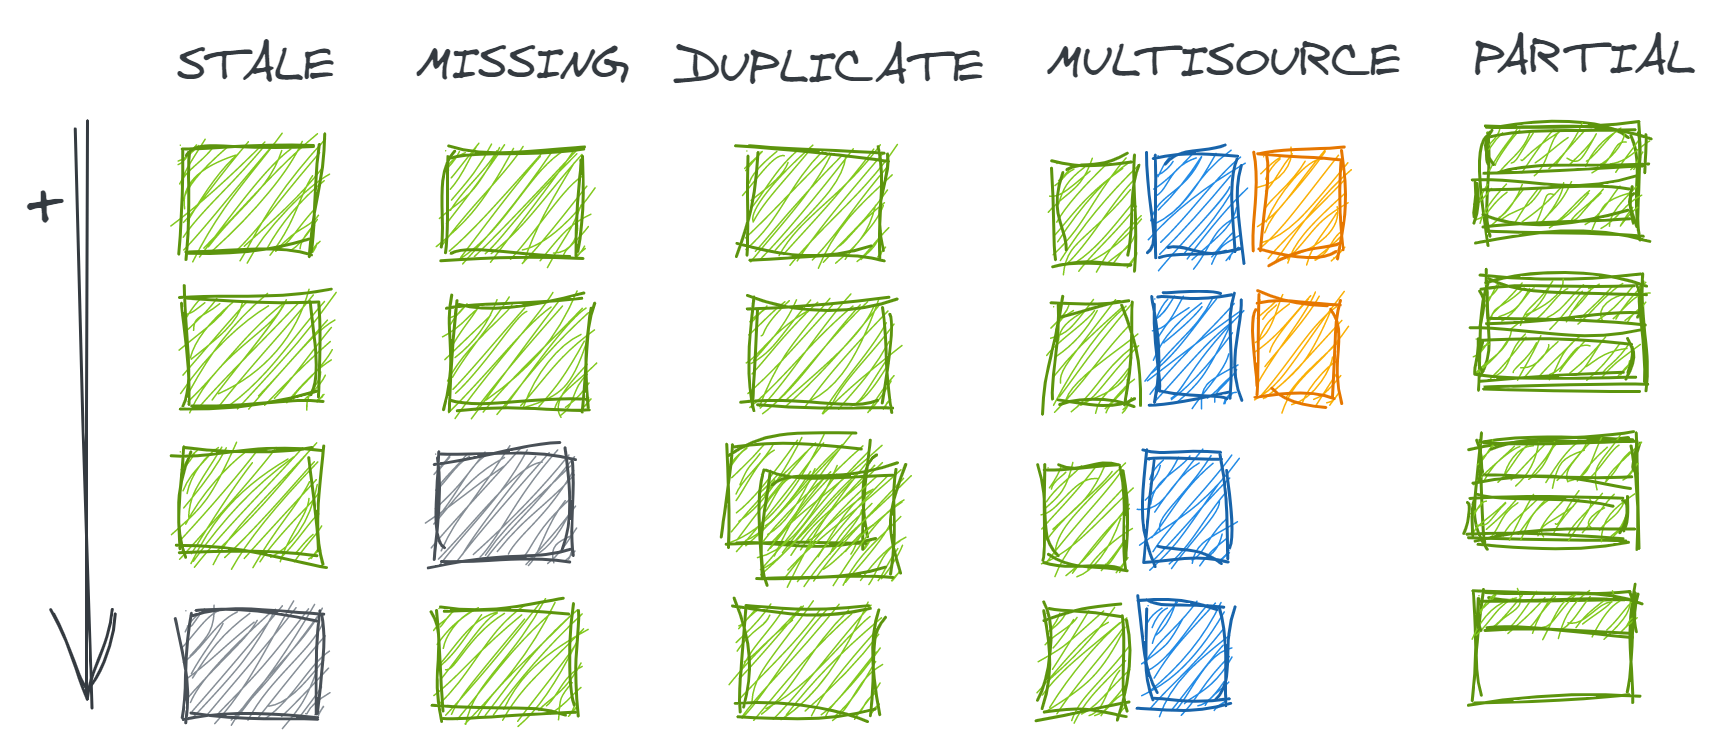
\includegraphics[width=0.9\linewidth]{figures/data-dall/data-load} 

}

\caption{Different modes of data loading failure}\label{fig:data-load}
\end{figure}

Our dataset might be susceptible to:

\begin{itemize}
\tightlist
\item
  \textbf{Stale data} occurs when the data is not as up-to-date as would be expected from is regular refresh cadence. This could happen if a manual step was skipped, a scheduled job was executed before the upstream source was available, or orchestrated data checks found errors and quarantined new records
\item
  \textbf{Missing data} occurs when one data load fails but subsequent loads have succeeded
\item
  \textbf{Duplicate data} occurs when one data load is executed multiple times
\item
  \textbf{Multisource missing data} occurs when a table is loaded from multiple sources, and some have continued to update as expected while others have not
\item
  \textbf{Partial data} occurs when a table is loaded correctly as intended by the producer but contains less data than expected by the consumer (e.g.~a table loads ever 12 hours but because there is some data for a given date, the user assumes that all relevant records for that date have been loaded)
\end{itemize}

The differences in these failure modes become important when an analyst attempts to assess data completeness.
One of the first approaches an analyst might consider is simply to check the \texttt{min()} and \texttt{max()} event dates in their table.
However, this can only help detect stale data.
To catch missing data, an analyst might instead attempt to count the number of \texttt{distinct} days represented in the data; to detect duplicate data, that analyst might need to count records by day and examine the pattern.

\begin{longtable}[]{@{}llllll@{}}
\toprule
\begin{minipage}[b]{0.14\columnwidth}\raggedright
Metric\strut
\end{minipage} & \begin{minipage}[b]{0.14\columnwidth}\raggedright
Stale\strut
\end{minipage} & \begin{minipage}[b]{0.14\columnwidth}\raggedright
Missing\strut
\end{minipage} & \begin{minipage}[b]{0.14\columnwidth}\raggedright
Duplicate\strut
\end{minipage} & \begin{minipage}[b]{0.14\columnwidth}\raggedright
Multi\strut
\end{minipage} & \begin{minipage}[b]{0.14\columnwidth}\raggedright
Partial\strut
\end{minipage}\tabularnewline
\midrule
\endhead
\begin{minipage}[t]{0.14\columnwidth}\raggedright
\texttt{min(date)} \texttt{max(date)}\strut
\end{minipage} & \begin{minipage}[t]{0.14\columnwidth}\raggedright
\textbf{13}\strut
\end{minipage} & \begin{minipage}[t]{0.14\columnwidth}\raggedright
14\strut
\end{minipage} & \begin{minipage}[t]{0.14\columnwidth}\raggedright
14\strut
\end{minipage} & \begin{minipage}[t]{0.14\columnwidth}\raggedright
14\strut
\end{minipage} & \begin{minipage}[t]{0.14\columnwidth}\raggedright
14\strut
\end{minipage}\tabularnewline
\begin{minipage}[t]{0.14\columnwidth}\raggedright
\texttt{count(distinct\ date)}\strut
\end{minipage} & \begin{minipage}[t]{0.14\columnwidth}\raggedright
\textbf{3}\strut
\end{minipage} & \begin{minipage}[t]{0.14\columnwidth}\raggedright
\textbf{3}\strut
\end{minipage} & \begin{minipage}[t]{0.14\columnwidth}\raggedright
4\strut
\end{minipage} & \begin{minipage}[t]{0.14\columnwidth}\raggedright
4\strut
\end{minipage} & \begin{minipage}[t]{0.14\columnwidth}\raggedright
4\strut
\end{minipage}\tabularnewline
\begin{minipage}[t]{0.14\columnwidth}\raggedright
\texttt{count(1)\ by\ date}\strut
\end{minipage} & \begin{minipage}[t]{0.14\columnwidth}\raggedright
\textbf{1001001000}\strut
\end{minipage} & \begin{minipage}[t]{0.14\columnwidth}\raggedright
\textbf{1001000100}\strut
\end{minipage} & \begin{minipage}[t]{0.14\columnwidth}\raggedright
\textbf{100100200100}\strut
\end{minipage} & \begin{minipage}[t]{0.14\columnwidth}\raggedright
1001006666\strut
\end{minipage} & \begin{minipage}[t]{0.14\columnwidth}\raggedright
10010010050\strut
\end{minipage}\tabularnewline
\begin{minipage}[t]{0.14\columnwidth}\raggedright
\texttt{count(1)} \texttt{count(distinct\ PKs)}\strut
\end{minipage} & \begin{minipage}[t]{0.14\columnwidth}\raggedright
300300\strut
\end{minipage} & \begin{minipage}[t]{0.14\columnwidth}\raggedright
300300\strut
\end{minipage} & \begin{minipage}[t]{0.14\columnwidth}\raggedright
\textbf{400300}\strut
\end{minipage} & \begin{minipage}[t]{0.14\columnwidth}\raggedright
332332\strut
\end{minipage} & \begin{minipage}[t]{0.14\columnwidth}\raggedright
350350\strut
\end{minipage}\tabularnewline
\bottomrule
\end{longtable}

In a case like the toy example above where the correct number of rows per date is highly predictable and the number of dates is small, such eyeballing is feasible;
however when the expected number of records varies day-to-day or time series are long, this approach becomes subjective, error-prone, and intractable.
Additionally, it still might be hard to catch errors in mutli-source data or partial loads if the lower number of records was still within the bounds of reasonable deviation for a series.
These last two types deserve further exploration.

\hypertarget{multi-source}{%
\subsubsection{Multi-Source}\label{multi-source}}

A more effective strategy for assessing data completeness requires a better understanding of how data is being collected and loaded.
In the case of multi-source data, one single source stopping loading may not be a big enough change to disrupt aggregate counts but could still jeopardize meaningful analysis.
It would be more useful to conduct completeness checks by \emph{subgroup} to identify these discrepancies.

But not any subgroup will do;
the subgroup must correspond to the various data sources.
For example, suppose we run an e-commerce store and wish to look at sales from the past month by category.
Naturally, we might think to check the completeness of the data by category.
But what if sales data is sourced from three separate locations: our Shopify site (80\%), our Amazon Storefront (15\%), and phone sales (5\%).
Unless we explicitly check completeness by channel (a dimension we don't particularly care about for our analysis), it would be easy to miss if our data source for phone sales has stopped working or loads at a different frequency.

Another interesting aspect of multi-source data, is multiple sources can contribute either to different \emph{rows/records} or different \emph{columns/variables}.
Table-level frequency counts won't help us in the latter case since other sources might create the right total number of records but result in some specific fields in those records being missing or inaccurate.

\hypertarget{partial-loads}{%
\subsubsection{Partial Loads}\label{partial-loads}}

Partial loads really are not data errors at all, but are still important to detect since they can jeopardize an analysis.
A common scenario might occur if a job loads new data every 12 hours (say, data from the morning and afternoon of day n-1 loads on day n at 12AM and 12PM, respectively).
An analyst retrieving data at 11AM may be concerned to see an approximate \textasciitilde50\% drop in sales in the past day, despite confirming that their data looks to be ``complete'' since the maximum record date is, in fact, day n-1.
Of course, this concern could be somewhat easily allayed if they then checked a timestamp field, but such a field might not exists or might not have been used for validation since its harder to anticipate the appropriate maximum timestamp than it is the maximum date.

\hypertarget{delayed-or-transient-records}{%
\subsubsection{Delayed or Transient Records}\label{delayed-or-transient-records}}

The interaction between choices made in the data collection and data loading phases can introduce their own sets of problems.

Consider an \texttt{orders} table for an e-commerce company that analysts may use to track customer orders.
It might contain one record per \texttt{order\_id} x \texttt{event} (placement, processing, shipment), one record per order placed, one record per order shipping, or one record per order with a \texttt{status} field that changes over time to denote the order's current stage of life. Some of these options are illustrated in Figure \ref{fig:order-log}.

\begin{figure}

{\centering 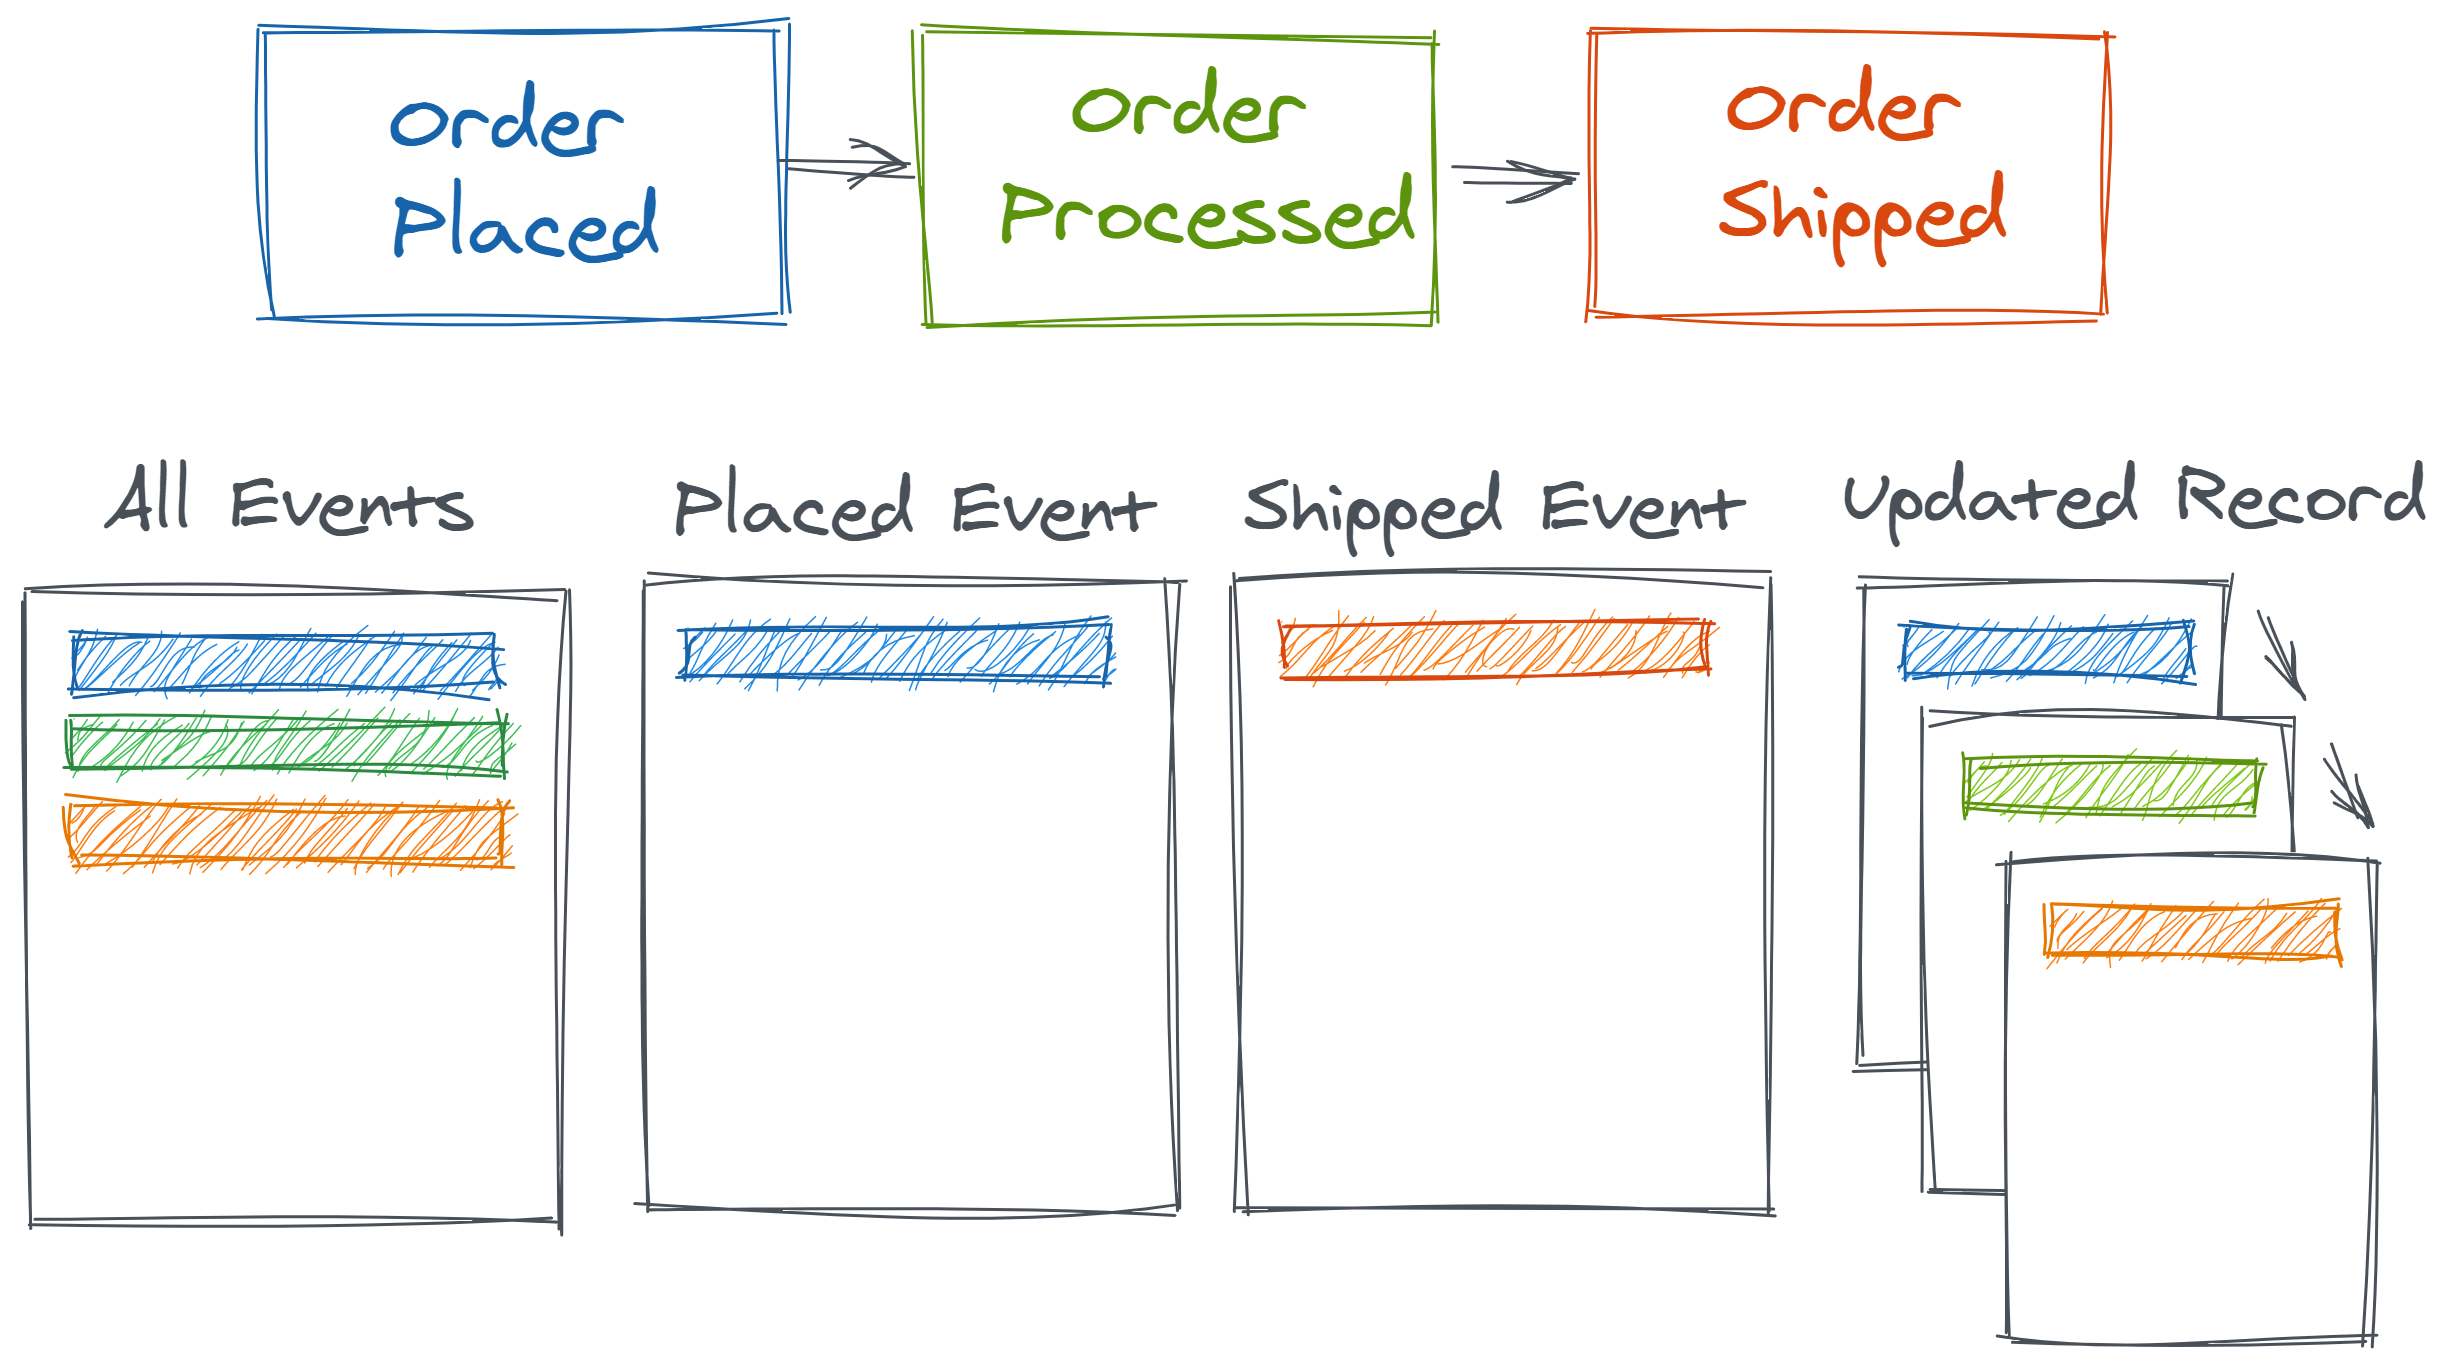
\includegraphics[width=0.9\linewidth]{figures/data-dall/order-log} 

}

\caption{Illustration of alternative data collection and extraction strategies for order data}\label{fig:order-log}
\end{figure}

Any of these modeling choices seem reasonable and the difference between them might appear immaterial.
But consider the \emph{collection} choice to record and report \emph{shipped} events.
Perhaps this might be operationally easier if shipment come from one source system whereas orders could come from many.
However, an interesting thing about shipments is that they are often lagged in a variable way from the order date.

Suppose the e-commerce company in question offers three shipping speeds at checkout. Figure \ref{fig:order-date} shows the range of possible shipment dates based on the order dates for the three different speeds (shown in different bars/colors).

\begin{figure}

{\centering 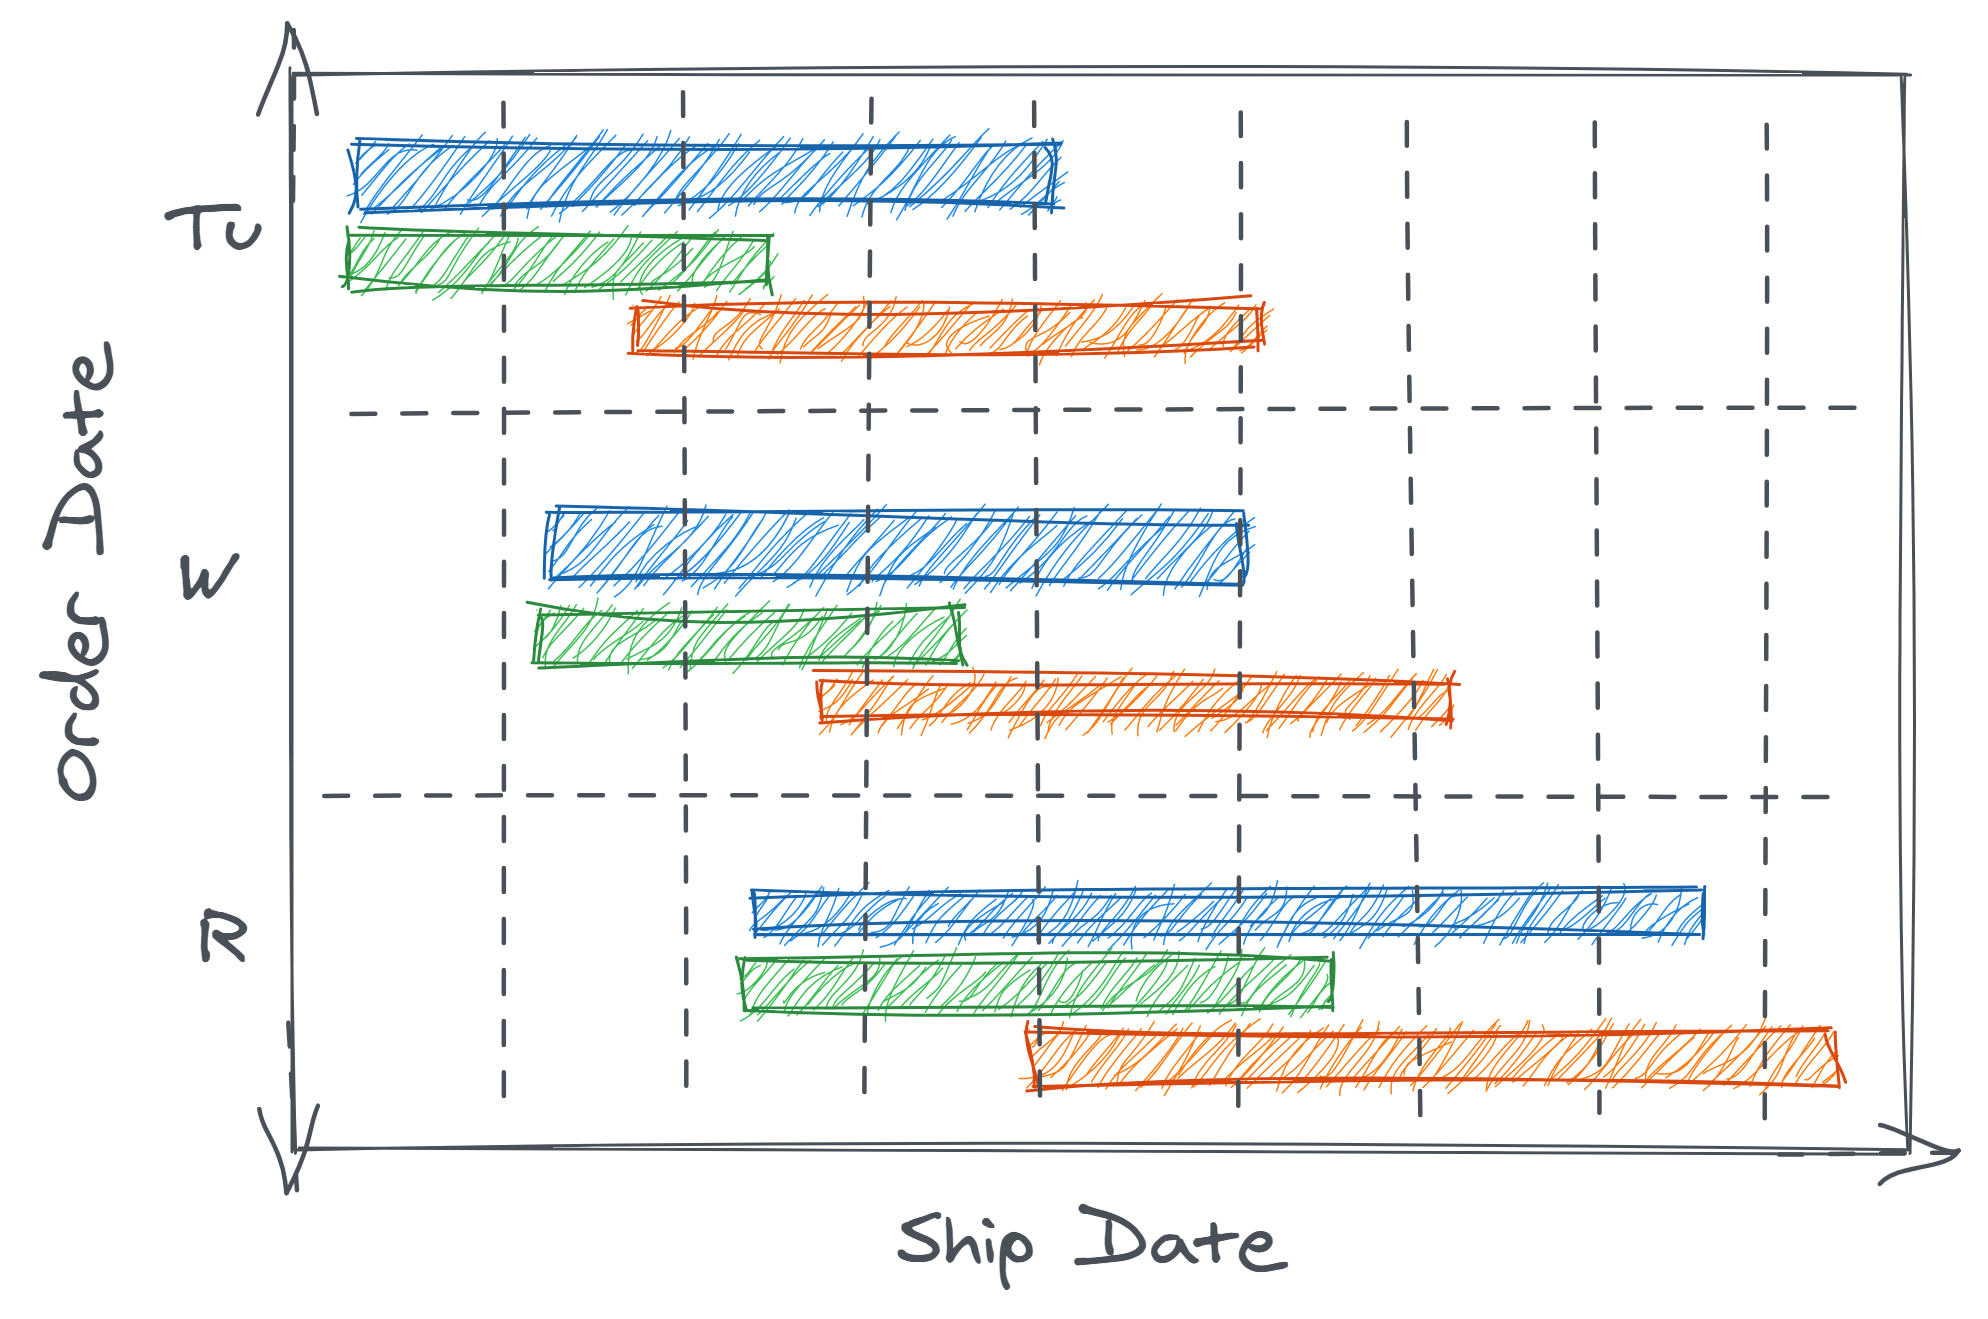
\includegraphics[width=0.9\linewidth]{figures/data-dall/order-date} 

}

\caption{A conceptual chart of when different classes of real-world events might materialize as records in our dataset}\label{fig:order-date}
\end{figure}

How might this effect our perceived data quality?

\begin{itemize}
\tightlist
\item
  Order data could appear \textbf{stale} or not timely since orders with a given \texttt{order\_date} would only load days later once shipped
\item
  Similar to \textbf{missing} or \textbf{multisource} data, the data \emph{range} in the table could lead to deceptive and incomplete data validation because some orders from a later order date might ship (and thus be logged) before all orders from a previous order date
\item
  Put another way, we could have multiple order dates demonstrating \textbf{partial} data loads
\item
  These features of the data might behave inconsistently across time due to seasonality (e.g.~no shipping on weekends or federal holidays), so heuristics developed to clean the data based on a small number of observations could fail
\item
  From an analytical perspective, orders with faster shipping would be disproportionately overrepresented in the ``tail'' (most recent) data. If shipping category correlated with other characteristics like total order spend, this could create an artificial trend in the data
\end{itemize}

Once again, understanding that data is \emph{collected} at point of shipment and reasoning how shipment timing varies and impacts \emph{loading} is necessary for successful validation.

If this thought experiment seems to vague, we can make it more concrete by mocking up a dataset with which to experiment.

In the simplest version, we will simply suppose one order is submited on each of 10 days with dates (represented for convenience as integers and not calendar dates) given by the \texttt{dt\_subm} vector.
Suppose shipping always takes three days, so we can easily calculate the shipment date (\texttt{dt\_ship}) based on the submission date.
The shipment date is the same as the date the data will be logged and loaded (\texttt{dt\_load}).

\begin{Shaded}
\begin{Highlighting}[]
\CommentTok{\# data simulation: single orders + deterministic ship dates {-}{-}{-}{-}}
\NormalTok{dt\_subm }\OtherTok{\textless{}{-}} \DecValTok{1}\SpecialCharTok{:}\DecValTok{10}
\NormalTok{days\_to\_ship }\OtherTok{\textless{}{-}} \DecValTok{3}
\NormalTok{dt\_ship }\OtherTok{\textless{}{-}}\NormalTok{ dt\_subm }\SpecialCharTok{+}\NormalTok{ days\_to\_ship}
\NormalTok{dt\_load }\OtherTok{\textless{}{-}}\NormalTok{ dt\_ship}
\NormalTok{df }\OtherTok{\textless{}{-}} \FunctionTok{data.frame}\NormalTok{(dt\_subm, dt\_ship, dt\_load)}
\FunctionTok{head}\NormalTok{(df)}
\end{Highlighting}
\end{Shaded}

\begin{verbatim}
##   dt_subm dt_ship dt_load
## 1       1       4       4
## 2       2       5       5
## 3       3       6       6
## 4       4       7       7
## 5       5       8       8
## 6       6       9       9
\end{verbatim}

Suppose we are an analyst living in day 5 and wonder how many orders were submitted on day 3.
We can observe all shipments loaded before day 5 so we filter our data accordingly.
However, when we count how many records exist for day 3 we find none.
Instead, when we move ahead to an analysis date of day 7, we are able to observe the orders submitted on day 3.

\begin{Shaded}
\begin{Highlighting}[]
\FunctionTok{library}\NormalTok{(dplyr)}

\CommentTok{\# how many day{-}3 orders do we observe as of day{-}5? {-}{-}{-}{-}}
\NormalTok{df }\SpecialCharTok{\%\textgreater{}\%} 
  \FunctionTok{filter}\NormalTok{(dt\_load }\SpecialCharTok{\textless{}=} \DecValTok{5}\NormalTok{) }\SpecialCharTok{\%\textgreater{}\%} 
  \FunctionTok{filter}\NormalTok{(dt\_subm }\SpecialCharTok{==} \DecValTok{3}\NormalTok{) }\SpecialCharTok{\%\textgreater{}\%} 
  \FunctionTok{nrow}\NormalTok{()}
\end{Highlighting}
\end{Shaded}

\begin{verbatim}
## [1] 0
\end{verbatim}

\begin{Shaded}
\begin{Highlighting}[]
\CommentTok{\# how many day{-}3 orders do we observe as of day{-}7? {-}{-}{-}{-}}
\NormalTok{df }\SpecialCharTok{\%\textgreater{}\%} 
  \FunctionTok{filter}\NormalTok{(dt\_load }\SpecialCharTok{\textless{}=} \DecValTok{7}\NormalTok{) }\SpecialCharTok{\%\textgreater{}\%} 
  \FunctionTok{filter}\NormalTok{(dt\_subm }\SpecialCharTok{==} \DecValTok{3}\NormalTok{) }\SpecialCharTok{\%\textgreater{}\%} 
  \FunctionTok{nrow}\NormalTok{()}
\end{Highlighting}
\end{Shaded}

\begin{verbatim}
## [1] 1
\end{verbatim}

(Note that these conditions could be checked much more succinctly with a base R expression such as \texttt{sum(df\$dt\_load\ \textless{}\ 7\ \&\ df\$dt\_subm\ ==\ 3)}.
However, there is sometimes virtue in option for more readable code even if it is less compact.
Here, we prefer the more verbose option for the claritfy of our exposition.
Such trade-offs, and general thoughts on coding style, are explored further in Chapter \ref{comp-code}.)

Now, this may seem to trivial. Clearly, if there were \emph{zero} records for a day, we would catch this in data validation, right?
We can make our synthetic data slightly more realistic to better illustrate the problem.
Let's not imagine that there are 10 orders each day, and each order is shipped sometime between 2 and 4 days after the order with equal probability.

\begin{Shaded}
\begin{Highlighting}[]
\CommentTok{\# data simulation: multiple orders + random ship dates {-}{-}{-}{-}}
\NormalTok{dt\_subm }\OtherTok{\textless{}{-}} \FunctionTok{rep}\NormalTok{(}\AttributeTok{x =} \DecValTok{1}\SpecialCharTok{:}\DecValTok{10}\NormalTok{, }\AttributeTok{each =} \DecValTok{10}\NormalTok{)}
\NormalTok{days\_to\_ship }\OtherTok{\textless{}{-}} \FunctionTok{sample}\NormalTok{(}\AttributeTok{x =} \DecValTok{2}\SpecialCharTok{:}\DecValTok{4}\NormalTok{, }\AttributeTok{size =} \FunctionTok{length}\NormalTok{(dt\_subm), }\AttributeTok{replace =} \ConstantTok{TRUE}\NormalTok{)}
\NormalTok{dt\_ship }\OtherTok{\textless{}{-}}\NormalTok{ dt\_subm }\SpecialCharTok{+}\NormalTok{ days\_to\_ship}
\NormalTok{dt\_load }\OtherTok{\textless{}{-}}\NormalTok{ dt\_ship}
\NormalTok{df }\OtherTok{\textless{}{-}} \FunctionTok{data.frame}\NormalTok{(dt\_subm, dt\_ship, dt\_load)}
\FunctionTok{head}\NormalTok{(df)}
\end{Highlighting}
\end{Shaded}

\begin{verbatim}
##   dt_subm dt_ship dt_load
## 1       1       4       4
## 2       1       5       5
## 3       1       5       5
## 4       1       5       5
## 5       1       4       4
## 6       1       4       4
\end{verbatim}

When we repeat the prior analysis, we now see that we have \emph{some} records for orders submitted on day 3 by the time we begin analysis on day 5.
In this case, we might be more easily tricked to believe this is \emph{all} orders.
However, when we repeat the analysis on day 7, we see the the number of orders on day 3 has increased.

Of course, you can imagine the real world is yet much more complicated than this example.
In reality, we would have a random number of orders each day.
Additionally, we might have a \emph{mixture} of different \emph{types} of orders.
There might be high-priced orders where customers tended to be willing to pay for faster shipping,
and low-priced orders where customers tend to chose slower shipping.
In a case like this, not only might naive validation miss the lack of data completeness, but the \emph{sample} of shipments we begin to see on day 5 could be unrepresentative of the population of orders placed on day 3.
This is a type of \textbf{selection bias} that we will examine further in Chapter \ref{incr-infe} (Incredible Inferences).

\hypertarget{data-encoding-transformation-wip}{%
\section{Data Encoding \& Transformation (WIP)}\label{data-encoding-transformation-wip}}

Once data is loaded into a more suitable location for processing and analysis (such as a data warehouse), it often undergoes numerous transformations to change its shape, structure, and content to be more suited for analytical use.

For example, recall the \texttt{logins} table that we discussed above. It might be filtered to a cleaner versions which represents only a subset of events, or event identifiers like \texttt{\textquotesingle{}1436\textquotesingle{}} might be recoded to more human-readable names like \texttt{\textquotesingle{}mfa-success\textquotesingle{}}.

Unfortunately, although these steps attempt to increase the data's usability, they are also not immune to inserting bugs.

\hypertarget{data-encoding}{%
\subsection{Data Encoding}\label{data-encoding}}

\hypertarget{data-types}{%
\subsubsection{Data Types}\label{data-types}}

One critical set of decisions in data encoding is what sort of \emph{data types} each field of interest should be. Data types such as integers, reals, character strings, logicals, dates, and times determine how data is stored and the types of manipulations that can be done to it.

We'll see more examples of the computational implications for our data types in Chapter \ref{comp-quan} (Computational Quandaries). This chapter specifically explores the unique complexities of string and date types.

\hypertarget{indicator-variables-todo}{%
\subsubsection{Indicator Variables (TODO)}\label{indicator-variables-todo}}

what is positive case?

\begin{quote}
``We had a bunch of zeros that should have been coded ones and the ones should have been coded zeroes.''
\end{quote}

(\url{https://retractionwatch.com/2013/01/04/paper-on-evidence-for-environmental-racism-in-epa-polluter-fines-retracted-for-coding-error/})

\hypertarget{general-representation-todo}{%
\subsubsection{General Representation (TODO)}\label{general-representation-todo}}

\begin{quote}
``These data sets often have multiple files that\ldots have unclear and sometimes duplicative variables. Such complexities are commonplace among many data systems\ldots{} I would not be surprised if coding errors were fairly common, and that the ones discovered constitute only the ``tip of the iceberg.''
''
\end{quote}

(\url{https://retractionwatch.com/2015/09/10/divorce-study-felled-by-a-coding-error-gets-a-second-chance/})

\hypertarget{the-many-meanings-of-null}{%
\subsubsection{The Many Meanings of Null}\label{the-many-meanings-of-null}}

Another major encoding decision is how to handle null values.
Previously, in the discussion of Data Collection, we considered the presence and absence of full \emph{records}.
However, when preparing data for analysis, both data produces and consumers need to decide how to cope with the presence or absence of individual \emph{fields}.

If records contain some but not all relevant information, they may be published with explicitly missing fields or the full record may not be published at all. The difference between implicit and explicit missingness on the resulting data is illustrated in Figure \ref{fig:null-impl-expl}.

\begin{figure}

{\centering 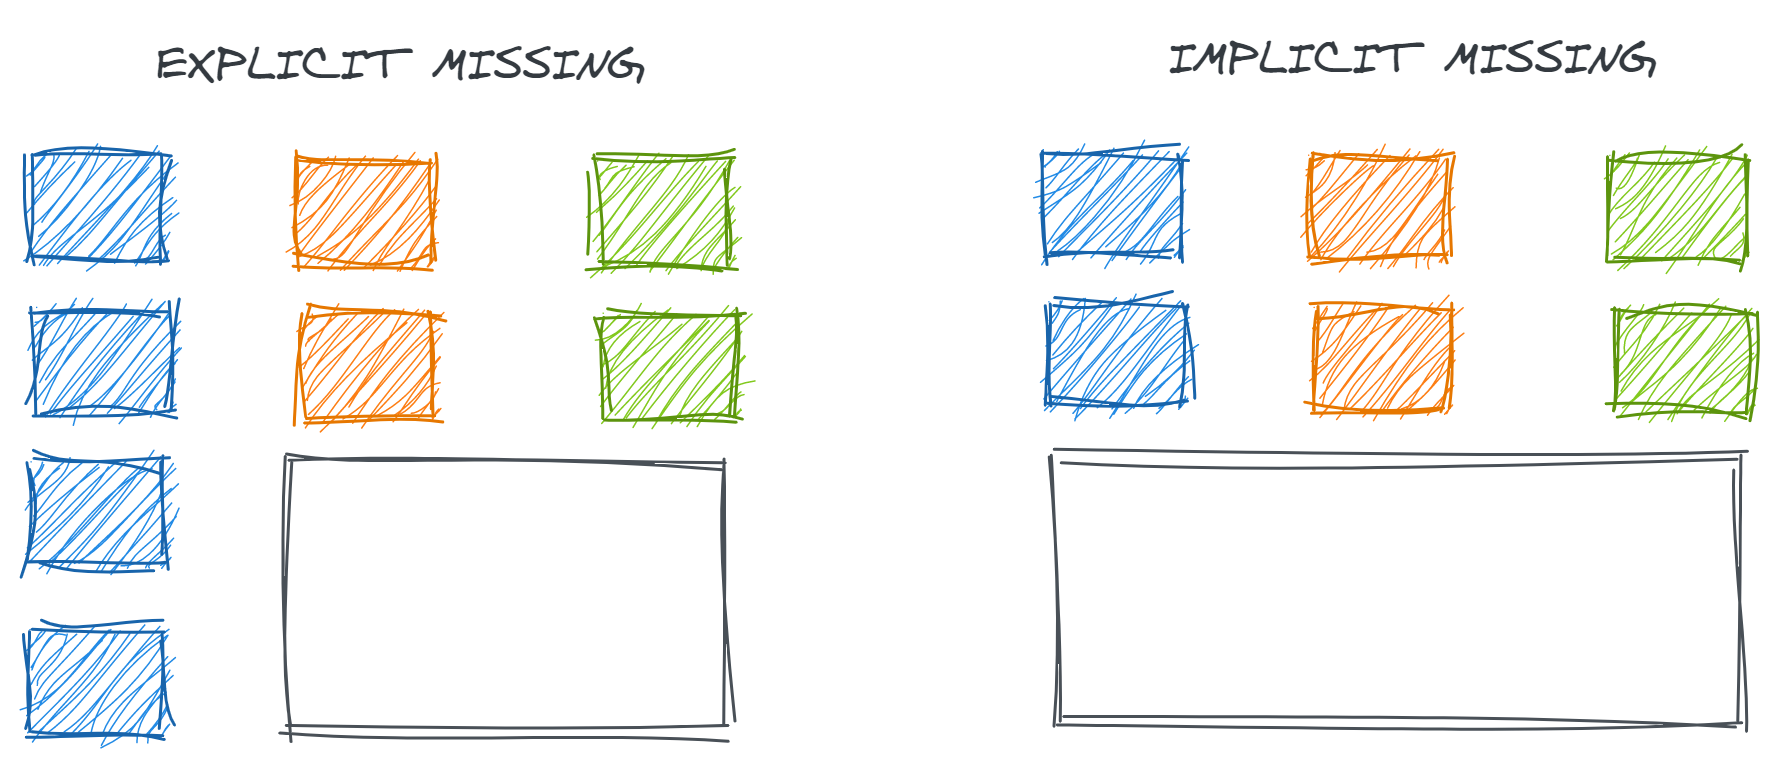
\includegraphics[width=0.9\linewidth]{figures/data-dall/missing-imp-exp} 

}

\caption{A comparison of explicit versus implicit missingness}\label{fig:null-impl-expl}
\end{figure}

Understanding what the system implies by each \emph{explicitly} missing data field is also critical for validation and analysis.
Checks for data completeness usually include counting null values, but null data isn't always incorrect.
In fact, null data can be highly informative if we know what it means. Some meanings of null data might include:

\begin{itemize}
\tightlist
\item
  \textbf{Field is not relevant}: Perhaps our \texttt{logins} table reports the mobile phone operating system (iOS or Android) that was used to access the login page to track platform-specific issues. However, there is no valid value for this
\item
  \textbf{Relevant value is not known}: Our \texttt{logins} table might also have an \texttt{account\_id} field which attempts to match login attempts to known accounts/customers using different metadata like cookies or IP addresses. In theory, almost everyone trying to log in should have an account identifier, but our methods may not be good enough to identify them in all cases
\item
  \textbf{Relevant value is null}: Of course, sometimes someone without an account at all might try to log in for some reason. In this case, the correct value for an \texttt{account\_id} field truly \emph{is} null
\item
  \textbf{Relevant value was recorded incorrectly}: Sometimes systems have glitches. Without a doubt, every single login attempt \emph{should} have a timestamp, but such a field could be null if this data was somehow lost or corrupted at the source
\end{itemize}

Similarly, different systems might or might not report out these nulls in different ways such as:

\begin{itemize}
\tightlist
\item
  \textbf{True nulls}: Literally the entry in the resulting dataset is null
\item
  \textbf{Null-like non-nulls}: Blank values like an empty string (\texttt{\textquotesingle{}\textquotesingle{}}) that contain a null amount of information but won't be detected when counting null values
\item
  \textbf{Placeholder values}: Meaningless values like an \texttt{account\_id} of \texttt{00000000} for all unidentified accounts which preserve data \emph{validity} (the expected structure) but have no intrinsic meaning
\item
  \textbf{Sentinel/shadow values}: Abnormal values which attempt to indicate the reasons for null-ness such as an \texttt{account\_id} of \texttt{-1} when no browser cookies were found or \texttt{-2} when cookies were found but did not help link to any specific customer record
\end{itemize}

Each of these encoding choices changes the definitions of appropriate completeness and validity for each field and, even more critically, impacts the expectations and assertions we should form for data accuracy.
We can't expect 100\% completeness if nulls are a relevant value; we can't check validity of ranges as easily if sentinel values are used with values that are outside the normal range (hopefully, or we have much bigger problems!)
So, understanding how upstream systems \emph{should} work is essential for assessing if they \emph{do} work.

Similarly, understanding how our null data is collected has significant implications for how we subsequently process it. We will discuss this more in Chapter \ref{comp-quan} (Computational Quandaries).

\hypertarget{data-transformation}{%
\subsection{Data Transformation}\label{data-transformation}}

Finally, once the data is roughly where we want it, it likely undergoes many transformations to translate all of the system-generated fields we discussed in data collection into semantically-relevant dimensions for analytical consumers. Of course, the types of transformations that could be done are innumerable with far more variation than data loading. So, we'll just look at a few examples of common failure patterns.

\hypertarget{pre-aggregation}{%
\subsubsection{Pre-Aggregation}\label{pre-aggregation}}

Data transformations may include aggregating data up to higher levels of granularity for easier analysis. For example, a transformation might add up item-level purchase data to make it easier for an analyst to look at spend per \emph{order} of a specific user.

Data transformations not only transform our data, but they also transform how the dimensions of data quality manifest. If data with some of the \textbf{completeness} or \textbf{uniqueness} issues we discussed with data loading is pre-aggregated, these problems can turn into problems of \textbf{accuracy}. For example, the duplicate or partial data loads that we discussed when aggregated could suggest inaccurately high or low quantities respectively.

\begin{center}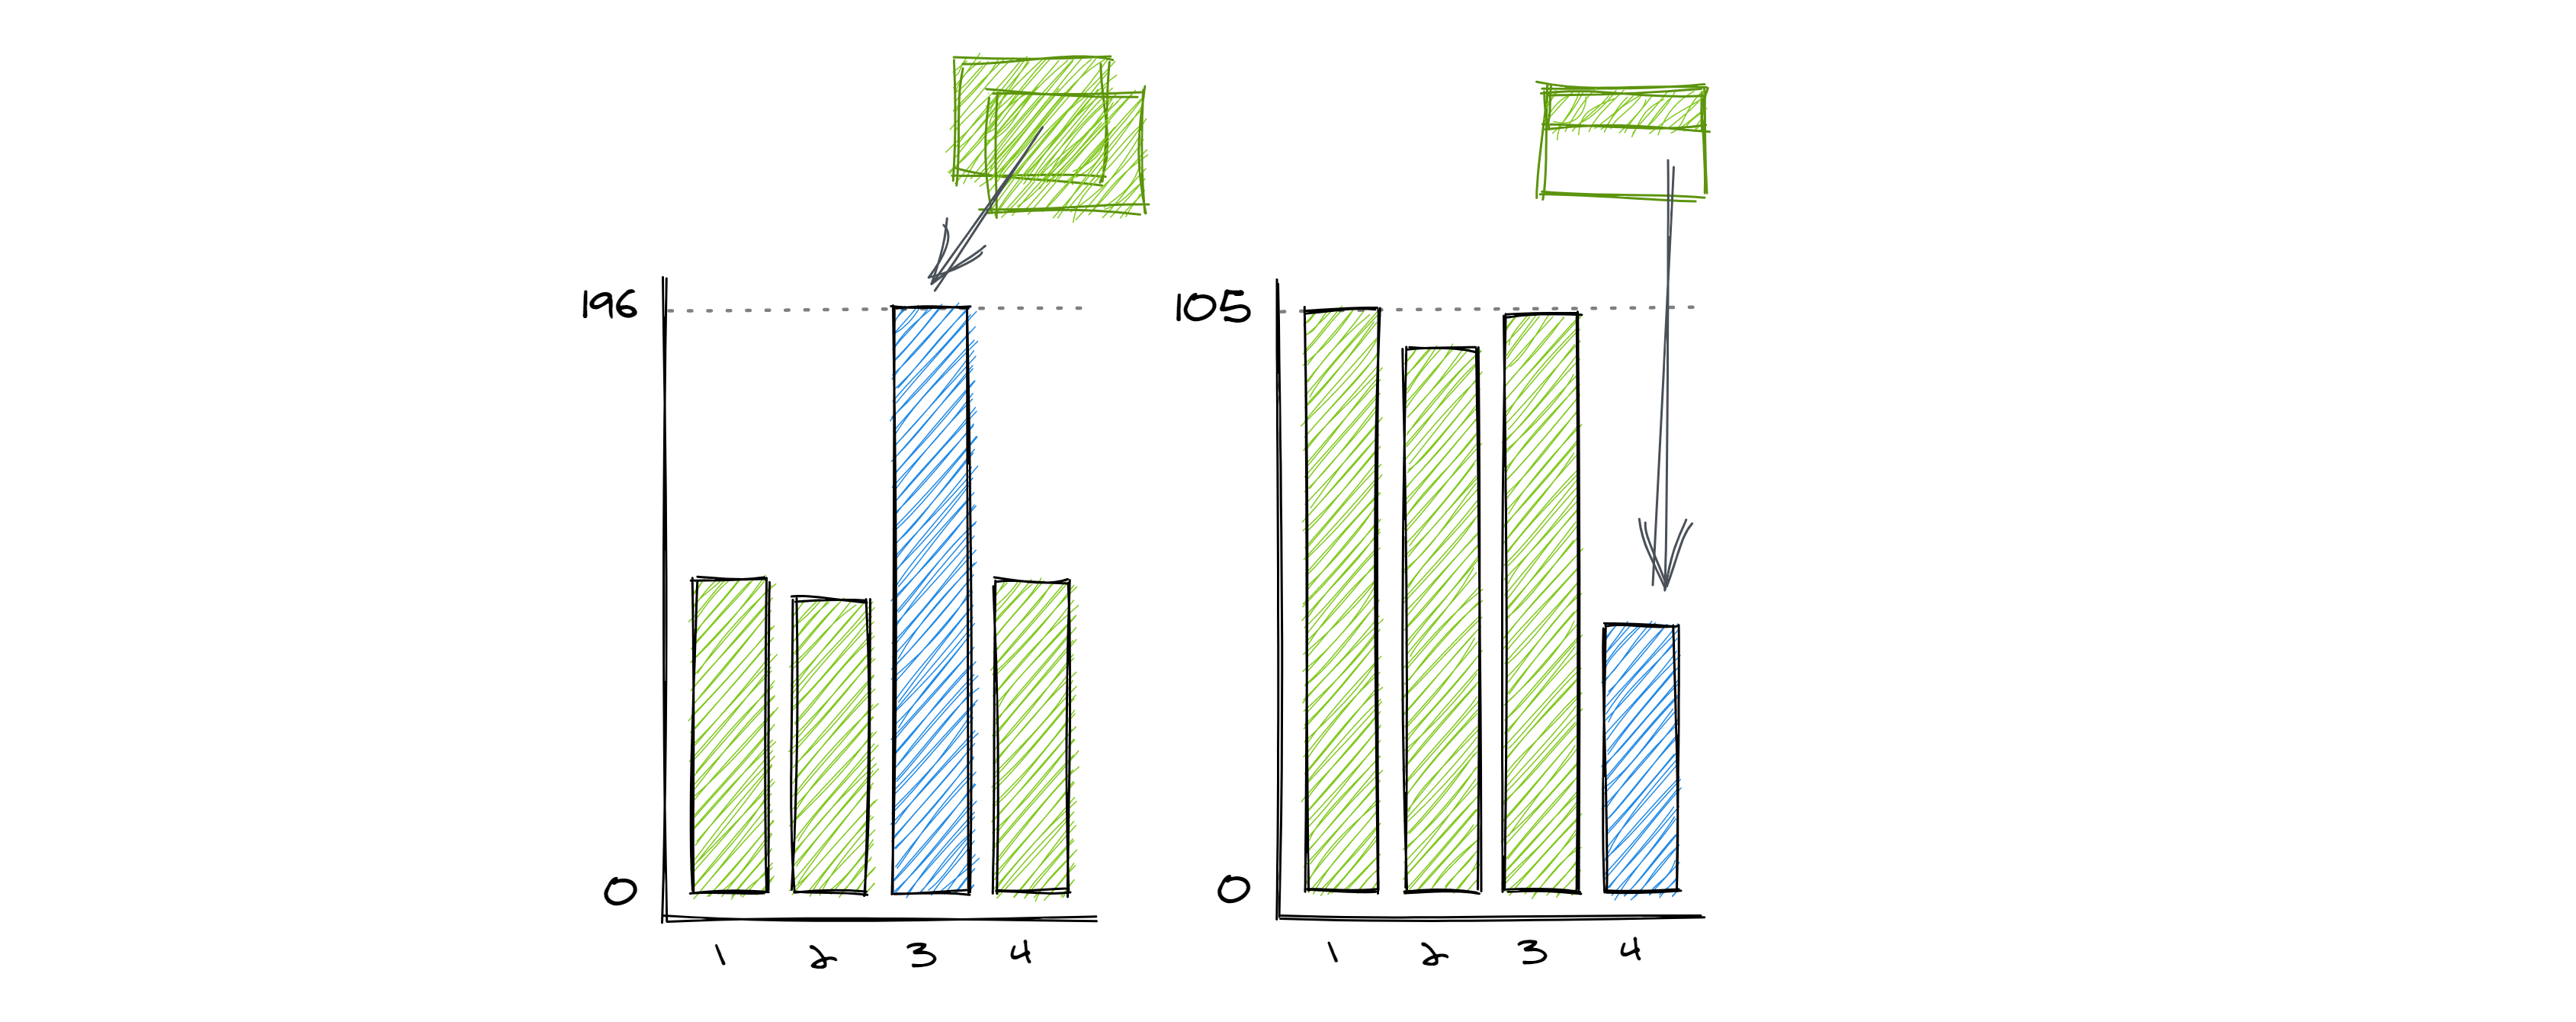
\includegraphics[width=0.9\linewidth]{figures/data-dall/completeness-accuracy} \end{center}

\hypertarget{field-encoding}{%
\subsubsection{Field Encoding}\label{field-encoding}}

When we assess data consistency across tables,

Categorical fields in a data set might be created in any number of ways including:

\begin{itemize}
\tightlist
\item
  Directly taken from the source
\item
  Coded in a transformation script
\item
  Transformed with logic in a shared user-defined function (\href{https://docs.snowflake.com/en/sql-reference/user-defined-functions.html}{UDFs}) or \href{https://docs.getdbt.com/docs/building-a-dbt-project/jinja-macros/\#macros}{macro}
\item
  Joined from a shared look-up table
\end{itemize}

Each approach has different implications on data consistency and usability.

\begin{center}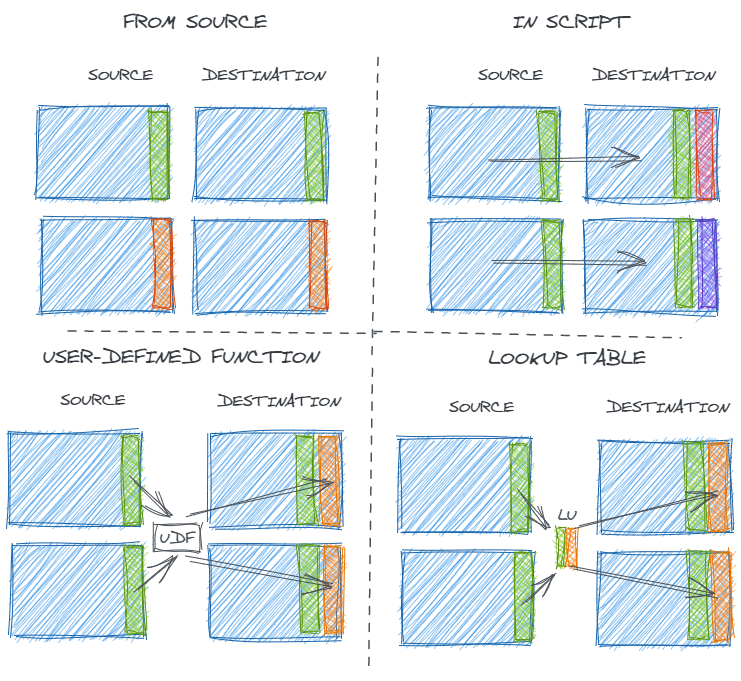
\includegraphics[width=0.9\linewidth]{figures/data-dall/field-encoding} \end{center}

Using fields from the source simply is what it is -- there's no subjectivity or room for manual human error. If multiple tables come from the same source, it's likely but not guaranteed that they will be encoded in the same way.

Coding transformations in the ELT process is easy for data producers. There's no need to coordinate across multiple processes or use cases, and the transformation can be immediately modified when needed. However, that same lack of coordination can lead to different results for fields that should be the same.

Alternatively, macros, UDFs, and look-up tables provided centralized ways to map source data inputs to desired analytical data outputs in a systemic and consistent way. Of course, centralization has its own challenges. If something in the source data changes, the process of updating a centralized UDF or look-up table may be slowed down by the need to seek consensus and collaborate. So, data is more \emph{consistent} but potentially less \emph{accurate}.

Regardless, such engineered values require scrutiny -- paticularly if they are being used as a key to join multiple tables -- and the distinct values in them should be carefully examined.

\hypertarget{updating-transformations}{%
\subsubsection{Updating Transformations}\label{updating-transformations}}

Of course, data consistency is not only a problem across different data sources but within one data source. Regardless of the method of field encoding used in the previous step, the intersection of data loading and data transformation strategies can introduce data consistency errors over time.

Often, for computation efficiency, analytical tables are loaded using an \emph{incremental} loading strategy. This means that only new records (determined by time period, a set of unique keys, or other criteria) from the upstream source are loaded to the downstream table. This is in contrast to a \emph{full refresh} where the entire downstream table is recreated on each update.

\begin{center}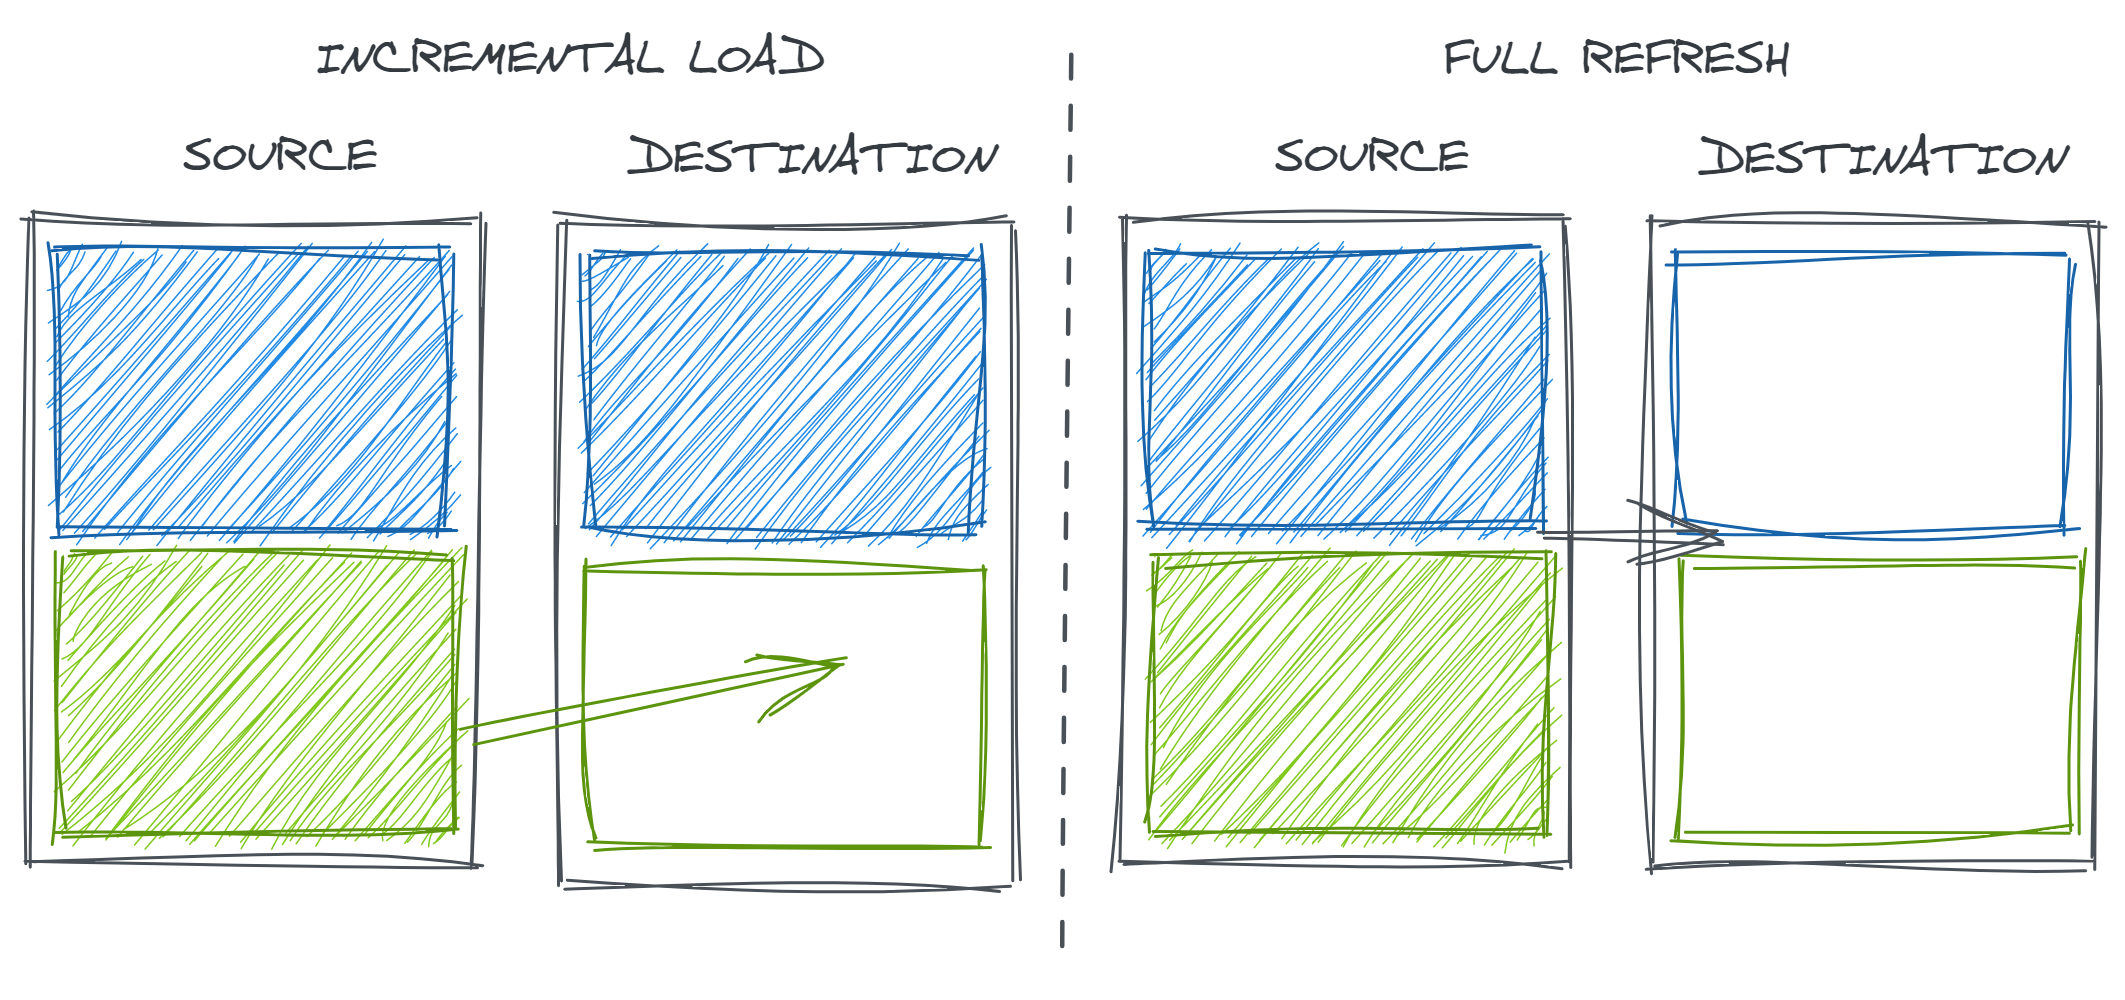
\includegraphics[width=0.9\linewidth]{figures/data-dall/incr-full-good} \end{center}

Incremental loads have many advantages. Rebuilding tables in entirety can be very time consuming and computationally expensive. In particular, in non-cloud data warehouses that are not able to scale computing power on demand, this sort of heavy duty processing job can noticeably drain resources from other queries that are trying to run in the database. Additionally, if the upstream staging data is ephemeral, fully rebuilding the table could mean failing to retain history.

However, in the case that our data transformations change, incremental loads may introduce inconsistency in our data overtime as only new records are created and inserted with the new logic.

\begin{center}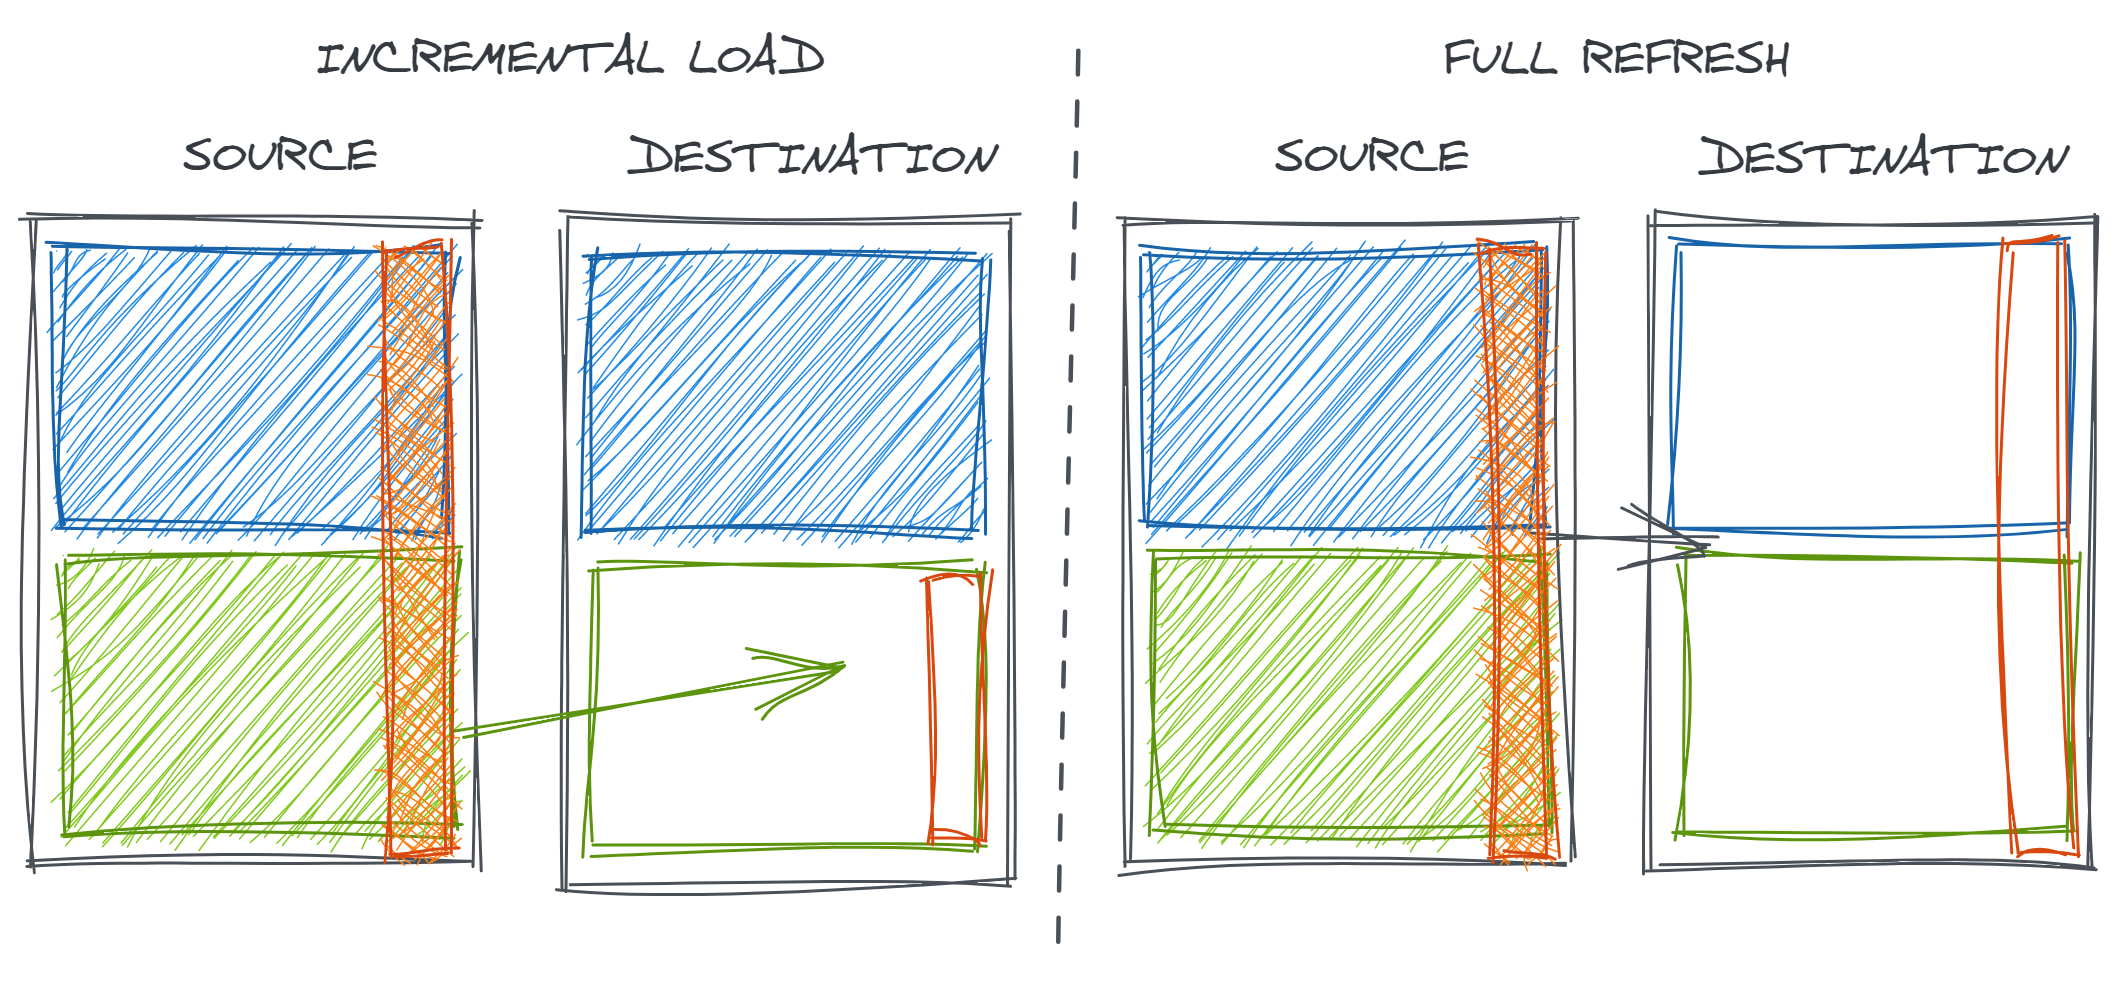
\includegraphics[width=0.9\linewidth]{figures/data-dall/incr-full-bad-col} \end{center}

This is also a problem more broadly if some short-term error is discovered either with data loading or transformation in historical data. Incremental strategies may not always update to include the corrected version of the data.

\begin{center}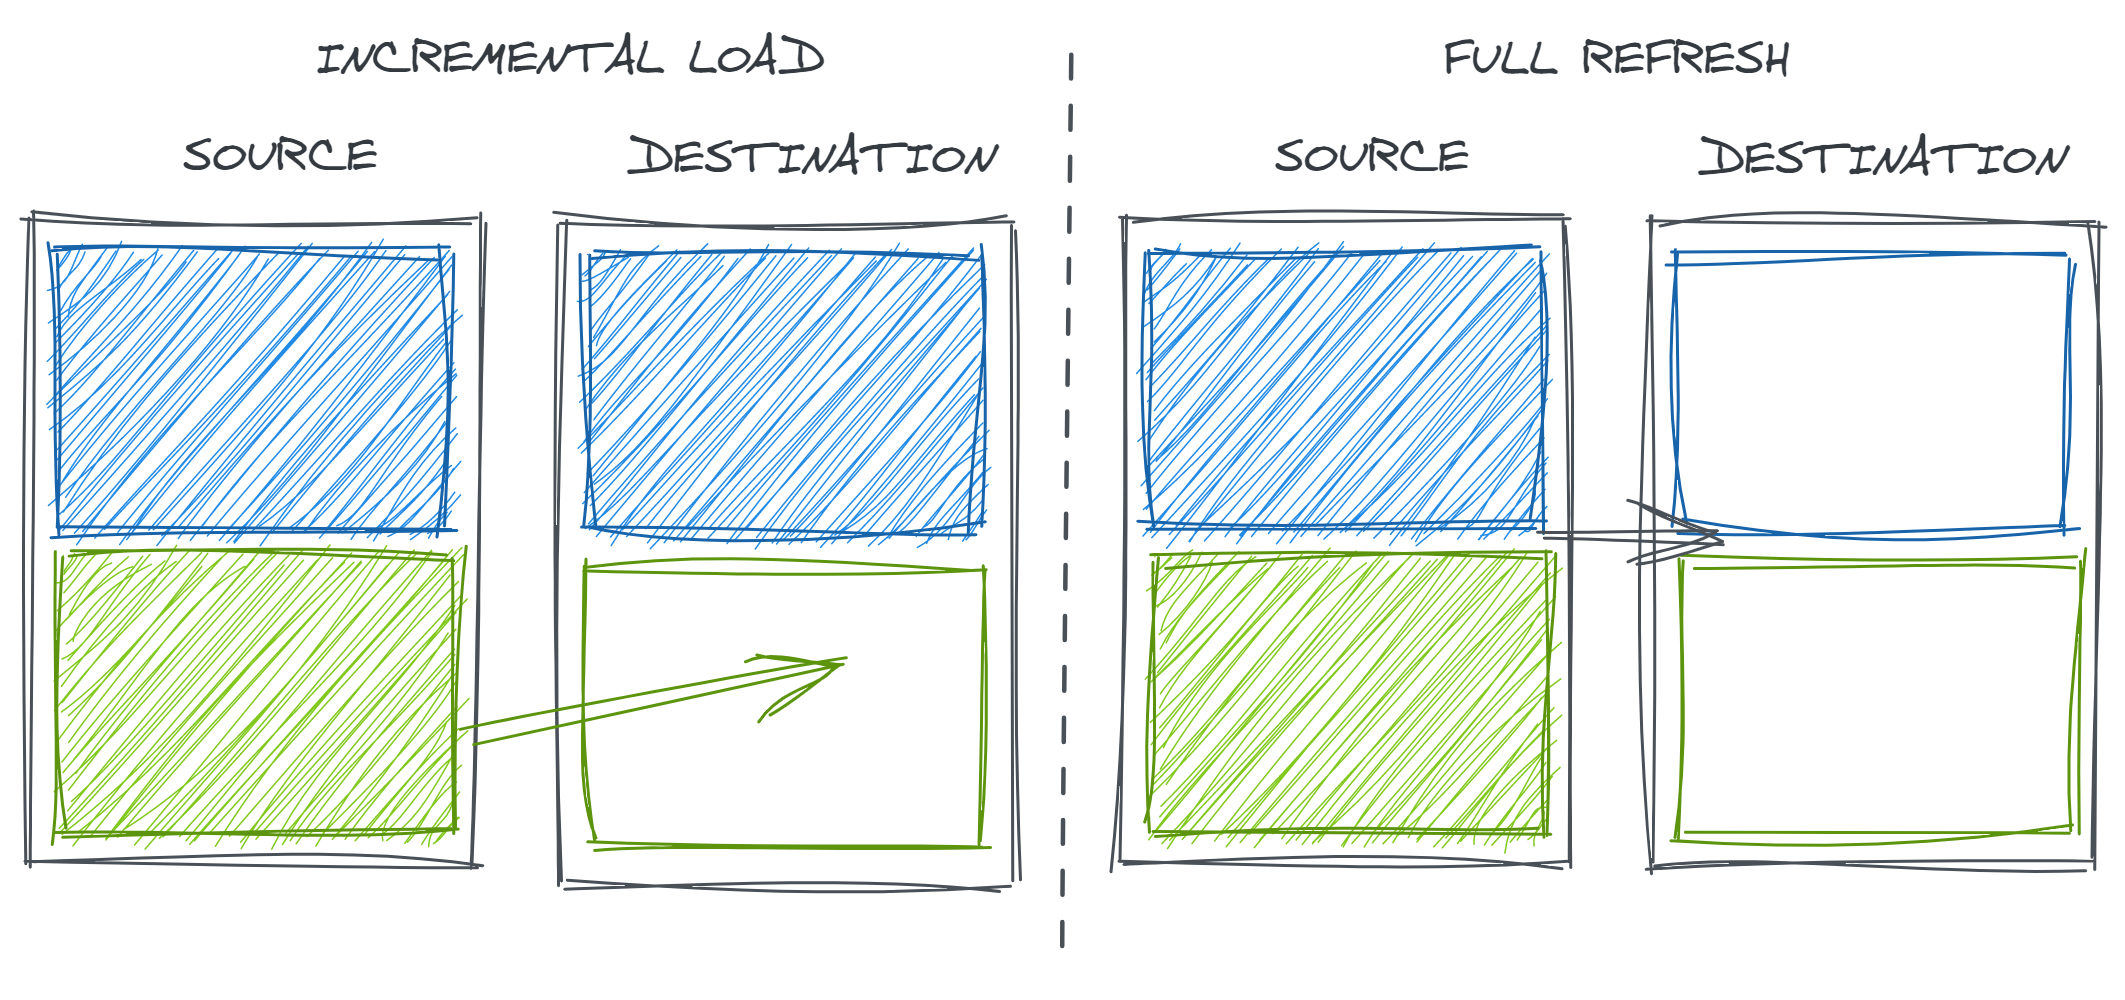
\includegraphics[width=0.9\linewidth]{figures/data-dall/incr-full-good} \end{center}

Regardless, this underscores the need to validate entire datasets and to re-validate when repulling data.

\hypertarget{other-types-of-data-todo}{%
\section{Other Types of Data (TODO)}\label{other-types-of-data-todo}}

\hypertarget{survey-data}{%
\subsection{Survey Data}\label{survey-data}}

\hypertarget{human-generated}{%
\subsection{Human-Generated}\label{human-generated}}

\hypertarget{strategies-todo}{%
\section{Strategies (TODO)}\label{strategies-todo}}

\hypertarget{understand-the-intent}{%
\subsection{Understand the intent}\label{understand-the-intent}}

\begin{itemize}
\tightlist
\item
  Why was data originally collected? By whom and for what purpose?
\item
  Are there clear, unique definitions of key concepts (e.g.~entites, measures)? What are they?
\item
  Documentation (metadata, dictionaries)
\end{itemize}

\hypertarget{understand-the-execution}{%
\subsection{Understand the execution}\label{understand-the-execution}}

\begin{itemize}
\tightlist
\item
  learn about the real-world systems
\item
  understand key steps in data production process
\item
  documentation (lineage, provenance)
\end{itemize}

\hypertarget{seek-expertise}{%
\subsection{Seek expertise}\label{seek-expertise}}

\begin{itemize}
\tightlist
\item
  talking to experts (upstream and downstream)
\end{itemize}

\hypertarget{trust-but-verify}{%
\subsection{Trust but verify}\label{trust-but-verify}}

\begin{itemize}
\tightlist
\item
  always on data validation

  \begin{itemize}
  \tightlist
  \item
    summaries
  \item
    context-informed assertions
  \end{itemize}
\item
  exploratory analysis
\end{itemize}

\hypertarget{real-world-disasters}{%
\section{Real World Disasters}\label{real-world-disasters}}

\hypertarget{data-loading-artificially-spikes-covid-cases}{%
\subsection{Data loading artificially spikes COVID cases}\label{data-loading-artificially-spikes-covid-cases}}

Data loading, particularly when a new process is introduced can go astray and lead to spurious results.
The city of El Paso discovered this after reporting an exceedingly high number of daily COVID cases \citep{borunda_2020}:

\begin{quote}
El Paso city and public health officials on Thursday admitted to a major blunder, saying that the more than 3,100 new cases reported a day earlier was incorrect.
\end{quote}

\begin{quote}
The number was the result of a two-day upload of cases in one day after the public health department went from imputing data manually to an automatic data upload that was intended to increase efficiency, Public Health Director Angela Mora said at news conference.
\end{quote}

This instance demonstrates not only how \emph{data} goes wrong but also how easy it is to trust discrepancies and find explanations in real-world phenomena.
The article goes on to suggest that the extremely high case numbers were not immediately caught given the overall ``alarming'' levels:

\begin{quote}
Mora said she accepted responsibility and that she should have taken a deeper look after noticing the abnormally high number of new cases.El Paso County is still seeing more than 1,000 new cases on a daily basis, officials said. The correct number of new cases Wednesday was 1,537.
\end{quote}

\begin{quote}
``The numbers are still high and they are still alarming but they were not as high as we reported,'' Mora said.
\end{quote}

\hypertarget{data-encoding-leads-to-incorrect-bmi-calculation}{%
\subsection{Data encoding leads to incorrect BMI calculation}\label{data-encoding-leads-to-incorrect-bmi-calculation}}

Data that is encoded inconsistently may be mishandled in automated decision processes.
For example, data manually entered into electronic health records (EHR) by countless care provides might be compiled into a single source although the meanings could be inconsistent.

In the early days of the COVID19 vaccination push, some regions chose to prioritize their vaccine supply by certain individual characteristics including a high body mass index (BMI), which is a function of one's weight relative to their height.

One 6ft 2in tall man's data was misinterpreted to suggest that he was 6.2 \emph{centimeters} tall; this caused his to get high priority for a vaccine.

As described in the BBC \citep{bbc_north_west_2021}:

\begin{quote}
A man in his 30s with no underlying health conditions was offered a Covid vaccine after an NHS error mistakenly listed him as just 6.2cm in height. Liam Thorp was told he qualified for the jab because his measurements gave him a body mass index of 28,000.
\end{quote}

\begin{Shaded}
\begin{Highlighting}[]
\CommentTok{\# but in reality this is just a data loading/recording issue {-}{-}{-}{-}}
\NormalTok{df }\SpecialCharTok{\%\textgreater{}\%}
  \FunctionTok{group\_by}\NormalTok{(dt\_order, dt\_ship) }\SpecialCharTok{\%\textgreater{}\%}
  \FunctionTok{count}\NormalTok{() }\SpecialCharTok{\%\textgreater{}\%}
  \FunctionTok{group\_by}\NormalTok{(dt\_order) }\SpecialCharTok{\%\textgreater{}\%}
  \FunctionTok{arrange}\NormalTok{(dt\_ship) }\SpecialCharTok{\%\textgreater{}\%}
  \FunctionTok{mutate}\NormalTok{(}\AttributeTok{n\_recorded =} \FunctionTok{cumsum}\NormalTok{(n)) }\SpecialCharTok{\%\textgreater{}\%}
  \FunctionTok{ggplot}\NormalTok{(}\FunctionTok{aes}\NormalTok{(}\AttributeTok{x =}\NormalTok{ dt\_ship, }\AttributeTok{y =}\NormalTok{ n\_recorded, }\AttributeTok{col =} \FunctionTok{as.character}\NormalTok{(dt\_order))) }\SpecialCharTok{+} \FunctionTok{geom\_line}\NormalTok{()}
\end{Highlighting}
\end{Shaded}

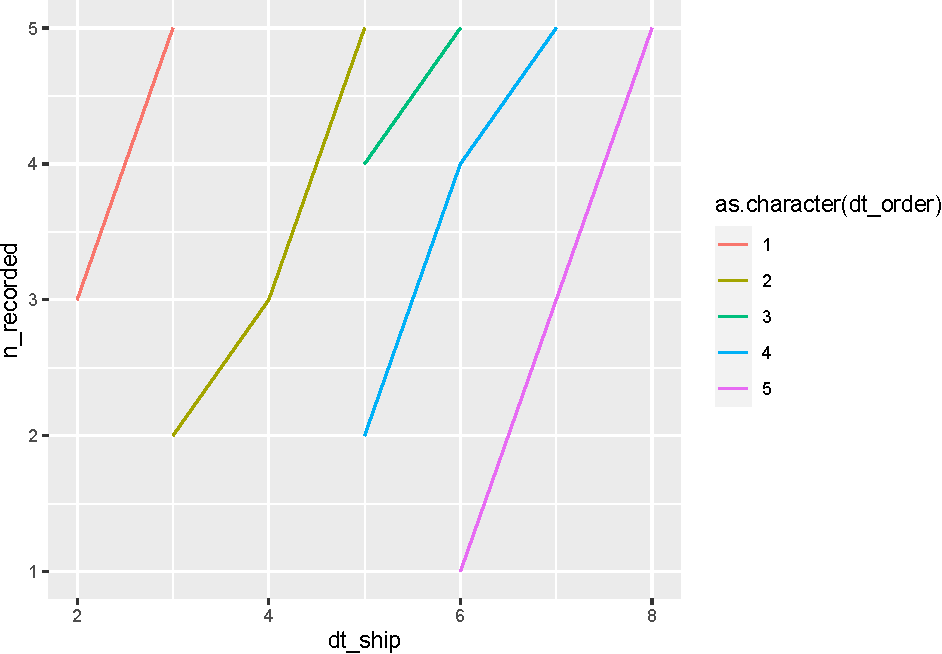
\includegraphics{bookdown_files/figure-latex/unnamed-chunk-20-2.pdf}

\hypertarget{data-transformation-1}{%
\subsection{Data Transformation}\label{data-transformation-1}}

Finally, once the data is roughly where we want it, it likely undergoes many transformations to translate all of the system-generated fields we discussed in data collection into semantically-relevant dimensions for analytical consumers. Of course, the types of transformations that could be done are innumerable with far more variation than data loading. So, we'll just look at a few examples of common failure patterns.

\hypertarget{pre-aggregation-1}{%
\subsubsection{Pre-Aggregation}\label{pre-aggregation-1}}

Data transformations may include aggregating data up to higher levels of granularity for easier analysis. For example, a transformation might add up item-level purchase data to make it easier for an analyst to look at spend per \emph{order} of a specific user.

Data transformations not only transform our data, but they also transform how the dimensions of data quality manifest. If data with some of the \textbf{completeness} or \textbf{uniqueness} issues we discussed with data loading is pre-aggregated, these problems can turn into problems of \textbf{accuracy}. For example, the duplicate or partial data loads that we discussed when aggregated could suggest inaccurately high or low quantities respectively.

\begin{center}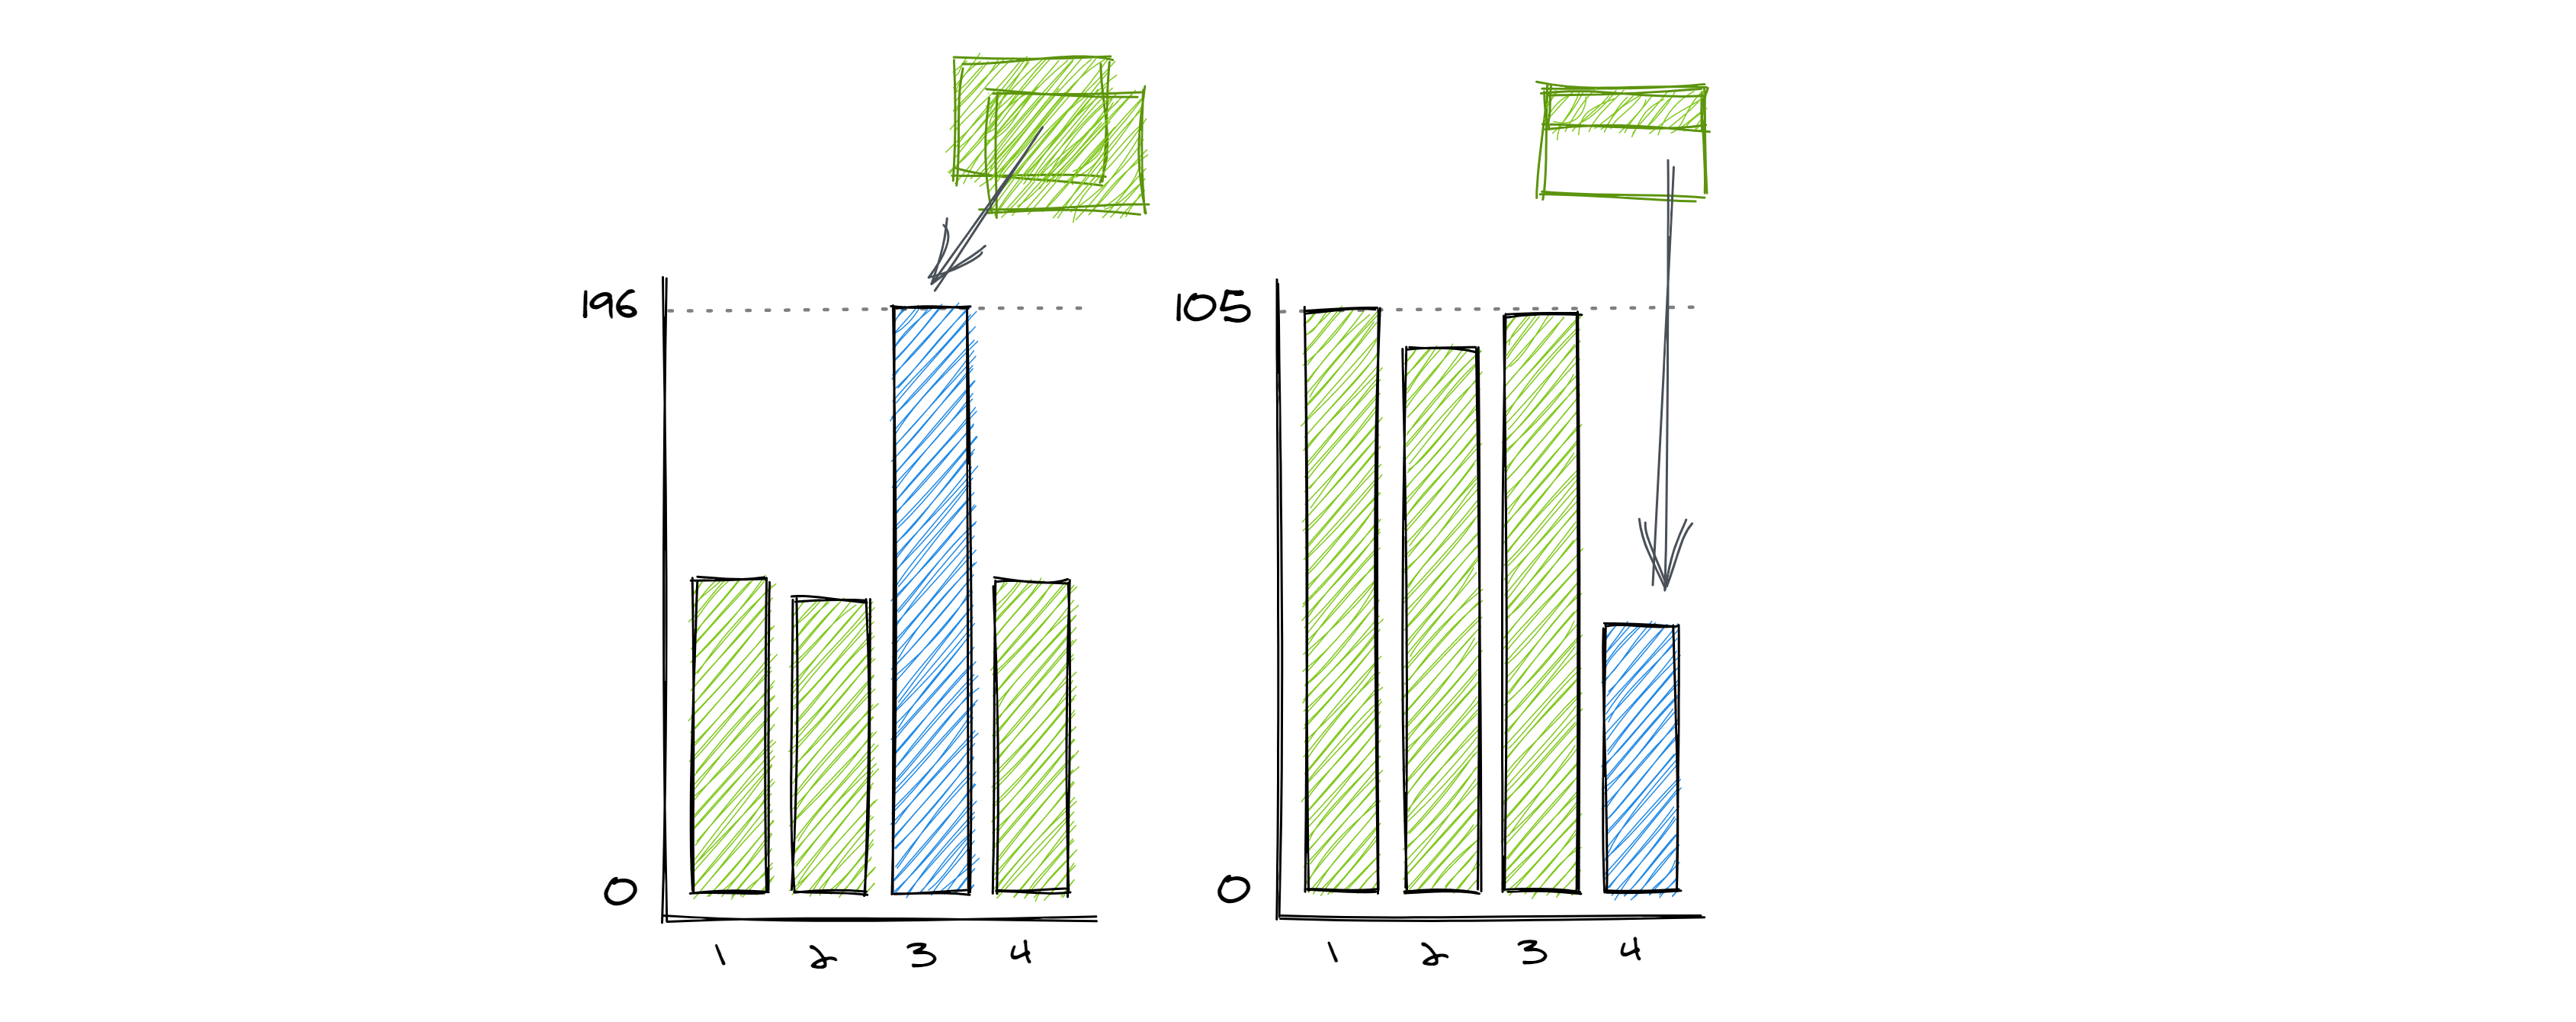
\includegraphics[width=0.9\linewidth]{figures/data-dall/completeness-accuracy} \end{center}

\hypertarget{field-encoding-1}{%
\subsubsection{Field Encoding}\label{field-encoding-1}}

When we assess data consistency across tables,

Categorical fields in a data set might be created in any number of ways including:

\begin{itemize}
\tightlist
\item
  Directly taken from the source
\item
  Coded in a transformation script
\item
  Transformed with logic in a shared user-defined function (\href{https://docs.snowflake.com/en/sql-reference/user-defined-functions.html}{UDFs}) or \href{https://docs.getdbt.com/docs/building-a-dbt-project/jinja-macros/\#macros}{macro}
\item
  Joined from a shared look-up table
\end{itemize}

Each approach has different implications on data consistency and usability.

\begin{center}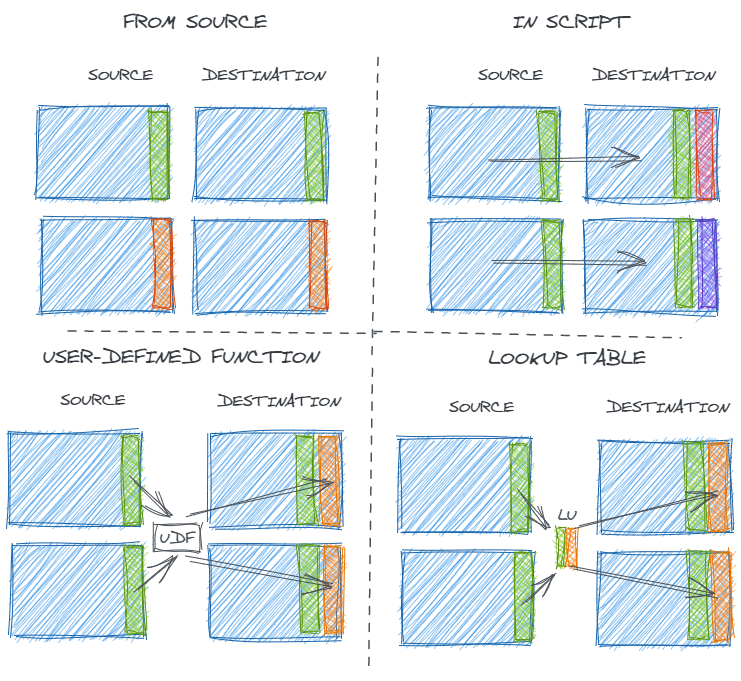
\includegraphics[width=0.9\linewidth]{figures/data-dall/field-encoding} \end{center}

Using fields from the source simply is what it is -- there's no subjectivity or room for manual human error. If multiple tables come from the same source, it's likely but not guaranteed that they will be encoded in the same way.

Coding transformations in the ELT process is easy for data producers. There's no need to coordinate across multiple processes or use cases, and the transformation can be immediately modified when needed. However, that same lack of coordination can lead to different results for fields that should be the same.

Alternatively, macros, UDFs, and look-up tables provided centralized ways to map source data inputs to desired analytical data outputs in a systemic and consistent way. Of course, centralization has its own challenges. If something in the source data changes, the process of updating a centralized UDF or look-up table may be slowed down by the need to seek consensus and collaborate. So, data is more \emph{consistent} but potentially less \emph{accurate}.

Regardless, such engineered values require scrutiny -- paticularly if they are being used as a key to join multiple tables -- and the distinct values in them should be carefully examined.

\hypertarget{updating-transformations-1}{%
\subsubsection{Updating Transformations}\label{updating-transformations-1}}

Of course, data consistency is not only a problem across different data sources but within one data source. Regardless of the method of field encoding used in the previous step, the intersection of data loading and data transformation strategies can introduce data consistency errors over time.

Often, for computation efficiency, analytical tables are loaded using an \emph{incremental} loading strategy. This means that only new records (determined by time period, a set of unique keys, or other criteria) from the upstream source are loaded to the downstream table. This is in contrast to a \emph{full refresh} where the entire downstream table is recreated on each update.

\begin{center}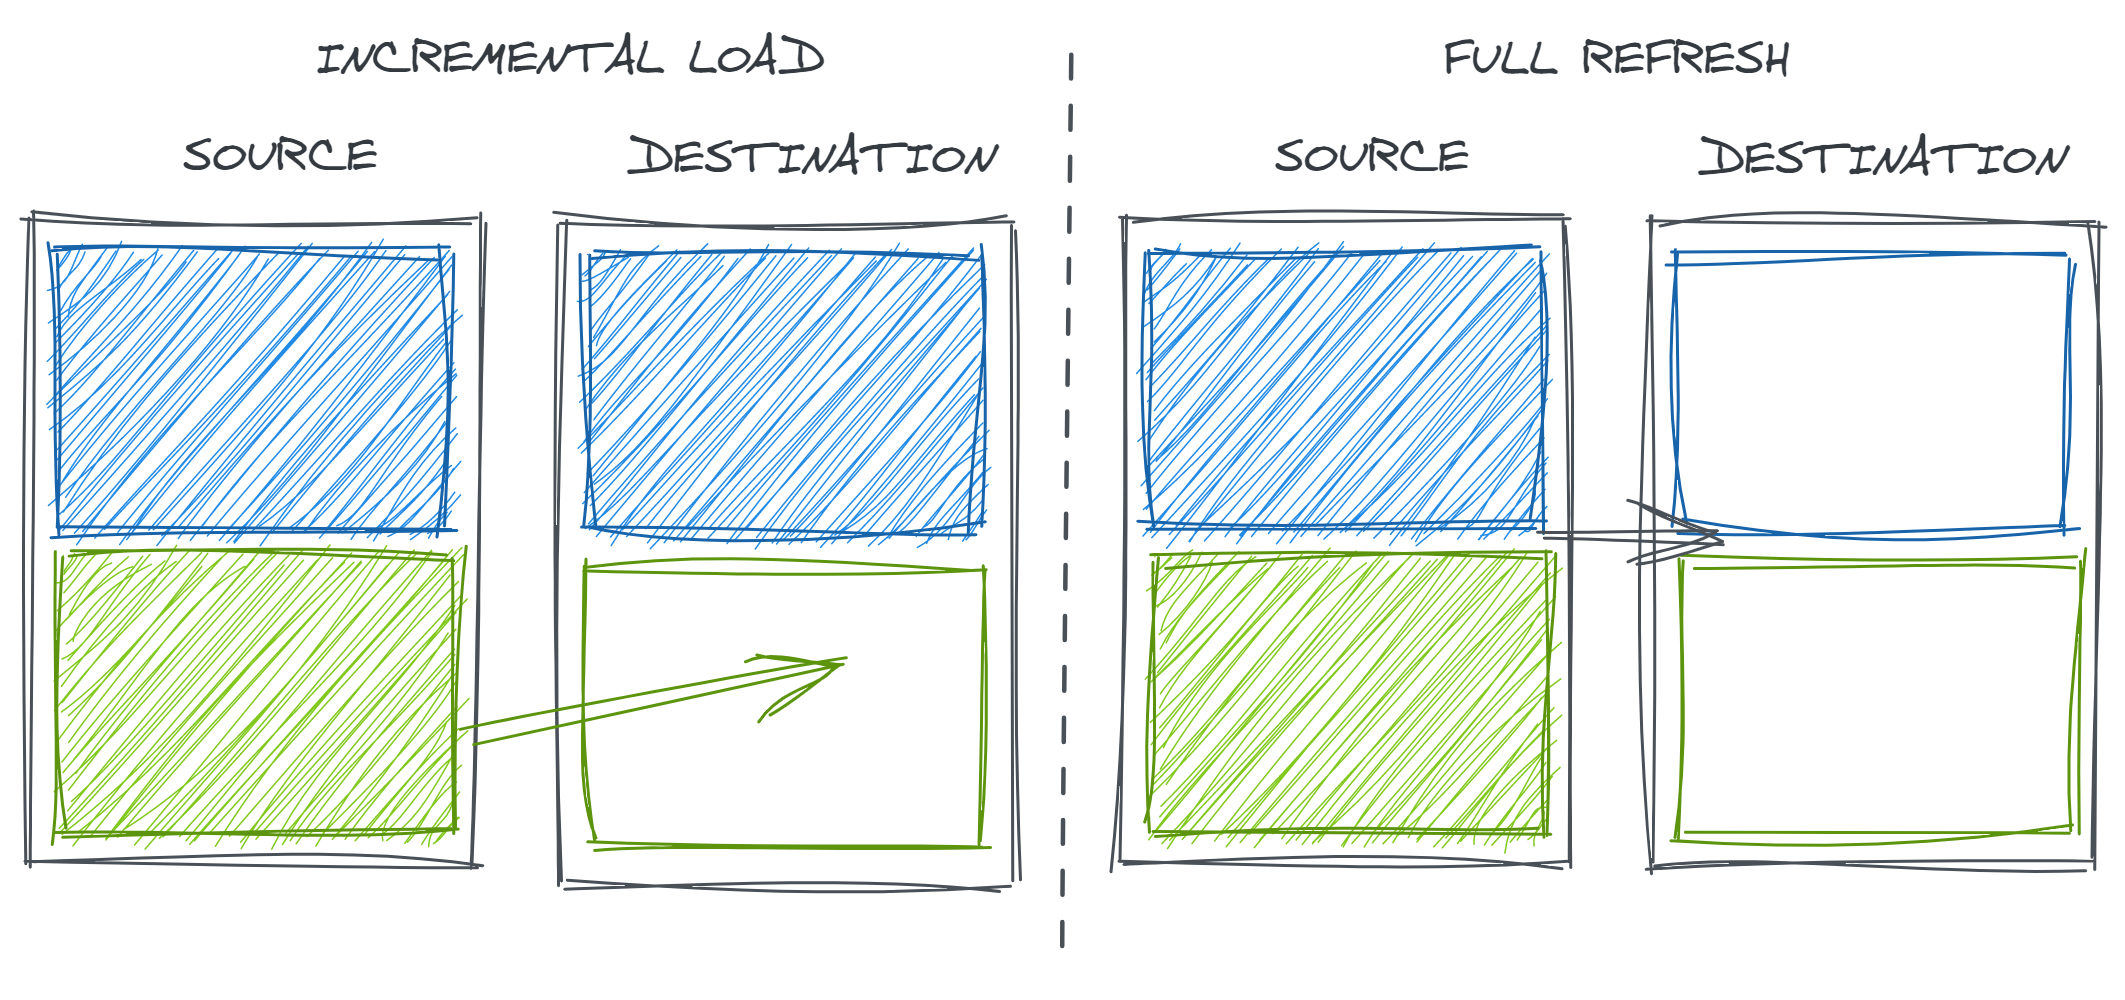
\includegraphics[width=0.9\linewidth]{figures/data-dall/incr-full-good} \end{center}

Incremental loads have many advantages. Rebuilding tables in entirety can be very time consuming and computationally expensive. In particular, in non-cloud data warehouses that are not able to scale computing power on demand, this sort of heavy duty processing job can noticeably drain resources from other queries that are trying to run in the database. Additionally, if the upstream staging data is ephemeral, fully rebuilding the table could mean failing to retain history.

However, in the case that our data transformations change, incremental loads may introduce inconsistency in our data overtime as only new records are created and inserted with the new logic.

\begin{center}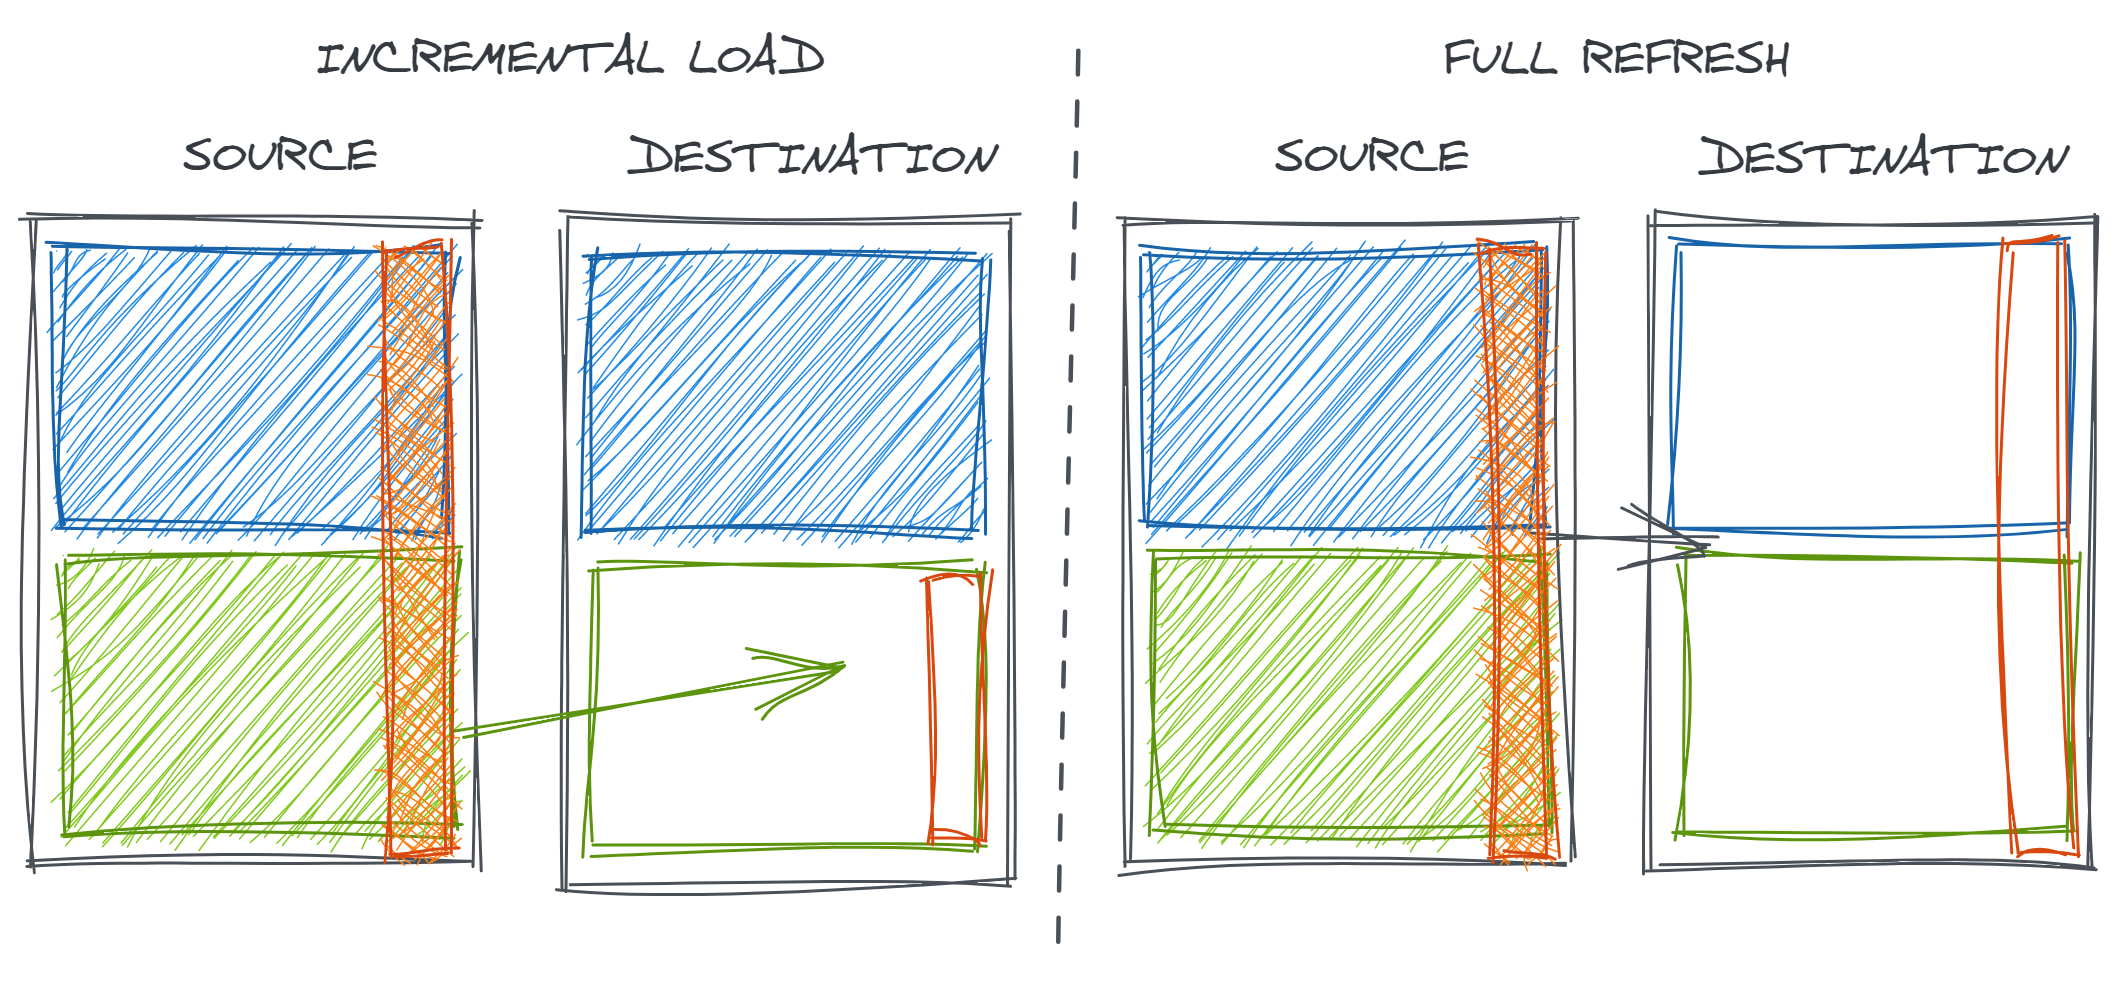
\includegraphics[width=0.9\linewidth]{figures/data-dall/incr-full-bad-col} \end{center}

This is also a problem more broadly if some short-term error is discovered either with data loading or transformation in historical data. Incremental strategies may not always update to include the corrected version of the data.

\begin{center}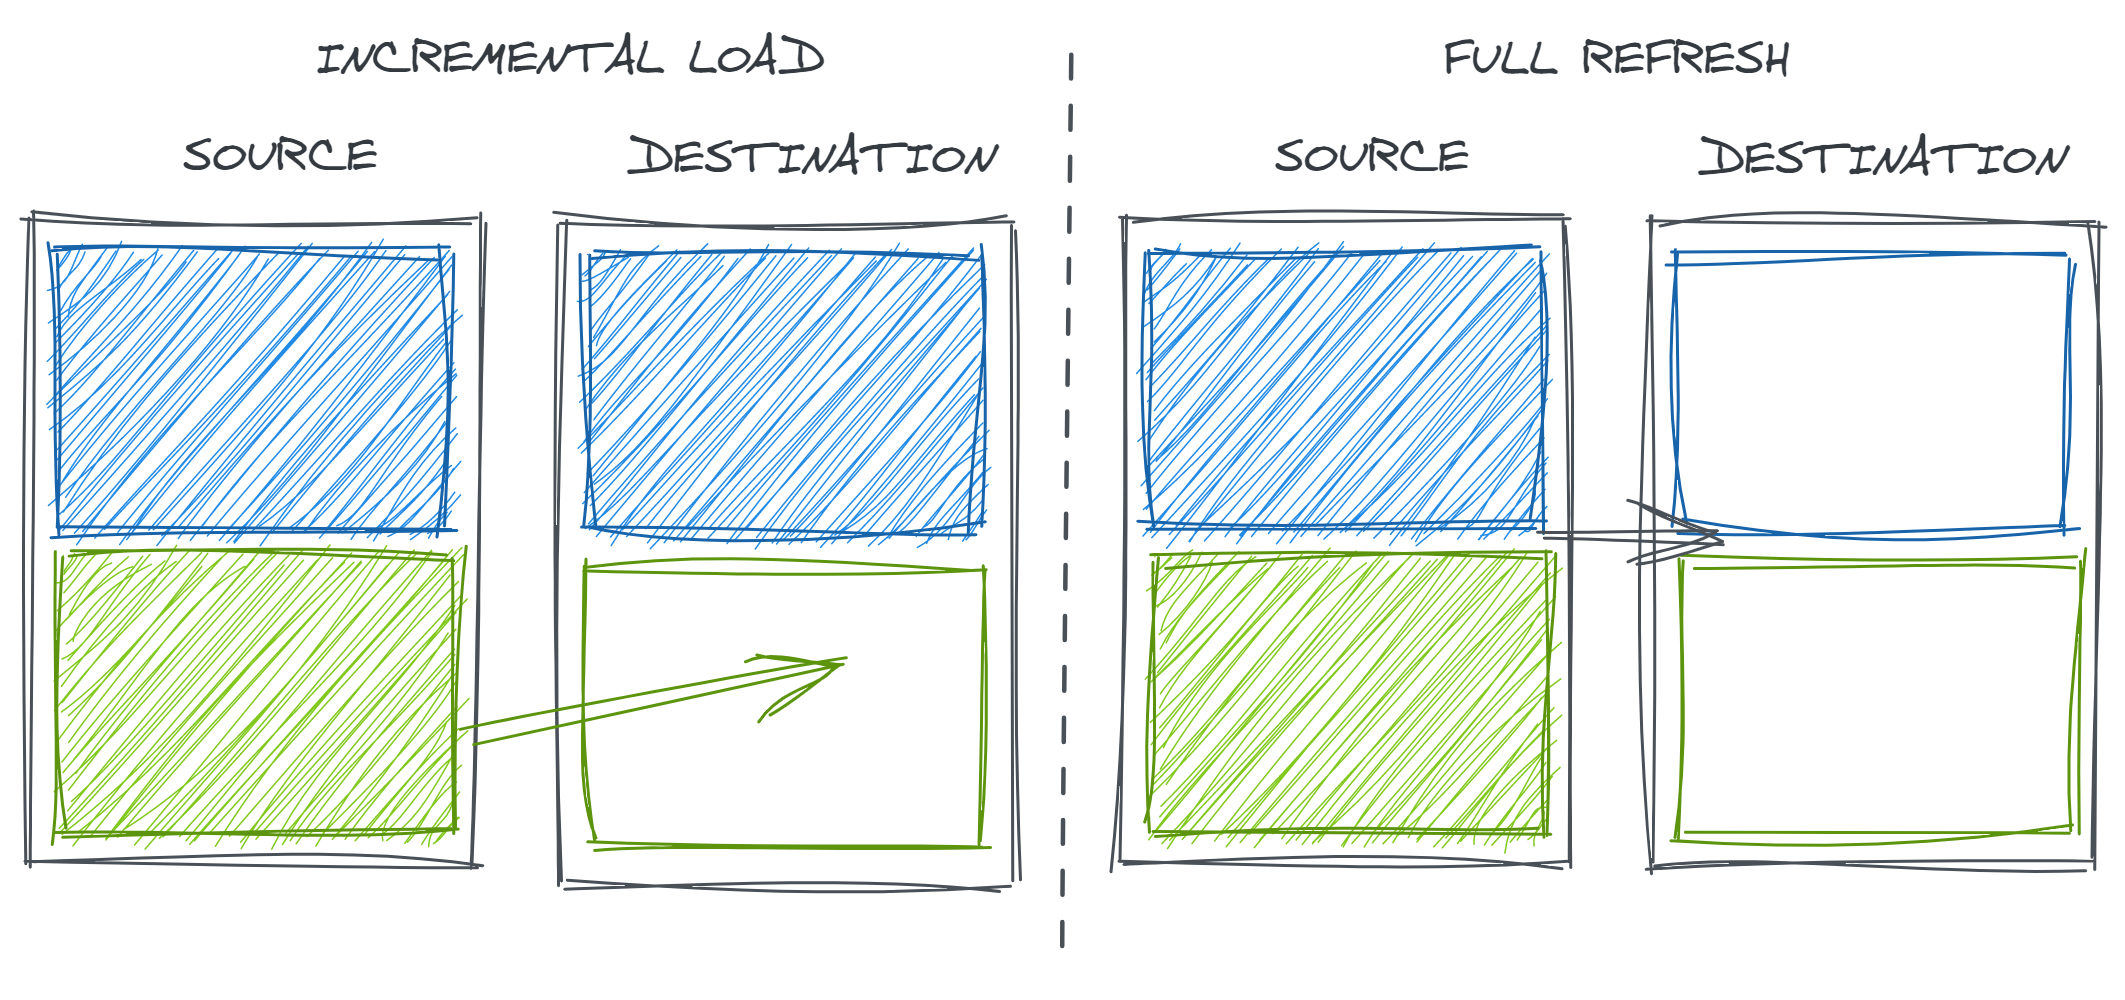
\includegraphics[width=0.9\linewidth]{figures/data-dall/incr-full-good} \end{center}

Regardless, this underscores the need to validate entire datasets and to re-validate when repulling data.

\hypertarget{human-generated-data}{%
\section{Human-Generated Data}\label{human-generated-data}}

Ahhhh

\hypertarget{other-encoding-issues}{%
\section{Other Encoding Issues}\label{other-encoding-issues}}

\begin{itemize}
\tightlist
\item
  for indicators which is 1?
\item
  field values changing over time
\end{itemize}

\hypertarget{strategies}{%
\section{Strategies}\label{strategies}}

--\textgreater{}

\hypertarget{comp-quan}{%
\chapter{Computational Quandaries (WIP)}\label{comp-quan}}

After gaining confidence in one's data (or, at least, making peace with it), the next step in a data analysis is often to start cleaning and exploring that data with summary statistics, plots, and models.
Generally, this requires a computational tool like SQL, R, or python.

The process of computation itself can be fraught with challenges.
Computational tools are extremely literal; they are excellent at doing \emph{precisely what they were told to do} but not often what analysts might have \emph{meant} or \emph{wished} that they would do.
Additionally, the moment an analyst begins to use a tool, the conversation is no longer between them and the data;
suddenly, the mental model of how every single tool developer thought you might want to do analysis affects the tools' behaviors and the analysts' results.

In this chapter, we will explore common ways that tools may do something technically correct, reasonable, and as-intended but very much not what analysts may expect.
Along the way, we will see how computational methods interact with the data encoding choices we discussed in Chapter \ref{data-dall} (Data Dalliances).

\hypertarget{preliminaries---data-computation}{%
\section{Preliminaries - Data Computation}\label{preliminaries---data-computation}}

Before we think about specific tools or failure modes, we can first consider the common types of operations that the analytical tools allow us to do with our data.

\hypertarget{single-table-operations}{%
\subsection{Single Table Operations}\label{single-table-operations}}

Given a single data table, we may wish to do operations (illustrated in Figure \ref{fig:filt-aggr-tran}) such as:

\begin{itemize}
\tightlist
\item
  \textbf{Filtering}: Extracting a subset of a dataset for analysis based on certain inclusion criteria for each record
\item
  \textbf{Aggregation}: Grouping our data table by one or more variables and condensing information across records with \emph{aggregate functions} like counts, sums, and averages
\item
  \textbf{Transformation}: Create new columns or modifying existing columns to represent more complex or domain-specific context
\end{itemize}

\begin{figure}

{\centering 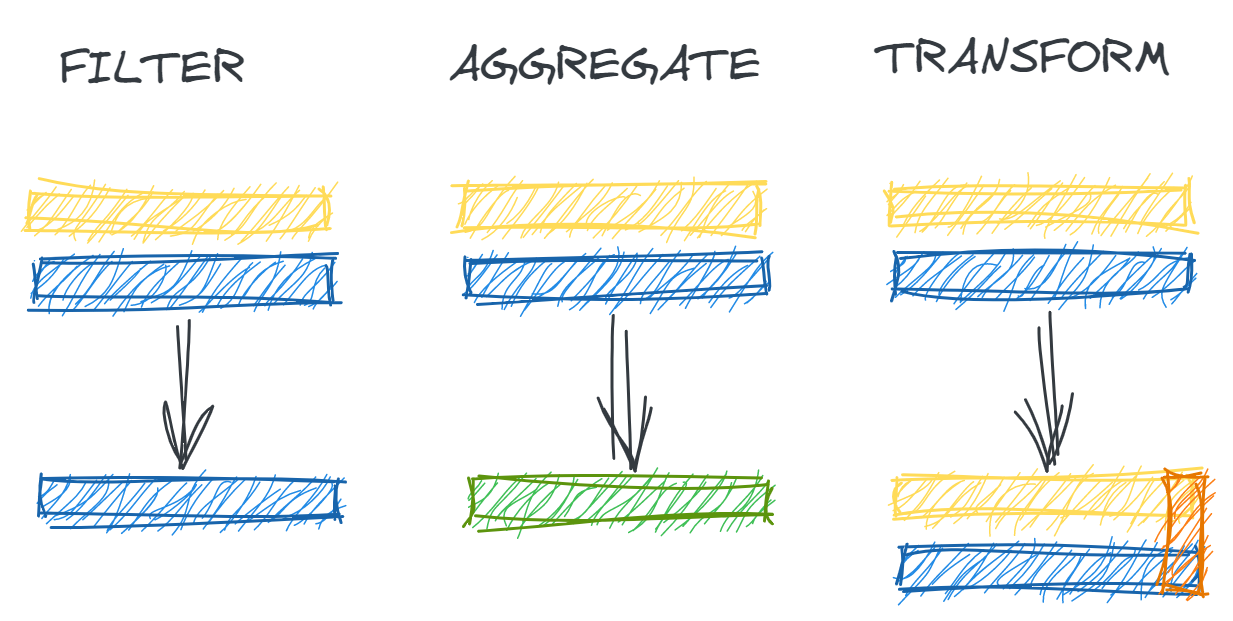
\includegraphics[width=0.9\linewidth]{figures/comp-quan/filt-aggr-tran} 

}

\caption{Illustration of basic single-table data wrangling operations}\label{fig:filt-aggr-tran}
\end{figure}

\hypertarget{multiple-table-operations}{%
\subsection{Multiple Table Operations}\label{multiple-table-operations}}

Often, we can get additional value in an analysis by combining multiple types of information from difference tables.
When working with multiple tables, we may be interested in:

\begin{itemize}
\tightlist
\item
  \textbf{Combining Row-wise}: Taking multiple tables with the same schemas (column names and data types) and creating a single table which contains the union (all records), intersection (only matching), or difference (only in one) of the records in the two tables
\item
  \textbf{Combining Column-wise}: Appending additional fields to existing records through joining (also known as merging) multiple tables
\end{itemize}

\hypertarget{mechanics}{%
\subsection{Mechanics}\label{mechanics}}

All of these operations rely on a few core computational tasks:

\begin{itemize}
\tightlist
\item
  \textbf{Arithmetic}: Basic addition, subtraction, multiplication, and division to aggregate and transform data
\item
  \textbf{Equality}: Comparing whether or not two values are equal is critical for data filtering, column-wise combination, and certain types of data transformation
\item
  \textbf{Casting}: Converting data types of different elements into a comparable format is necessary for row-wise combination and often a prerequisite to certain equality and arithmetic tasks
\end{itemize}

While these operations may seem simple, their behavior within certain tools and when employed for certain data types may sometimes lead to unintuitive or misleading results.

\hypertarget{null-values}{%
\section{Null Values}\label{null-values}}

In Chapter \ref{data-dall} (Data Dalliances), we discuss how null values may represent many different concepts and be encoded in multiple different ways.
In addition to those semantic challenges, various representations of null values may cause different computational problems.\footnote{This problem is not isolated to data analysis tools. For an entertaining example, see the 2019 WIRED article ``How a `NULL' License Plate Landed One Hacker in Ticket Hell'' \citep{barrett} which a real-world software system producing unintended and undesirable behavior when asked to deal with a word \texttt{\textquotesingle{}NULL\textquotesingle{}}.}
In this section, we will explore these potential failure modes.

\hypertarget{types-of-null-values}{%
\subsection{Types of Null Values}\label{types-of-null-values}}

Not only can null values represent many different things (as explored in Chapter \ref{data-dall}), they also may be represented in many different ways. Understanding how nulls are encoded in one's dataset is a critical prerequisite to attempting any of the computations described in the subsequent sections.

\hypertarget{language-representations}{%
\subsubsection{Language representations}\label{language-representations}}

Different programming languages each offer their own versions of null values -- and sometimes more than one. For example, the R language includes \texttt{NA}, typed \texttt{NA}s (e.g.~\texttt{NA\_integer}, \texttt{NA\_character}), \texttt{NaN}, and \texttt{NULL}; meanwhile, core python has \texttt{None} and the \texttt{numpy} module provides a \texttt{nan}.

These different values carry different semantic and functional meanings. For example R's \texttt{NA} generally means ``the presence of an absence'' whereas \texttt{NULL} is ``the absence of a presence''. This is articulated more clearly if we examine the lengths of these objects and observe that \texttt{NA} has a length 1 whereas \texttt{NULL} has a length 0.

\begin{Shaded}
\begin{Highlighting}[]
\FunctionTok{c}\NormalTok{(}\FunctionTok{length}\NormalTok{(}\ConstantTok{NA}\NormalTok{), }\FunctionTok{length}\NormalTok{(}\ConstantTok{NULL}\NormalTok{))}
\end{Highlighting}
\end{Shaded}

\begin{verbatim}
## [1] 1 0
\end{verbatim}

As further proof that these are not interchangeable, we may use the helper functions \texttt{is.na()} and \texttt{is.null()}. It's false that \texttt{NA} is \texttt{NULL} and essentially unable to be evaluated if \texttt{NULL} is \texttt{NA} because \texttt{NULL}s are truly nothing.\footnote{You'll notice that the code chunk below contains four inputs but only three outputs. Why is that? \texttt{is.na(NULL)} returns \texttt{logical(0)}, a zero-length value which cannot be stored in the vector. It's yet another form of missingness!}

\begin{Shaded}
\begin{Highlighting}[]
\FunctionTok{c}\NormalTok{(}
  \FunctionTok{is.na}\NormalTok{(}\ConstantTok{NA}\NormalTok{),}
  \FunctionTok{is.null}\NormalTok{(}\ConstantTok{NULL}\NormalTok{),}
  \FunctionTok{is.na}\NormalTok{(}\ConstantTok{NULL}\NormalTok{),}
  \FunctionTok{is.null}\NormalTok{(}\ConstantTok{NA}\NormalTok{)}
\NormalTok{)}
\end{Highlighting}
\end{Shaded}

\begin{verbatim}
## [1]  TRUE  TRUE FALSE
\end{verbatim}

To further complicate matters, we have \texttt{NaN} (``not a number''), along with \texttt{-Inf} and \texttt{Inf}, which generally arise when we attempt to abuse R's calculator. Somewhat charmingly, \texttt{Inf} and \texttt{-Inf} may be used in some rudimentary calculations where the limit is returned.\footnote{From calculus, we know 1/Inf approaches 0, but Inf/Inf is undefined.}

\begin{Shaded}
\begin{Highlighting}[]
\FunctionTok{c}\NormalTok{(}
  \DecValTok{1}\SpecialCharTok{/}\DecValTok{0}\NormalTok{,   }\CommentTok{\# returns Inf}
  \DecValTok{0}\SpecialCharTok{/}\DecValTok{0}\NormalTok{,   }\CommentTok{\# returns NaN}
  \DecValTok{1}\SpecialCharTok{/}\ConstantTok{Inf}  \CommentTok{\# returns 0}
\NormalTok{)}
\end{Highlighting}
\end{Shaded}

\begin{verbatim}
## [1] Inf NaN   0
\end{verbatim}

\hypertarget{data-encoding-choices-todo}{%
\subsubsection{Data encoding choices (TODO)}\label{data-encoding-choices-todo}}

Beyond these null types offered natively by different programming languages, there are also many different data management \emph{conventions} for null values. Because null values can have many meanings, sometimes missing fields are encoded with ``out of range'' values which intend to suggest a type of missingness.

For example, the US Census Bureau's Medical Expenditure Panel Survey uses the following reserved codes to denote different types of missingness: (TODO: cite p10 \url{https://www.meps.ahrq.gov/data_stats/download_data/pufs/h206a/h206adoc.pdf})

\begin{verbatim}
- -1 INAPPLICABLE Question was not asked due to skip pattern
- -7 REFUSED Question was asked and respondent refused to answer question
- -8 DK Question was asked and respondent did not know answer
- -14 NOT YET TAKEN/USED Respondent answered that the medicine has not yet been used
- -15 CANNOT BE COMPUTED Value cannot be derived from data
\end{verbatim}

This approach preserves a lot of relevant information while, at the same time, being readily apparent that these values are not valid when the data is manually inspect. Unfortunately, manually inspecting every data field is rarely possible, and such sentinel values may go undetected when looking at higher-level summaries.

Consider a survey of a population of retired adults where age is coded as \texttt{999} if not provided. Below, we simulate 100,000 such observations that are uniformly distributed between the age of 65 and 95 (hence, have an expected value of 80). Next, we replace merely \emph{half of a percent} with our ``null'' values of \texttt{999}. Taking the mean with these false values results in a mean of about 85. This number alone might not raise the alarm; after all, we know the dataset's population is older adults. However, accidentally treating these as valid values biases our results by a somewhat remarkable five years.

\begin{Shaded}
\begin{Highlighting}[]
\FunctionTok{set.seed}\NormalTok{(}\DecValTok{123}\NormalTok{)}

\NormalTok{n }\OtherTok{\textless{}{-}} \DecValTok{100000}
\NormalTok{p }\OtherTok{\textless{}{-}} \FloatTok{0.005}
\NormalTok{ages }\OtherTok{\textless{}{-}} \FunctionTok{runif}\NormalTok{(n, }\DecValTok{65}\NormalTok{, }\DecValTok{95}\NormalTok{)}

\NormalTok{ages\_nulls }\OtherTok{\textless{}{-}}\NormalTok{ ages}
\NormalTok{ages\_nulls[}\DecValTok{1}\SpecialCharTok{:}\NormalTok{(n}\SpecialCharTok{*}\NormalTok{p)] }\OtherTok{\textless{}{-}} \DecValTok{999}

\FunctionTok{c}\NormalTok{(}\FunctionTok{mean}\NormalTok{(ages), }\FunctionTok{mean}\NormalTok{(ages\_nulls))}
\end{Highlighting}
\end{Shaded}

\begin{verbatim}
## [1] 79.98 84.57
\end{verbatim}

So, the first order of business with null values is understanding how they are encoded and translation them to the most computationally appropriate form. However, that is only the beginning of the story.

\hypertarget{aggregation}{%
\subsection{Aggregation}\label{aggregation}}

How null values are handled in the simple aggregation of data varies both across different languages and across different functions within a language.
To better understand the problems this might cause, we will look at examples in R and SQL.

To explore aggregation, let's build a simple dataset. We will suppose that we are working with a subscription-based e-commerce service and that we are looking at a \texttt{monthly\_spend} dataset with one record per customer and information about the amount they spent and returned in a given month:

\begin{Shaded}
\begin{Highlighting}[]
\NormalTok{spend }\OtherTok{\textless{}{-}}
  \FunctionTok{data.frame}\NormalTok{(}
    \AttributeTok{AMT\_SPEND =} \FunctionTok{c}\NormalTok{(}\DecValTok{10}\NormalTok{, }\DecValTok{20}\NormalTok{, }\ConstantTok{NA}\NormalTok{),}
    \AttributeTok{AMT\_RETURN =} \FunctionTok{rep}\NormalTok{(}\ConstantTok{NA}\NormalTok{, }\DecValTok{3}\NormalTok{)}
\NormalTok{  )}
\end{Highlighting}
\end{Shaded}

To compute the average amount spent (\texttt{AMT\_SPEND}) with the \texttt{dplyr} package, an analyst might first reasonably write the following \texttt{summarize()} statement.
However, as we can see, due to the presence of null values within the \texttt{AMT\_SPEND} column, the result of this aggregation is for the whole quantity of \texttt{AVG\_SPEND} to be set to the value \texttt{NA}.

A glance at the documentation for the \texttt{mean()} function reveals that it has an \texttt{na.rm} parameter which, when set to true, removes null values from our dataset.
Adding this argument to the previous statement allows us to reach a numerical answer.

\begin{Shaded}
\begin{Highlighting}[]
\FunctionTok{summarize}\NormalTok{(spend, }
          \AttributeTok{AVG\_SPEND =} \FunctionTok{mean}\NormalTok{(AMT\_SPEND),}
          \AttributeTok{AVG\_SPEND\_NARM =} \FunctionTok{mean}\NormalTok{(AMT\_SPEND, }\AttributeTok{na.rm =} \ConstantTok{TRUE}\NormalTok{))}
\end{Highlighting}
\end{Shaded}

\begin{verbatim}
##   AVG_SPEND AVG_SPEND_NARM
## 1        NA             15
\end{verbatim}

However, is this the \emph{right} numerical answer?
What \texttt{na.rm\ =\ TRUE} does is \emph{drop} the null values from the set of numbers being averaged.
However, suppose the null values represent that no purchases were made.
That is, zero dollars were spent.
In effect, we have removed all non-purchasers from the data being averaged.

More precisely, we have switched from taking the average

\[ \frac{ \sum_{1}^{n} Spend }{\sum_{1}^{n} 1} \] over all \(n\) customers

to taking the average

\[ \frac{ \sum_{Spend > 0} Spend }{\sum_{Spend > 0} 1} \] over only those customers with spend

At face value, we could say that the code above is giving the incorrect answer; by dropping some low (zero) purchase amounts, the average amount spend per customer is inflated.
A second perspective, which is someone more philosophically troubling, is that this tiny change to the code which fixed the \emph{obvious} problem (returning a null value) has introduced a \emph{non-obvious} problem by fundamentally changing the question that we are asking.
By dropping all accounts from our table who made no purchases, we are no longer answering ``What is the average amount spent by a new registrant?'' but rather ``What is the average amount spent by an actively engaged customer?''
This technical quirk has significant analytical impact.

To answer the real question at hand, we would instead have a couple of options.
We could manually \texttt{sum()} the amount spent with the option to drop nulls but then divide by the correct denominator (all observations -- not just those with spend) or we could explicitly recode null values in \texttt{AMT\_SPEND} to zero before taking the average.\footnote{Recoding can be done with a number of different general purpose functions like \texttt{ifelse} or \texttt{dplyr::case\_when} in R. Different SQL varaints often offer different options for this purpose with functions such as \texttt{nvl()} or \texttt{zeroifnull()}. A common version across many platforms is \texttt{coalesce()} which takes the first non-null argument listed.}
Either of these options lead to the correct conclusion of a lower average spend amount.

\begin{Shaded}
\begin{Highlighting}[]
\FunctionTok{summarize}\NormalTok{(}
\NormalTok{    spend,}
    \AttributeTok{AVG\_SPEND\_MANUAL =} \FunctionTok{sum}\NormalTok{(AMT\_SPEND, }\AttributeTok{na.rm =} \ConstantTok{TRUE}\NormalTok{) }\SpecialCharTok{/} \FunctionTok{n}\NormalTok{(),}
    \AttributeTok{AVG\_SPEND\_RECODE =} \FunctionTok{mean}\NormalTok{(}\FunctionTok{coalesce}\NormalTok{(AMT\_SPEND, }\DecValTok{0}\NormalTok{))}
\NormalTok{  )}
\end{Highlighting}
\end{Shaded}

\begin{verbatim}
##   AVG_SPEND_MANUAL AVG_SPEND_RECODE
## 1               10               10
\end{verbatim}

This is all well and good if we could just accept that the behaviors above are simply how nulls work, but further complexity comes as we see that there is no industry standard across tools.
For example, as the SQL code below shows, SQL's \texttt{avg()} function behaves more like R's \texttt{mean()} \emph{with} the \texttt{na.rm\ =\ TRUE} option set.
That is, the default behavior of SQL is to only operate on the valid and available values.

\begin{Shaded}
\begin{Highlighting}[]
\KeywordTok{SELECT} \FunctionTok{avg}\NormalTok{(amt\_spend) }\KeywordTok{as}\NormalTok{ AVG\_SPEND}
\KeywordTok{FROM}\NormalTok{ spend}
\end{Highlighting}
\end{Shaded}

\begin{verbatim}
##   AVG_SPEND
## 1        15
\end{verbatim}

However, this is not to suggest that null values cannot also be destructive in SQL.
While aggregation functions (which compute over the \emph{rows/records}) like \texttt{sum()} and \texttt{avg()} drop nulls, operators like \texttt{+} and \texttt{-} (which compute \emph{across columns/variables} in the \emph{same row/record}) do not exhibit the same behavior.
Consider, for example, if we wish to calculate the average net purchase amount (purchases minus returns) instead of the gross (total) purchase amount.

\begin{Shaded}
\begin{Highlighting}[]
\KeywordTok{SELECT} \FunctionTok{avg}\NormalTok{(amt\_spend}\OperatorTok{{-}}\NormalTok{amt\_return) }\KeywordTok{as}\NormalTok{ AVG\_SPEND\_NET}
\KeywordTok{FROM}\NormalTok{ spend}
\end{Highlighting}
\end{Shaded}

\begin{verbatim}
##   AVG_SPEND_NET
## 1            NA
\end{verbatim}

Despite what we learned above about SQL's \texttt{avg()} function, the query above returns only a null value.
What has happened?
In our \texttt{spend} dataset, the \texttt{amt\_return} column is completely null (representing no returns).
Because the subtraction occurs before the average is taken, subtracting real numbers in \texttt{amt\_spend} with null values in \texttt{amt\_return} creates a column of all null values which are then fed into the \texttt{avg()} function.
This process is shown step-by-step below.

\begin{Shaded}
\begin{Highlighting}[]
\KeywordTok{SELECT}
\NormalTok{  amt\_spend, }
\NormalTok{  amt\_return, }
\NormalTok{  amt\_spend}\OperatorTok{{-}}\NormalTok{amt\_return }
\KeywordTok{FROM}\NormalTok{ spend}
\end{Highlighting}
\end{Shaded}

\begin{verbatim}
##   AMT_SPEND AMT_RETURN amt_spend-amt_return
## 1        10         NA                   NA
## 2        20         NA                   NA
## 3        NA         NA                   NA
\end{verbatim}

\hypertarget{comparison}{%
\subsection{Comparison}\label{comparison}}

Null values don't just introduce complexity when doing arithmetic. Difficulties also arise any time multiple variables are assessed for equality or inequality. Since a null value is unknown, most programming languages generally will \emph{not} consider nulls to be comparable with other nulls.

We can simple examples of this in both R and SQL.

\begin{Shaded}
\begin{Highlighting}[]
\FunctionTok{c}\NormalTok{(}
  \ConstantTok{NA} \SpecialCharTok{==} \DecValTok{3}\NormalTok{, }
  \ConstantTok{NA} \SpecialCharTok{\textgreater{}} \DecValTok{10}\NormalTok{, }
  \ConstantTok{NA} \SpecialCharTok{==} \ConstantTok{NA}
\NormalTok{  )}
\end{Highlighting}
\end{Shaded}

\begin{verbatim}
## [1] NA NA NA
\end{verbatim}

\begin{Shaded}
\begin{Highlighting}[]
\KeywordTok{SELECT}
\NormalTok{  (}\KeywordTok{NULL} \OperatorTok{=} \DecValTok{3}\NormalTok{) }\KeywordTok{as}\NormalTok{ NULL\_EQ\_NUM,}
\NormalTok{  (}\KeywordTok{NULL} \OperatorTok{\textgreater{}} \DecValTok{10}\NormalTok{) }\KeywordTok{as}\NormalTok{ NULL\_GT\_NUM,}
\NormalTok{  (}\KeywordTok{NULL} \OperatorTok{=} \KeywordTok{NULL}\NormalTok{) }\KeywordTok{as}\NormalTok{ NULL\_EQ\_NULL}
\end{Highlighting}
\end{Shaded}

\begin{verbatim}
##   NULL_EQ_NUM NULL_GT_NUM NULL_EQ_NULL
## 1          NA          NA           NA
\end{verbatim}

In these toy examples, such outcomes may seem perfectly logical.
However, this same reasoning can arise in sneakier ways and lead to uninteded results when equality evaluations are \emph{implicit} in the task at hand instead of the singular focus.
We'll now see examples from data filtering, joining, and transformation.

\hypertarget{filtering}{%
\subsubsection{Filtering}\label{filtering}}

Suppose we want to split our dataset into two datasets based on high or low values of spend.
We might assume the following two lines of code will create a clear partition\footnote{A \textbf{paritition} of our data would imply that every record is contained in precisely one group} of results.

\begin{Shaded}
\begin{Highlighting}[]
\NormalTok{spend\_lt20 }\OtherTok{\textless{}{-}} \FunctionTok{filter}\NormalTok{(spend, AMT\_SPEND }\SpecialCharTok{\textless{}} \DecValTok{20}\NormalTok{)}
\NormalTok{spend\_gte20 }\OtherTok{\textless{}{-}} \FunctionTok{filter}\NormalTok{(spend, AMT\_SPEND }\SpecialCharTok{\textgreater{}=} \DecValTok{20}\NormalTok{)}
\end{Highlighting}
\end{Shaded}

However, examining the resulting datasets, we see than \emph{neither} contains the null records.

\begin{Shaded}
\begin{Highlighting}[]
\NormalTok{spend\_lt20}
\end{Highlighting}
\end{Shaded}

\begin{verbatim}
##   AMT_SPEND AMT_RETURN
## 1        10         NA
\end{verbatim}

\begin{Shaded}
\begin{Highlighting}[]
\NormalTok{spend\_gte20}
\end{Highlighting}
\end{Shaded}

\begin{verbatim}
##   AMT_SPEND AMT_RETURN
## 1        20         NA
\end{verbatim}

The same situation results in SQL.

\begin{Shaded}
\begin{Highlighting}[]
\KeywordTok{SELECT} \OperatorTok{*}
\KeywordTok{FROM}\NormalTok{ spend}
\KeywordTok{WHERE}\NormalTok{ AMT\_SPEND }\OperatorTok{\textless{}} \DecValTok{20}
\end{Highlighting}
\end{Shaded}

\begin{verbatim}
##   AMT_SPEND AMT_RETURN
## 1        10         NA
\end{verbatim}

\begin{Shaded}
\begin{Highlighting}[]
\KeywordTok{SELECT} \OperatorTok{*}
\KeywordTok{FROM}\NormalTok{ spend}
\KeywordTok{WHERE}\NormalTok{ AMT\_SPEND }\OperatorTok{\textgreater{}=} \DecValTok{20}
\end{Highlighting}
\end{Shaded}

\begin{verbatim}
##   AMT_SPEND AMT_RETURN
## 1        20         NA
\end{verbatim}

Thus, whenever our data has null values, the very common act of data filtering risks excluding important information.

\hypertarget{joining}{%
\subsubsection{Joining}\label{joining}}

The same phenomenon as described above also happens when joining multiple datasets.

Suppose we have multiple datasets we wish to merge based on columns denoting a record's name and date of birthday.
For ease of exploration, we will make the simplest possible such dataset and simply try to merge it to itself.
(This may seem silly, but often when trying to understand \emph{computationally} complex things, it is a good idea to make the scenario as simple as possible.
In fact, this idea is core to the concept of computational unit tests which we will discuss at the end of this chapter.)

\begin{Shaded}
\begin{Highlighting}[]
\NormalTok{bday }\OtherTok{\textless{}{-}} \FunctionTok{data.frame}\NormalTok{(}\AttributeTok{NAME =} \FunctionTok{c}\NormalTok{(}\StringTok{\textquotesingle{}Anne\textquotesingle{}}\NormalTok{, }\StringTok{\textquotesingle{}Bob\textquotesingle{}}\NormalTok{), }\AttributeTok{BIRTHDAY =} \FunctionTok{c}\NormalTok{(}\StringTok{\textquotesingle{}2000{-}01{-}01\textquotesingle{}}\NormalTok{, }\ConstantTok{NA}\NormalTok{))}
\NormalTok{bday}
\end{Highlighting}
\end{Shaded}

\begin{verbatim}
##   NAME   BIRTHDAY
## 1 Anne 2000-01-01
## 2  Bob       <NA>
\end{verbatim}

In SQL, if we try to join this table, the records in row 1 will match because \texttt{\textquotesingle{}Anne\textquotesingle{}\ ==\ \textquotesingle{}Anne\textquotesingle{}} and \texttt{\textquotesingle{}2000-01-01\textquotesingle{}\ ==\ \textquotesingle{}2000-01-01\textquotesingle{}}.
However, poor Bob's record is eliminated because his birthdate is logged as null, and \texttt{NA\ ==\ NA} is false.

\begin{Shaded}
\begin{Highlighting}[]
\KeywordTok{SELECT}\NormalTok{ a.}\OperatorTok{*}
\KeywordTok{FROM}
\NormalTok{  bday }\KeywordTok{as}\NormalTok{ a}
  \KeywordTok{INNER} \KeywordTok{JOIN}
\NormalTok{  bday }\KeywordTok{as}\NormalTok{ b}
  \KeywordTok{ON}
\NormalTok{  a.NAME }\OperatorTok{=}\NormalTok{ b.NAME }\KeywordTok{and}
\NormalTok{  a.BIRTHDAY }\OperatorTok{=}\NormalTok{ b.BIRTHDAY}
\end{Highlighting}
\end{Shaded}

\begin{verbatim}
##   NAME   BIRTHDAY
## 1 Anne 2000-01-01
\end{verbatim}

In contrast, R's \texttt{dplyr::inner\_join()} function will not do this by default.
This function lets us specifically control how nulls are matches with the \texttt{na\_matches} argument, with a default option to match on \texttt{NA} values.
(You may read more about the argument by typing \texttt{?dplyr::inner\_join} in the R console to pull up the documentation.)

\begin{Shaded}
\begin{Highlighting}[]
\FunctionTok{inner\_join}\NormalTok{(bday, bday, }\AttributeTok{by =} \FunctionTok{c}\NormalTok{(}\StringTok{\textquotesingle{}NAME\textquotesingle{}}\NormalTok{, }\StringTok{\textquotesingle{}BIRTHDAY\textquotesingle{}}\NormalTok{))}
\end{Highlighting}
\end{Shaded}

\begin{verbatim}
##   NAME   BIRTHDAY
## 1 Anne 2000-01-01
## 2  Bob       <NA>
\end{verbatim}

This example then is not only a cautionary tale for how null values may unintentionally corrupt our data transformations but also how ``brittle'' our knowledge and intuition may be when moving between tools.
Neither of these default behaviors is strictly better or worse, but they are definitely different and have real implications on our analysis.

\hypertarget{transformation}{%
\subsubsection{Transformation}\label{transformation}}

A common task in data analysis is to aggregate results by subgroup.
For example, we might want to summarize how many customers (rows/records) spent more or less than \$10. To discern this, we might create a categorical variable for high versus low purchase amounts, group by this variable and count.

The psuedocode would read something like this:

\begin{Shaded}
\begin{Highlighting}[]
\NormalTok{data }\SpecialCharTok{\%\textgreater{}\%}
  \FunctionTok{mutate}\NormalTok{(}\AttributeTok{HIGH\_LOW =} \SpecialCharTok{\textless{}}\ErrorTok{\textless{}}\NormalTok{ transform AMT\_SPEND }\SpecialCharTok{\textgreater{}}\ErrorTok{\textgreater{}}\NormalTok{) }\SpecialCharTok{\%\textgreater{}\%}
  \FunctionTok{group\_by}\NormalTok{(HIGH\_LOW) }\SpecialCharTok{\%\textgreater{}\%}
  \FunctionTok{count}\NormalTok{()}
\end{Highlighting}
\end{Shaded}

To define the \texttt{HIGH\_LOW} variable, we might use a function like \texttt{ifelse()}, \texttt{dplyr::if\_else()}, or \texttt{dplyr::case\_when()}.
However, once again, we have the issue of how values are \emph{partitioned} when nulls are included.
If we recode any records with \texttt{AMT\_SPEND} of less than or equal to 10 to ``Low'' and default the rest to ``High'', we will accidentally count all null values in the ``High'' group.

\begin{Shaded}
\begin{Highlighting}[]
\NormalTok{spend }\SpecialCharTok{\%\textgreater{}\%}
  \FunctionTok{mutate}\NormalTok{(}\AttributeTok{HIGH\_LOW =} \FunctionTok{case\_when}\NormalTok{(}
\NormalTok{    AMT\_SPEND }\SpecialCharTok{\textless{}=} \DecValTok{10} \SpecialCharTok{\textasciitilde{}} \StringTok{"Low"}\NormalTok{, }
    \ConstantTok{TRUE} \SpecialCharTok{\textasciitilde{}} \StringTok{"High"}\NormalTok{)}
\NormalTok{    ) }\SpecialCharTok{\%\textgreater{}\%}
  \FunctionTok{group\_by}\NormalTok{(HIGH\_LOW) }\SpecialCharTok{\%\textgreater{}\%} 
  \FunctionTok{count}\NormalTok{()}
\end{Highlighting}
\end{Shaded}

\begin{verbatim}
## # A tibble: 2 x 2
## # Groups:   HIGH_LOW [2]
##   HIGH_LOW     n
##   <chr>    <int>
## 1 High         2
## 2 Low          1
\end{verbatim}

Instead, it is more accurate and transparent (unless we know specifically what null values mean and what group they should be part of) to not let one of our ``core'' categories by the ``default'' case in our logic.
We can explicitly encode any residual values as something like ``OTHER'' or ``ERROR'' to help us see that there is a problem requiring extra attention.

\begin{Shaded}
\begin{Highlighting}[]
\NormalTok{spend }\SpecialCharTok{\%\textgreater{}\%}
  \FunctionTok{mutate}\NormalTok{(}\AttributeTok{HIGH\_LOW =} \FunctionTok{case\_when}\NormalTok{(}
\NormalTok{    AMT\_SPEND }\SpecialCharTok{\textless{}=} \DecValTok{10} \SpecialCharTok{\textasciitilde{}} \StringTok{"Low"}\NormalTok{, }
\NormalTok{    AMT\_SPEND }\SpecialCharTok{\textgreater{}} \DecValTok{10} \SpecialCharTok{\textasciitilde{}} \StringTok{"High"}\NormalTok{,}
    \ConstantTok{TRUE} \SpecialCharTok{\textasciitilde{}} \StringTok{"OTHER"}\NormalTok{)}
\NormalTok{    ) }\SpecialCharTok{\%\textgreater{}\%}
  \FunctionTok{group\_by}\NormalTok{(HIGH\_LOW) }\SpecialCharTok{\%\textgreater{}\%} 
  \FunctionTok{count}\NormalTok{()}
\end{Highlighting}
\end{Shaded}

\begin{verbatim}
## # A tibble: 3 x 2
## # Groups:   HIGH_LOW [3]
##   HIGH_LOW     n
##   <chr>    <int>
## 1 High         1
## 2 Low          1
## 3 OTHER        1
\end{verbatim}

\hypertarget{strings-wip}{%
\section{Strings (WIP)}\label{strings-wip}}

String data can be inherently appealing. At their best, strings are used to bring more readable and human interpretable values into a dataset. However, string data and the processing thereof comes with its own challenges.

First, unlike numbers, human language strings can be ambiguously defined. \texttt{2} is the only number to represent the value of two. However, the incorporation of human language means that many different words, phrases, and formatting choices can represent the same concept. This is confounded by instances where string data was manually entered, as is the case with user-input data.\footnote{I can accurately say my name is ``Emily'', ``Emily Riederer'', ``Emily E. Riederer'', ``Ms.~Emily Riederer''. Additionally, if I spell my name over the phone, I can likely end up ``Emily Rieder'' or if I type it and mindlessly accept autocorrect, I'm ``Emily Reindeer''. This inconsistently may be problematic if you are trying to combine my data across different sources where I provided my name in different ways.}

Secondly, string data is one of the most flexible datatypes and can contain any other types of information -- from should-be-logical values (\texttt{"yes"/"no"}, \texttt{"true"/"false"}), should-be-numeric values (\texttt{"27"}), should-be-date values (\texttt{"2020-01-01"}), and even complex data encodings like JSON blobs (\texttt{"\{"name":\{"first":"emily","last":"riederer"\},"social":\{"twitter":"emilyriederer","github":"emilyriederer","linkedin":"emilyriederer"\}\}"} with hideous formatting for emphasis.) For a data publisher, this may be a convenience, but as we will see it can turn into a frustration or a liability when functions and comparison operations are attempted with strings that semantically represent a different type of value.

\hypertarget{dirty-strings}{%
\subsection{Dirty Strings}\label{dirty-strings}}

whitespace

\begin{Shaded}
\begin{Highlighting}[]
\StringTok{"a"} \SpecialCharTok{==} \StringTok{"a"}
\StringTok{"a b"} \SpecialCharTok{==} \StringTok{"a b"}
\StringTok{"a b"} \SpecialCharTok{==} \StringTok{"a  b"}
\StringTok{"a b"} \SpecialCharTok{==} \StringTok{"a b "}
\end{Highlighting}
\end{Shaded}

\begin{verbatim}
## [1] TRUE
## [1] TRUE
## [1] FALSE
## [1] FALSE
\end{verbatim}

``fancy'' characters (alternate encodings like ms word)

\begin{Shaded}
\begin{Highlighting}[]
\StringTok{\textquotesingle{} " \textquotesingle{}} \SpecialCharTok{==} \StringTok{\textquotesingle{} " \textquotesingle{}}
\StringTok{\textquotesingle{} “ \textquotesingle{}} \SpecialCharTok{==} \StringTok{\textquotesingle{} " \textquotesingle{}}
\end{Highlighting}
\end{Shaded}

\begin{verbatim}
## [1] TRUE
## [1] FALSE
\end{verbatim}

special characters and display versus values

\begin{Shaded}
\begin{Highlighting}[]
\NormalTok{x }\OtherTok{\textless{}{-}} \StringTok{"a}\SpecialCharTok{\textbackslash{}t}\StringTok{b"}
\FunctionTok{cat}\NormalTok{(x) }\CommentTok{\# what you see...}
\NormalTok{x }\SpecialCharTok{==} \StringTok{"a    b"} \CommentTok{\# ...is not what you get}
\end{Highlighting}
\end{Shaded}

\begin{verbatim}
## a    b[1] FALSE
\end{verbatim}

\hypertarget{regular-expressions-todo}{%
\subsection{Regular Expressions (TODO)}\label{regular-expressions-todo}}

we promised not to be solution oriented, but

\emph{not} knowing regex is a disaster when trying to work with string data\ldots{}

\hypertarget{comparison-1}{%
\subsection{Comparison}\label{comparison-1}}

TODO

\hypertarget{string-ordering}{%
\subsubsection{String ordering}\label{string-ordering}}

Strings are ranked based on \emph{alphabetical order} just like a dictionary. Some properties of this ordering include that:

\begin{itemize}
\tightlist
\item
  numbers are smaller than letters (\texttt{1\ \textless{}\ "a"})
\item
  lower-case is smaller than upper case (\texttt{"a"\ \textless{}\ "A"})
\item
  fewer characters are smaller than more characters (\texttt{"a"\ \textless{}\ "aa"})
\end{itemize}

Such rules make perfect sense for true characters. However, when strings are used as a ``catch all'' to represent other structures, typical comparison operators can produce odd results. For example, its generally uncontroverisal that ninety-one is less than one hundred twenty. However, the string \texttt{"91"} is \emph{greater than} \texttt{"120"} because only the chacter \texttt{"9"} is compared to the character \texttt{"1"}.\footnote{Similarly, \texttt{"91"\ \textgreater{}\ "905"} because since they both start with 9, we move on to compare 1 which is greater than 0.}

\begin{Shaded}
\begin{Highlighting}[]
\DecValTok{91} \SpecialCharTok{\textless{}} \DecValTok{120}
\StringTok{"91"} \SpecialCharTok{\textless{}} \StringTok{"120"}
\end{Highlighting}
\end{Shaded}

\begin{verbatim}
## [1] TRUE
## [1] FALSE
\end{verbatim}

When strings are used to represent strings, comparison operators may or may not work depending on the precise formatting convertions. Below, we see that ``YYYYQQ''-formats sort correctly because the information is hierarchically nested; millenia are compared before centuries, centuries before decades, decades before years, and years before quarters. However, many other string representations of dates, like ``QQ-YYYY'' will not order correctly. Related topics will be discussed in the ``Dates and Times'' section.

\begin{Shaded}
\begin{Highlighting}[]
\StringTok{"20190Q4"} \SpecialCharTok{\textless{}} \StringTok{"2020Q3"} \CommentTok{\# string (alphabetic) ordering same as semantic ordering}
\StringTok{"Q4{-}2019"} \SpecialCharTok{\textless{}} \StringTok{"Q3{-}2020"} \CommentTok{\# string and semantic orderings are different}
\end{Highlighting}
\end{Shaded}

\begin{verbatim}
## [1] TRUE
## [1] FALSE
\end{verbatim}

These examples demonstrate that we shouldn't rely on sorting schemes that follow different rules. Before doing comparisons on such types, its a safer bet to cast them to the format most truly representative of their types. If, for some reason, you do wish to keep them as strings, the second example shows that its is wise to format them in the most conducive format possible so things just work.

\hypertarget{type-coercion}{%
\subsubsection{Type coercion}\label{type-coercion}}

We discussed string comparison before when looking at ``dirty'' strings. More unexpected behavior arises when strings are compared across different data types. Many computing programs will attempt to \emph{coerce} the objects to a similar and comparable type. Sometimes, this can be handy as operations ``just work'', but as always there is a cost for convenience. As we'll see, delegating important decisions to our computing engine may not always capture the semantic relationships that we are most interested in.

For example, consider compare a string and a number. To make them more comparable, R will convert them both to strings before checking for equality. Thus, the number \texttt{2020} is equivalent to the string \texttt{"2020"} but not the string \texttt{"02020"}.

\begin{Shaded}
\begin{Highlighting}[]
\StringTok{"2020"} \SpecialCharTok{==} \DecValTok{2020}
\StringTok{"02020"} \SpecialCharTok{==} \DecValTok{2020}
\end{Highlighting}
\end{Shaded}

\begin{verbatim}
## [1] TRUE
## [1] FALSE
\end{verbatim}

In constrast, SQLite\footnote{Different versions of SQL may differ} thinks that the string \texttt{\textquotesingle{}2020\textquotesingle{}} is greater than the number 2020 and that these two quantities are not equal.

\begin{Shaded}
\begin{Highlighting}[]
\FunctionTok{sqldf}\NormalTok{(}\StringTok{"select }
\StringTok{      case when \textquotesingle{}2020\textquotesingle{} = 2020 then 1 else 0 end as is\_eq,}
\StringTok{      case when not \textquotesingle{}2020\textquotesingle{} == 2020 then 1 else 0 end as not\_eq,}
\StringTok{      case when \textquotesingle{}2020\textquotesingle{} \textless{} 2020 then 1 else 0 end as is\_lt,}
\StringTok{      case when \textquotesingle{}2020\textquotesingle{} \textgreater{} 2020 then 1 else 0 end as is\_gt}
\StringTok{      "}\NormalTok{)}
\end{Highlighting}
\end{Shaded}

\begin{verbatim}
##   is_eq not_eq is_lt is_gt
## 1     0      1     0     1
\end{verbatim}

\^{}TODO: where this could cause problems (FIPS example?)

\hypertarget{dates-and-times-wip}{%
\section{Dates and Times (WIP)}\label{dates-and-times-wip}}

Unlike character strings, dates and times seem like they should be well defined with distinct, quantifiable components like years, months, and days. However, many different conventions for date formatting and underlying storage formats exist. This leads to similar challenges with dates and times as we saw with strings before.

Some common formats in the wild are:

\begin{itemize}
\tightlist
\item
  YYYYMMDD
\item
  YYYYMM
\item
  MMDDYYYY
\item
  DDMMYYYY
\item
  MM/DD/YYYY
\item
  MM/DD/YY
\item
  DD/MM/YYYY
\item
  YYYY-MM-DD (ISO8601)
\end{itemize}

To complicate matters further, many of these formats may be represented either by native date types in various programs or by more basic data types (such as integers for the first four and strings for the last four). In addition, analogous formats exist for \emph{timestamps} which encode both calendar date and time of day (hour, minute, and second information).

TODO: why ISO8601?

\hypertarget{assessing-equality}{%
\subsection{Assessing equality}\label{assessing-equality}}

Automatic conversion of data types
Dates versus timestamps

\begin{Shaded}
\begin{Highlighting}[]
\NormalTok{df\_dt }\OtherTok{\textless{}{-}}
\FunctionTok{data.frame}\NormalTok{(}
  \AttributeTok{DT\_ENROLL =} \FunctionTok{as.Date}\NormalTok{(}\StringTok{"2020{-}01{-}01"}\NormalTok{),}
  \AttributeTok{DT\_PURCH  =} \DecValTok{20200101}\NormalTok{,}
  \AttributeTok{DT\_LOGIN  =} \FunctionTok{as.POSIXlt}\NormalTok{(}\StringTok{"2020{-}01{-}01T12:00:00"}\NormalTok{) }
\NormalTok{  )}
\end{Highlighting}
\end{Shaded}

\begin{Shaded}
\begin{Highlighting}[]
\FunctionTok{filter}\NormalTok{(df\_dt, DT\_ENROLL }\SpecialCharTok{==}\NormalTok{ DT\_PURCH) }\SpecialCharTok{\%\textgreater{}\%} \FunctionTok{nrow}\NormalTok{()}
\end{Highlighting}
\end{Shaded}

\begin{verbatim}
## [1] 0
\end{verbatim}

\begin{Shaded}
\begin{Highlighting}[]
\FunctionTok{filter}\NormalTok{(df\_dt, DT\_ENROLL }\SpecialCharTok{==}\NormalTok{ DT\_LOGIN) }\SpecialCharTok{\%\textgreater{}\%} \FunctionTok{nrow}\NormalTok{()}
\end{Highlighting}
\end{Shaded}

\begin{verbatim}
## Warning in mask$eval_all_filter(dots, env_filter):
## Incompatible methods ("Ops.Date", "Ops.POSIXt") for
## "=="
\end{verbatim}

\begin{verbatim}
## [1] 0
\end{verbatim}

\begin{Shaded}
\begin{Highlighting}[]
\FunctionTok{sqldf}\NormalTok{(}\StringTok{"select * from df\_dt where DT\_ENROLL = DT\_PURCH"}\NormalTok{)}
\end{Highlighting}
\end{Shaded}

\begin{verbatim}
## [1] DT_ENROLL DT_PURCH  DT_LOGIN 
## <0 rows> (or 0-length row.names)
\end{verbatim}

\begin{Shaded}
\begin{Highlighting}[]
\FunctionTok{sqldf}\NormalTok{(}\StringTok{"select * from df\_dt where DT\_ENROLL = DT\_LOGIN"}\NormalTok{)}
\end{Highlighting}
\end{Shaded}

\begin{verbatim}
## [1] DT_ENROLL DT_PURCH  DT_LOGIN 
## <0 rows> (or 0-length row.names)
\end{verbatim}

\begin{Shaded}
\begin{Highlighting}[]
\FunctionTok{as.numeric}\NormalTok{(df\_dt}\SpecialCharTok{$}\NormalTok{DT\_ENROLL)}
\end{Highlighting}
\end{Shaded}

\begin{verbatim}
## [1] 18262
\end{verbatim}

\begin{Shaded}
\begin{Highlighting}[]
\FunctionTok{sqldf}\NormalTok{(}\StringTok{"select cast(DT\_ENROLL as integer), cast(DT\_PURCH as integer) from df\_dt"}\NormalTok{)}
\end{Highlighting}
\end{Shaded}

\begin{verbatim}
##   cast(DT_ENROLL as integer) cast(DT_PURCH as integer)
## 1                      18262                  20200101
\end{verbatim}

\begin{Shaded}
\begin{Highlighting}[]
\FunctionTok{sqldf}\NormalTok{(}\StringTok{"}
\StringTok{  select }
\StringTok{    cast(DT\_ENROLL as integer), }
\StringTok{    case when DT\_ENROLL \textless{} 18000 then 1 else 0 end as lt\_18000,}
\StringTok{    case when DT\_ENROLL \textless{} 19000 then 1 else 0 end as lt\_19000,}
\StringTok{    case when DT\_ENROLL \textless{} DT\_PURCH then 1 else 0 end as lt\_purch}
\StringTok{  from df\_dt"}\NormalTok{)}
\end{Highlighting}
\end{Shaded}

\begin{verbatim}
##   cast(DT_ENROLL as integer) lt_18000 lt_19000
## 1                      18262        0        1
##   lt_purch
## 1        1
\end{verbatim}

Note this this can affect both filters and joins

\hypertarget{order-of-operations-wip}{%
\section{Order of Operations (WIP)}\label{order-of-operations-wip}}

\begin{Shaded}
\begin{Highlighting}[]
\DecValTok{1} \SpecialCharTok{+} \DecValTok{1}  \SpecialCharTok{*} \DecValTok{2} \SpecialCharTok{/} \DecValTok{3} \SpecialCharTok{{-}} \DecValTok{1}
\end{Highlighting}
\end{Shaded}

\begin{verbatim}
## [1] 0.6667
\end{verbatim}

\begin{Shaded}
\begin{Highlighting}[]
\NormalTok{(}\DecValTok{1} \SpecialCharTok{+} \DecValTok{1}\NormalTok{) }\SpecialCharTok{*} \DecValTok{2} \SpecialCharTok{/} \DecValTok{3} \SpecialCharTok{{-}} \DecValTok{1}
\end{Highlighting}
\end{Shaded}

\begin{verbatim}
## [1] 0.3333
\end{verbatim}

\begin{Shaded}
\begin{Highlighting}[]
\DecValTok{1} \SpecialCharTok{+} \DecValTok{1} \SpecialCharTok{*} \DecValTok{2} \SpecialCharTok{/}\NormalTok{ (}\DecValTok{3} \SpecialCharTok{{-}} \DecValTok{1}\NormalTok{)}
\end{Highlighting}
\end{Shaded}

\begin{verbatim}
## [1] 2
\end{verbatim}

\hypertarget{object-references-wip}{%
\section{Object References (WIP)}\label{object-references-wip}}

Copying and modifying object overview

\begin{figure}

{\centering 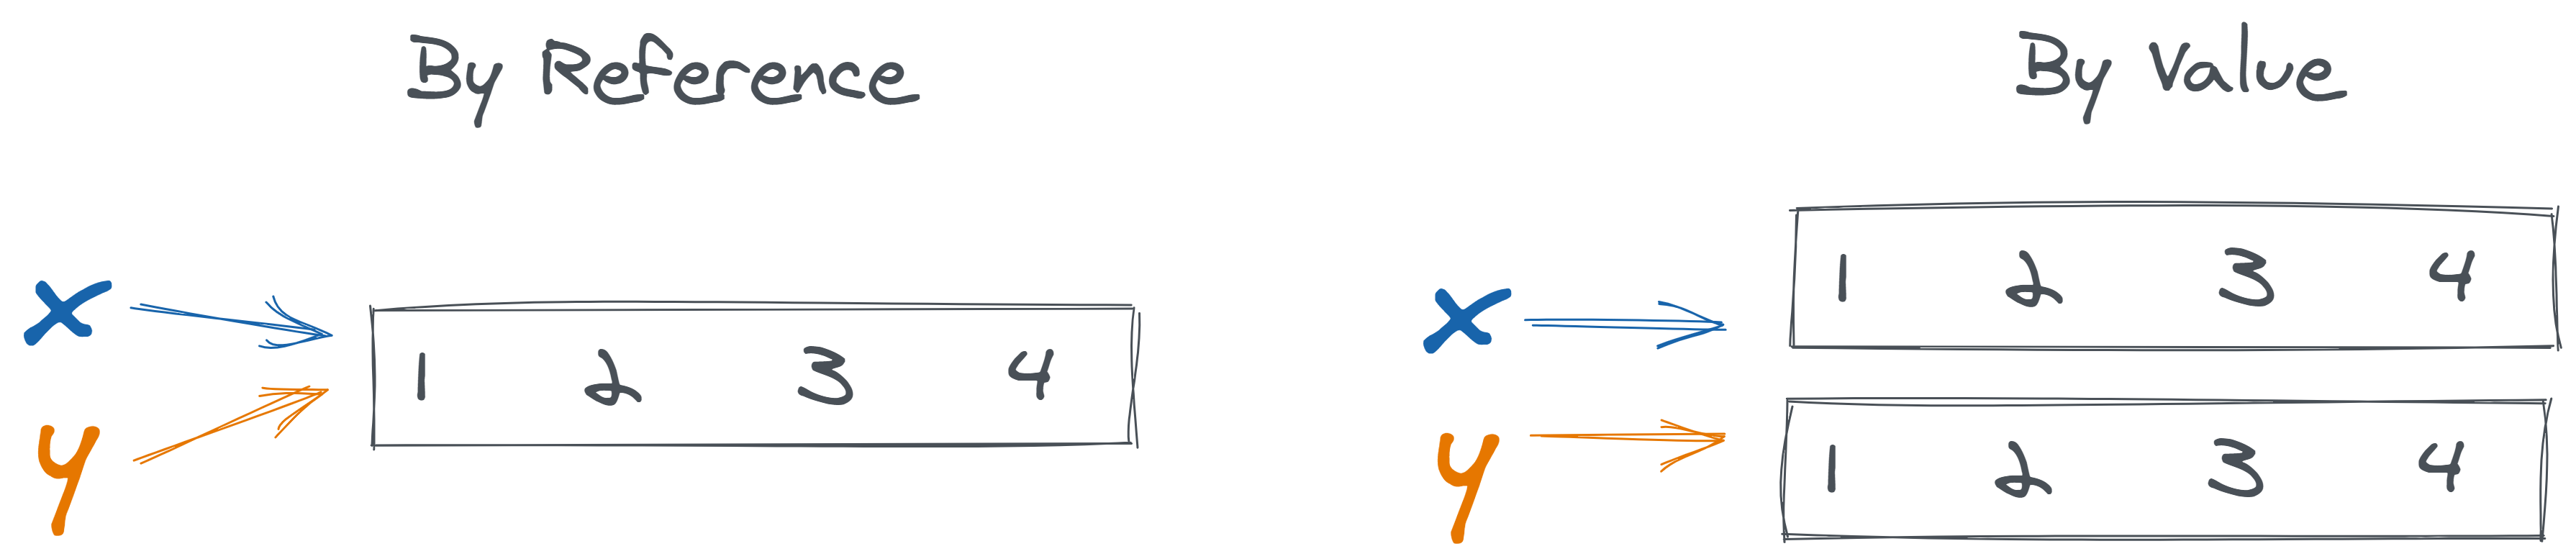
\includegraphics[width=0.9\linewidth]{figures/comp-quan/ref-val} 

}

\caption{Different relationships between named variables and their values}\label{fig:unnamed-chunk-74}
\end{figure}

When might each be preferred?

What risks are there if we don't understand which we are doing?

In Python

\begin{Shaded}
\begin{Highlighting}[]
\NormalTok{x }\OperatorTok{=}\NormalTok{ [}\DecValTok{1}\NormalTok{,}\DecValTok{2}\NormalTok{,}\DecValTok{3}\NormalTok{]}
\NormalTok{y }\OperatorTok{=}\NormalTok{ x}
\NormalTok{y.append(}\DecValTok{4}\NormalTok{)}
\BuiltInTok{print}\NormalTok{(y)}
\BuiltInTok{print}\NormalTok{(x)}
\end{Highlighting}
\end{Shaded}

\begin{verbatim}
## [1, 2, 3, 4]
## [1, 2, 3, 4]
\end{verbatim}

\begin{Shaded}
\begin{Highlighting}[]
\NormalTok{z }\OperatorTok{=}\NormalTok{ x.copy()}
\NormalTok{z.append(}\DecValTok{5}\NormalTok{)}
\BuiltInTok{print}\NormalTok{(z)}
\BuiltInTok{print}\NormalTok{(x)}
\end{Highlighting}
\end{Shaded}

\begin{verbatim}
## [1, 2, 3, 4, 5]
## [1, 2, 3, 4]
\end{verbatim}

pandas DataFrame methods with \texttt{inplace} arg (\texttt{False} is default)

In R

\begin{Shaded}
\begin{Highlighting}[]
\FunctionTok{library}\NormalTok{(data.table)}
\end{Highlighting}
\end{Shaded}

\begin{verbatim}
## 
## Attaching package: 'data.table'
\end{verbatim}

\begin{verbatim}
## The following objects are masked from 'package:dplyr':
## 
##     between, first, last
\end{verbatim}

\begin{Shaded}
\begin{Highlighting}[]
\NormalTok{DT }\OtherTok{\textless{}{-}} \FunctionTok{data.table}\NormalTok{(}\AttributeTok{a=}\FunctionTok{c}\NormalTok{(}\DecValTok{1}\NormalTok{,}\DecValTok{2}\NormalTok{), }\AttributeTok{b=}\FunctionTok{c}\NormalTok{(}\DecValTok{11}\NormalTok{,}\DecValTok{12}\NormalTok{))}
\FunctionTok{print}\NormalTok{(DT)}
\end{Highlighting}
\end{Shaded}

\begin{verbatim}
##    a  b
## 1: 1 11
## 2: 2 12
\end{verbatim}

\begin{Shaded}
\begin{Highlighting}[]
\NormalTok{newDT }\OtherTok{\textless{}{-}}\NormalTok{ DT        }\CommentTok{\# reference, not copy}
\NormalTok{newDT[}\DecValTok{1}\NormalTok{, a }\SpecialCharTok{:}\ErrorTok{=} \DecValTok{100}\NormalTok{] }\CommentTok{\# modify new DT}

\FunctionTok{print}\NormalTok{(DT)          }\CommentTok{\# DT is modified too.}
\end{Highlighting}
\end{Shaded}

\begin{verbatim}
##      a  b
## 1: 100 11
## 2:   2 12
\end{verbatim}

\begin{Shaded}
\begin{Highlighting}[]
\NormalTok{DT }\OtherTok{=} \FunctionTok{data.table}\NormalTok{(}\AttributeTok{a=}\FunctionTok{c}\NormalTok{(}\DecValTok{1}\NormalTok{,}\DecValTok{2}\NormalTok{), }\AttributeTok{b=}\FunctionTok{c}\NormalTok{(}\DecValTok{11}\NormalTok{,}\DecValTok{12}\NormalTok{))}
\NormalTok{newDT }\OtherTok{\textless{}{-}}\NormalTok{ DT        }
\NormalTok{newDT}\SpecialCharTok{$}\NormalTok{b[}\DecValTok{2}\NormalTok{] }\OtherTok{\textless{}{-}} \DecValTok{200}  \CommentTok{\# new operation}
\NormalTok{newDT[}\DecValTok{1}\NormalTok{, a }\SpecialCharTok{:}\ErrorTok{=} \DecValTok{100}\NormalTok{]}

\FunctionTok{print}\NormalTok{(DT)}
\end{Highlighting}
\end{Shaded}

\begin{verbatim}
##    a  b
## 1: 1 11
## 2: 2 12
\end{verbatim}

From \url{https://stackoverflow.com/questions/10225098/understanding-exactly-when-a-data-table-is-a-reference-to-vs-a-copy-of-another}

\hypertarget{trusting-tools}{%
\section{Trusting Tools}\label{trusting-tools}}

\hypertarget{delegating-decisions}{%
\subsection{Delegating decisions}\label{delegating-decisions}}

A theme throughout this book is the fundamentally \emph{social} nature of data analysis. Data analysis is fraught without understanding the countless decisions made along the way by those who generated it (whose data is reflected), those who collected it, those who migrated it, and those who have posed questions of it. On one hand, this is a beautiful aspect of analysis; on the other hand, it means that analysts and their analyses are subject to all of the cognitive and social psychological biases of everyday humans.

One such bias is ``social proof'': assuming that if a tool behaves a certain way, it must be because it is correct.

Assuming that our tools know best is admittedly an attractive proposition. It appeals to a desire to think that someone, somewhere is ``in charge'' and, perhaps more critically, helps us avoid a domino effect of distrust (If we \emph{don't} trust our tools how can we trust our results? And if we can't trust our results, how can we trust anything at all?) Unfortunately, there are many reasons are tools might not know best. For example, the tool's developer might have:

\begin{itemize}
\tightlist
\item
  Made a mistake
\item
  Had a different analysis problem in mind with a different optimal approach
\item
  Been optimizing for a different constraint (e.g.~explainability vs.~accuracy, speed vs.~theoretical properties)
\item
  Come from a community with different norms
\item
  Been affording users the flexibility to do things many ways even if they don't agree
\item
  Built a certain feature for a different purpose than how you are using it
\item
  Not thought about it at all
\end{itemize}

As a few concrete examples from popular open source tools. We'll look briefly at the prominent python library \texttt{scikitlearn} for machine learning and Apache Spark, an engine for large-scale distributed data processing.

\hypertarget{defaults-in-scikitlearn}{%
\subsubsection{\texorpdfstring{Defaults in \texttt{scikitlearn}}{Defaults in scikitlearn}}\label{defaults-in-scikitlearn}}

\texttt{scikitlearn}'s default behavior for logistic regression modeling\footnote{A classic modeling technique for predicting binary (yes/no) outcomes} automatically applies L2 regularization. You might or might not know what this means, and you might or might not want to apply it to your problem. That's fine. The important thing is that it \emph{will} change your estimates and predictions, and it is \emph{not} a part of the classical definition of that algorithm (for modelers coming from a statistical background.)

Of course, there's nothing inherently wrong about this choice; the library authors just had different goals than a typical statistical. \texttt{scikitlearn} developer Olivier Grisel explains \href{https://twitter.com/ogrisel/status/1167438229655773186?s=20}{on Twitter} that this choice (and others in the library) is explained because ``Scikit-learn was always designed to make it easy to get good predictive accuracy (eg as measured by CV) rather than as statistical inference library.'' Additionally, this choice is documented in bold \href{https://scikit-learn.org/stable/modules/generated/sklearn.linear_model.LogisticRegression.html}{in the function documentation}.

However, an analyst could easily miss this nuance if they do not \emph{read} the documentation. Or, if they \emph{misinterpret} this choice as social proof that regularization is always the right approach, they might not make the best choice for their own analysis.

\hypertarget{algorithms-in-spark}{%
\subsubsection{\texorpdfstring{Algorithms in \texttt{Spark}}{Algorithms in Spark}}\label{algorithms-in-spark}}

As a second example, according to a 2015 \href{https://issues.apache.org/jira/browse/SPARK-5133}{Jira ticket}, developers of Spark considered multiple methodologies they could use when adding the functionality to compute feature importance for a random forest. Ultimately, a core contributor advised against permutation importance due to its computational cost.

\begin{figure}

{\centering 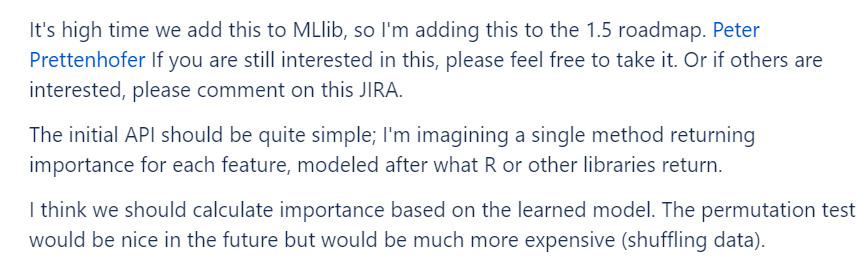
\includegraphics[width=0.9\linewidth]{figures/comp-quan/spark-jira} 

}

\caption{JIRA ticket for Spark with a discussion of which random forest variable importance algorithm to implement}\label{fig:unnamed-chunk-78}
\end{figure}

Clearly, no one wants a workflow that is too costly or timely to run. So, once again, there is no right or wrong. However, since every approach to feature importance has its own biases, pitfalls, and challenges in interpretation, it's a mistake for an end-user to not carefully understand which algorithm is used and why.

\hypertarget{off-label-use-todo}{%
\subsection{``Off-Label'' Use (TODO)}\label{off-label-use-todo}}

coined in \url{https://www.rstudio.com/resources/rstudioglobal-2021/maintaining-the-house-the-tidyverse-built/}

\hypertarget{security-todo}{%
\subsection{Security (TODO)}\label{security-todo}}

namespace squatting

executable code

\hypertarget{inefficient-processing-todo}{%
\section{Inefficient Processing (TODO)}\label{inefficient-processing-todo}}

\hypertarget{strategies-wip}{%
\section{Strategies (WIP)}\label{strategies-wip}}

Paragraph 1 TODO

Some computational quandaries are inherent to our tools themselves, but often they are a function both of the tools and the ways we chose to use them. More strategies related to writing robust and resilient code will be discussed in Chapter \ref{comp-code} (Complexify Code).

\hypertarget{understand-the-intent-1}{%
\subsection{Understand the intent}\label{understand-the-intent-1}}

\begin{itemize}
\tightlist
\item
  read the docs
\item
  look at examples
\end{itemize}

\hypertarget{understand-the-execution-1}{%
\subsection{Understand the execution}\label{understand-the-execution-1}}

\begin{itemize}
\tightlist
\item
  test out simple examples (like we've been doing)
\item
  specificlly try out corner cases
\end{itemize}

\hypertarget{be-explicit-not-implicit}{%
\subsection{Be explicit not implicit}\label{be-explicit-not-implicit}}

\begin{itemize}
\tightlist
\item
  default arguments
\item
  examples above with casting, coalescing
\end{itemize}

\hypertarget{real-world-disasters-wip}{%
\section{Real World Disasters (WIP)}\label{real-world-disasters-wip}}

\url{https://www.theguardian.com/politics/2020/oct/05/how-excel-may-have-caused-loss-of-16000-covid-tests-in-england}

\begin{quote}
The data error, which led to 15,841 positive tests being left off the official daily figures, means than 50,000 potentially infectious people may have been missed by contact tracers and not told to self-isolate.
\end{quote}

\hypertarget{part-analysis}{%
\part*{Analysis}\label{part-analysis}}


\hypertarget{eg-agg}{%
\chapter{Egregious Aggregations (WIP)}\label{eg-agg}}

Once armed with an understanding of the data and tools available for analysis, a common start to analysis is exploring data with \emph{aggregation}.
At its heart, any sort of data analysis is the process of condensing raw data into something more manageable and useful while giving up as little of the information as possible.

Many elementary tools for this task are much better at the comprehension task than the preservation one.
We learn rigorous assumptions to consider and validate when studying linear regression, but basic arithmetic aggregation presents itself as agnostic and welcome to any type of data.
However, the underlying distributions of our variables and the relationships between them have a significant impact on the how informative and interpretable various summarizations are.

In this chapter, we will explore different ways that univariate and multivariate aggregations can be naive or uninformative.

\hypertarget{similar-in-summary}{%
\section{Similar in Summary}\label{similar-in-summary}}

Anscombe's Quartet

The datasaurus dozen \citep{datasaurus} and the \texttt{datasauRus} R package \citep{R-datasauRus}

\begin{Shaded}
\begin{Highlighting}[]
\FunctionTok{library}\NormalTok{(datasauRus)}
\end{Highlighting}
\end{Shaded}

\begin{Shaded}
\begin{Highlighting}[]
\NormalTok{df }\OtherTok{\textless{}{-}}\NormalTok{ datasauRus}\SpecialCharTok{::}\NormalTok{datasaurus\_dozen}
\FunctionTok{head}\NormalTok{(df)}
\end{Highlighting}
\end{Shaded}

\begin{verbatim}
## # A tibble: 6 x 3
##   dataset     x     y
##   <chr>   <dbl> <dbl>
## 1 dino     55.4  97.2
## 2 dino     51.5  96.0
## 3 dino     46.2  94.5
## 4 dino     42.8  91.4
## 5 dino     40.8  88.3
## 6 dino     38.7  84.9
\end{verbatim}

\begin{table}

\caption{\label{tab:datasaurus-tbl}Summary statistics for Datasaurus Dozen datasets}
\centering
\begin{tabular}[t]{l|r|r|r|r|r}
\hline
dataset & mean(x) & mean(y) & var(x) & var(y) & cor(x, y)\\
\hline
away & 54.27 & 47.84 & 281.2 & 725.8 & -0.064\\
\hline
bullseye & 54.27 & 47.83 & 281.2 & 725.5 & -0.069\\
\hline
circle & 54.27 & 47.84 & 280.9 & 725.2 & -0.068\\
\hline
dino & 54.26 & 47.83 & 281.1 & 725.5 & -0.064\\
\hline
dots & 54.26 & 47.84 & 281.2 & 725.2 & -0.060\\
\hline
h\_lines & 54.26 & 47.83 & 281.1 & 725.8 & -0.062\\
\hline
high\_lines & 54.27 & 47.84 & 281.1 & 725.8 & -0.069\\
\hline
slant\_down & 54.27 & 47.84 & 281.1 & 725.6 & -0.069\\
\hline
slant\_up & 54.27 & 47.83 & 281.2 & 725.7 & -0.069\\
\hline
star & 54.27 & 47.84 & 281.2 & 725.2 & -0.063\\
\hline
v\_lines & 54.27 & 47.84 & 281.2 & 725.6 & -0.069\\
\hline
wide\_lines & 54.27 & 47.83 & 281.2 & 725.7 & -0.067\\
\hline
x\_shape & 54.26 & 47.84 & 281.2 & 725.2 & -0.066\\
\hline
\end{tabular}
\end{table}

\begin{figure}
\centering
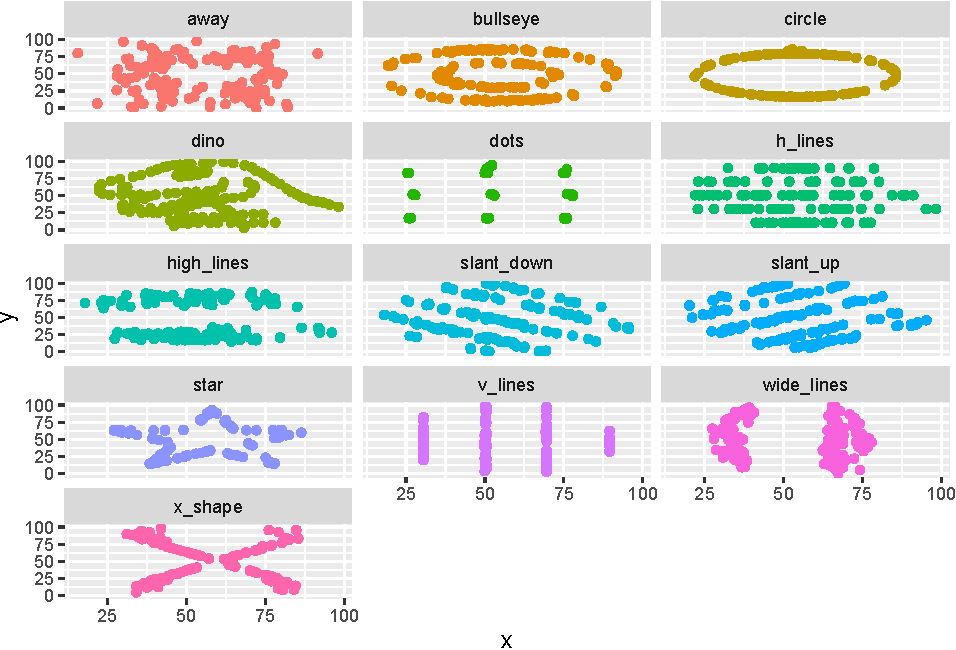
\includegraphics{bookdown_files/figure-latex/datasaurus-plot-1.pdf}
\caption{\label{fig:datasaurus-plot}Scatterplots for Datasaurus Dozen datasets}
\end{figure}

While this is clearly a contrived example (and, if you so chose to check out the paper, a very cleverly contrived example!), its also a cautionary tale. Summary statistics are not just insufficient when they focus on central tendency (e.g.~mean) instead of spread. In this example, even an examination of variation and covariation led to an overly simplistic view of the underlying data.

\hypertarget{averages}{%
\section{Averages}\label{averages}}

\hypertarget{averaging-skewed-data}{%
\subsection{Averaging skewed data}\label{averaging-skewed-data}}

Arithmetic average versus colloquial meaning of average as ``typical''

Skewed data

Multimodal data / mixture models

\hypertarget{no-average-observation}{%
\subsection{No ``average'' observation}\label{no-average-observation}}

In the previous section, the average represented a point in the relevant data \emph{range} even if it was not perhaps the one most representative of a ``typical'' observation.
We discussed how in some situations this quantity may be a reasonable answer to certain types of questions and an aid for certain types of decisions.

However, when we seek an average \emph{profile} over multiple variables, the problems of averages are further compounded.
We may end up with a set of ``average'' summary statistics that are not representative of any part of our population.

To see this, let's assume we are working with data for a company with a subscription business model.
We might be interested in profiling the age of each account (how long they have been a subscriber) and their activity (measured by amount spent on an e-commerce platform, files downloaded on a streaming service, etc.)

The following code simulates a set of observations:
80\% of accounts are between 0 to 3 years in age and have an average activity level of 100 while 20\% of accounts are older than 3 years in age and have an average activity level of 500.
(Don't over-think the specific probability distributions lived here.
We are concerned with interrogating the properties of the average and not with simulating a realistic data generating process.
Giving ourselves permission to be wrong or ``lazy'' about unimportant things gives us more energy to focus on what matters.)

\begin{Shaded}
\begin{Highlighting}[]
\FunctionTok{set.seed}\NormalTok{(}\DecValTok{123}\NormalTok{)}

\CommentTok{\# define simulation parameters {-}{-}{-}{-}}
\DocumentationTok{\#\# n: total observations}
\DocumentationTok{\#\# p: proportion of observations in group 1}
\NormalTok{n }\OtherTok{\textless{}{-}} \DecValTok{5000}
\NormalTok{p }\OtherTok{\textless{}{-}} \FloatTok{0.8}
\NormalTok{n1 }\OtherTok{\textless{}{-}}\NormalTok{ n}\SpecialCharTok{*}\NormalTok{p}
\NormalTok{n2 }\OtherTok{\textless{}{-}}\NormalTok{ n}\SpecialCharTok{*}\NormalTok{(}\DecValTok{1}\SpecialCharTok{{-}}\NormalTok{p)}

\CommentTok{\# generate fake dataset with two groups {-}{-}{-}{-}}
\NormalTok{df }\OtherTok{\textless{}{-}} 
  \FunctionTok{data.frame}\NormalTok{(}
    \AttributeTok{age =} \FunctionTok{c}\NormalTok{(}\FunctionTok{runif}\NormalTok{(n1,   }\DecValTok{0}\NormalTok{,  }\DecValTok{3}\NormalTok{), }\FunctionTok{runif}\NormalTok{(n2,   }\DecValTok{3}\NormalTok{, }\DecValTok{10}\NormalTok{)),}
    \AttributeTok{act =} \FunctionTok{c}\NormalTok{(}\FunctionTok{rnorm}\NormalTok{(n1, }\DecValTok{100}\NormalTok{, }\DecValTok{10}\NormalTok{), }\FunctionTok{rnorm}\NormalTok{(n2, }\DecValTok{500}\NormalTok{, }\DecValTok{10}\NormalTok{))}
\NormalTok{  )}
\end{Highlighting}
\end{Shaded}

Figure \ref{fig:multivar-avg} shows a scatterplot of the relationship between account age (x-axis) and activity level (y-axis).
Meanwhile, the marginal rug plots shows the univariate distribution of each variable.
The sole red dot denotes the coordinates of the average age and average activity.
Notably, this dot exists in a region of ``zero density'';
that is, it is not representative of \emph{any} customer.
Strategic decisions made with this sort of observation in mind as the ``typical'' might not be destined for success.

\begin{figure}
\centering
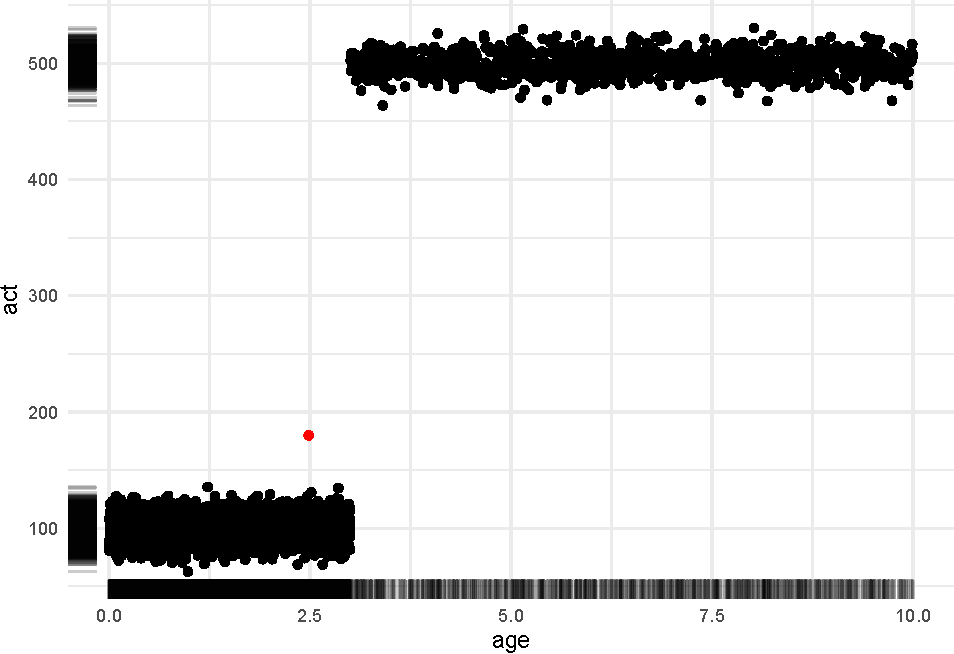
\includegraphics{bookdown_files/figure-latex/multivar-avg-1.pdf}
\caption{\label{fig:multivar-avg}A scatterplot of two variables and their averages}
\end{figure}

\hypertarget{the-product-of-averages}{%
\subsection{The product of averages}\label{the-product-of-averages}}

As the above example shows, averages of multivariate data can produce poor summaries -- particularly when these variables are interrelated\footnote{We intentionally avoid the word \emph{correlated} here to emphasize the fact that \emph{correlation} refers more strictly to linear relationships}.

A second implication of this observation is that deriving additional computations based on pre-averaged numbers is likely to obtain inaccurate results.

For example, consider that we wish to estimate the average dollar amount of returns per any e-commerce order.
Orders may generally be a mixture of low-price orders (around \$50 on average) and high-price orders (around \$250 on average).
Low-price orders may have a 10\% probability of being returned while high price orders have a 20\% probability.
(Again, are these numbers, distributions, or relationships hyper-realistic?
Not at all.
However, once again we are telling ourselves a story just to reason about numerical properties, so we have to give ourselves permission to not focus on irrelevant details.)

\begin{Shaded}
\begin{Highlighting}[]
\FunctionTok{set.seed}\NormalTok{(}\DecValTok{123}\NormalTok{)}

\CommentTok{\# define simulation parameters {-}{-}{-}{-}}
\DocumentationTok{\#\# n: observations per group}
\DocumentationTok{\#\# pr[1|2]: mean price per group}
\NormalTok{n }\OtherTok{\textless{}{-}} \DecValTok{100}
\NormalTok{pr1 }\OtherTok{\textless{}{-}} \DecValTok{50}
\NormalTok{pr2 }\OtherTok{\textless{}{-}} \DecValTok{250}
\NormalTok{pr\_sd }\OtherTok{\textless{}{-}} \DecValTok{5}
\NormalTok{re1 }\OtherTok{\textless{}{-}} \FloatTok{0.1}
\NormalTok{re2 }\OtherTok{\textless{}{-}} \FloatTok{0.2}

\CommentTok{\# simulate spend amounts and return indicators {-}{-}{-}{-}}
\NormalTok{amt\_spend  }\OtherTok{\textless{}{-}} \FunctionTok{c}\NormalTok{(}\FunctionTok{rnorm}\NormalTok{(n, pr1, pr\_sd), }\FunctionTok{rnorm}\NormalTok{(n, pr2, pr\_sd))}
\NormalTok{ind\_return }\OtherTok{\textless{}{-}} \FunctionTok{c}\NormalTok{(}\FunctionTok{rbinom}\NormalTok{(n, }\DecValTok{1}\NormalTok{, re1),    }\FunctionTok{rbinom}\NormalTok{(n, }\DecValTok{1}\NormalTok{, re2))}

\CommentTok{\# compute summary statistics {-}{-}{-}{-}}
\NormalTok{average\_of\_product }\OtherTok{\textless{}{-}} \FunctionTok{mean}\NormalTok{(amt\_spend }\SpecialCharTok{*}\NormalTok{ ind\_return)}
\NormalTok{product\_of\_average }\OtherTok{\textless{}{-}} \FunctionTok{mean}\NormalTok{(amt\_spend) }\SpecialCharTok{*} \FunctionTok{mean}\NormalTok{(ind\_return)}
\end{Highlighting}
\end{Shaded}

The \emph{true} average amount returned across all of our orders is 36.0438 (from the \texttt{average\_of\_product} variable).
However, if instead we already knew an average spend amount and an average return proportion, we might be inclined to compute the \texttt{product\_of\_average} method which returns a value of 26.9923.
(This is a difference of 9.05 relative to an average purchase amount of 150.)

At first, this may seem unintuitive until we write out the formulas and realize that these metrics are, in fact, two very different quantities:

\[ \frac{ \sum_{1}^{n} Spend }{\sum_{1}^{n} 1} \ * \frac{ \sum_{1}^{n} I(Return) }{\sum_{1}^{n} 1} \] over all \(n\) orders

versus

\[ \frac{\sum_{1}^{n} Spend * I(Return)}{\sum_{1}^{n} 1} \]

If this still feels counterintuitive, we can see how much of the difference is accounted for by the interrelation between our two variables.
In the following code, we break the relationship between the variables by randomly reordering the \texttt{ind\_return} variable so it is no longer has any true relationship to the corresponding \texttt{amt\_spend} variable.

\begin{Shaded}
\begin{Highlighting}[]
\CommentTok{\# randomly reorder one of two variables to break relationships {-}{-}{-}{-}}
\NormalTok{ind\_return }\OtherTok{\textless{}{-}} \FunctionTok{sample}\NormalTok{(ind\_return, }\AttributeTok{size =} \DecValTok{200}\NormalTok{)}

\CommentTok{\# recompute variables {-}{-}{-}{-}}
\NormalTok{average\_of\_product }\OtherTok{\textless{}{-}} \FunctionTok{mean}\NormalTok{(amt\_spend }\SpecialCharTok{*}\NormalTok{ ind\_return)}
\NormalTok{product\_of\_average }\OtherTok{\textless{}{-}} \FunctionTok{mean}\NormalTok{(amt\_spend) }\SpecialCharTok{*} \FunctionTok{mean}\NormalTok{(ind\_return)}
\end{Highlighting}
\end{Shaded}

After redoing the calculations, we find that th two values are much closer.
\texttt{average\_of\_product} is now 24.1041 and \texttt{product\_of\_average} is now 26.9923.
These are notably still not the same number so that does not mean that these two equations are equivalent if variables are unrelated;
however, this second result once again illustrates the extent to which interrelations can defy our naive intuitions.

\hypertarget{ratios}{%
\section{Ratios}\label{ratios}}

\hypertarget{picking-the-right-denominator}{%
\subsection{Picking the right denominator}\label{picking-the-right-denominator}}

\hypertarget{sample-size-effects}{%
\subsection{Sample size effects}\label{sample-size-effects}}

\hypertarget{trends}{%
\section{Trends}\label{trends}}

\hypertarget{if-trends-continue}{%
\subsection{\texorpdfstring{``If trends continue\ldots{}''}{``If trends continue\ldots''}}\label{if-trends-continue}}

\hypertarget{seasonality}{%
\subsection{Seasonality}\label{seasonality}}

\hypertarget{strategies-todo-1}{%
\section{Strategies (TODO)}\label{strategies-todo-1}}

\hypertarget{real-world-disasters-todo}{%
\section{Real World Disasters (TODO)}\label{real-world-disasters-todo}}

Straight vs weighted averages in COVID positivity rates \citep{indy_rates}

\begin{quote}
The changes could result in real-world differences for Hoosiers, because the state uses a county's positivity rate as one of the numbers to determine which restrictions that county will face. Those restrictions determine how many people may gather, among other items.
\end{quote}

\begin{quote}
Some Hoosiers may see loosened restrictions because of the changes. While Box said the county-level impact will be mixed, she predicted some smaller counties will see a decline in positivity rate after the changes.
\end{quote}

\begin{quote}
``The change to the methodology is how we calculate the seven-day positivity rate for counties. In the past, similar to many states, we've added each day's positivity rate for seven days and divided by seven to obtain the week's positivity rate. Now we will add all of the positive tests for the week and divide by the total tests done that week to determine the week's positivity rate. This will help to minimize the effect that a high variability in the number of tests done each day can have on the week's overall positivity, especially for our smaller counties.''
\end{quote}

\begin{Shaded}
\begin{Highlighting}[]
\NormalTok{avg\_of\_ratios }\OtherTok{\textless{}{-}}\NormalTok{ (}\DecValTok{10}\SpecialCharTok{/}\DecValTok{100} \SpecialCharTok{+} \DecValTok{90}\SpecialCharTok{/}\DecValTok{100}\NormalTok{) }\SpecialCharTok{/} \DecValTok{2}

\NormalTok{ratio\_of\_sums }\OtherTok{\textless{}{-}}\NormalTok{ (}\DecValTok{10} \SpecialCharTok{+} \DecValTok{90}\NormalTok{) }\SpecialCharTok{/}\NormalTok{ (}\DecValTok{100} \SpecialCharTok{+} \DecValTok{100}\NormalTok{)}

\NormalTok{avg\_of\_ratios }\SpecialCharTok{==}\NormalTok{ ratio\_of\_sums}
\end{Highlighting}
\end{Shaded}

\begin{verbatim}
## [1] TRUE
\end{verbatim}

\begin{Shaded}
\begin{Highlighting}[]
\NormalTok{avg\_of\_ratios\_uneq }\OtherTok{\textless{}{-}}\NormalTok{ (}\DecValTok{10}\SpecialCharTok{/}\DecValTok{100} \SpecialCharTok{+} \DecValTok{180} \SpecialCharTok{/} \DecValTok{200}\NormalTok{) }\SpecialCharTok{/} \DecValTok{2}

\NormalTok{ratio\_of\_sums\_uneq }\OtherTok{\textless{}{-}}\NormalTok{ (}\DecValTok{10} \SpecialCharTok{+} \DecValTok{180}\NormalTok{) }\SpecialCharTok{/}\NormalTok{ (}\DecValTok{100} \SpecialCharTok{+} \DecValTok{200}\NormalTok{)}

\NormalTok{avg\_of\_ratios\_uneq }\SpecialCharTok{==}\NormalTok{ ratio\_of\_sums\_uneq}
\end{Highlighting}
\end{Shaded}

\begin{verbatim}
## [1] FALSE
\end{verbatim}

\begin{Shaded}
\begin{Highlighting}[]
\NormalTok{weightavg\_of\_ratios\_uneq }\OtherTok{\textless{}{-}}\NormalTok{ (}\DecValTok{100}\SpecialCharTok{/}\DecValTok{300}\NormalTok{)}\SpecialCharTok{*}\NormalTok{(}\DecValTok{10}\SpecialCharTok{/}\DecValTok{100}\NormalTok{) }\SpecialCharTok{+}\NormalTok{ (}\DecValTok{200}\SpecialCharTok{/}\DecValTok{300}\NormalTok{)}\SpecialCharTok{*}\NormalTok{(}\DecValTok{180}\SpecialCharTok{/}\DecValTok{200}\NormalTok{)}

\NormalTok{ratio\_of\_sums\_uneq }\SpecialCharTok{==}\NormalTok{ weightavg\_of\_ratios\_uneq}
\end{Highlighting}
\end{Shaded}

\begin{verbatim}
## [1] TRUE
\end{verbatim}

Recall that the standard deviation of sample proportion is \(\sqrt(p*(1-p)/n)\)

link to discussions of sample size and different types of averages

\begin{Shaded}
\begin{Highlighting}[]
\FunctionTok{set.seed}\NormalTok{(}\DecValTok{123}\NormalTok{)}

\CommentTok{\# define simulation parameters {-}{-}{-}{-}}
\DocumentationTok{\#\# n: total draws from binomial distribution}
\DocumentationTok{\#\# p: proportion of successes}
\NormalTok{p }\OtherTok{\textless{}{-}} \FloatTok{0.5}
\NormalTok{n }\OtherTok{\textless{}{-}} \DecValTok{1000}

\CommentTok{\# sample from binomials of different size {-}{-}{-}{-}}
\NormalTok{s010 }\OtherTok{\textless{}{-}} \FunctionTok{rbinom}\NormalTok{(n,  }\DecValTok{10}\NormalTok{, p) }\SpecialCharTok{/}  \DecValTok{10}
\NormalTok{s100 }\OtherTok{\textless{}{-}} \FunctionTok{rbinom}\NormalTok{(n, }\DecValTok{100}\NormalTok{, p) }\SpecialCharTok{/} \DecValTok{100}
\NormalTok{s500 }\OtherTok{\textless{}{-}} \FunctionTok{rbinom}\NormalTok{(n, }\DecValTok{500}\NormalTok{, p) }\SpecialCharTok{/} \DecValTok{500}

\CommentTok{\# set results as dataframe for inspection {-}{-}{-}{-}}
\NormalTok{df }\OtherTok{\textless{}{-}} \FunctionTok{data.frame}\NormalTok{(}
  \AttributeTok{s =} \FunctionTok{rep}\NormalTok{(}\FunctionTok{c}\NormalTok{(}\DecValTok{10}\NormalTok{, }\DecValTok{100}\NormalTok{, }\DecValTok{500}\NormalTok{), }\AttributeTok{each =}\NormalTok{ n),}
  \AttributeTok{x =} \FunctionTok{c}\NormalTok{(s010, s100, s500)}
\NormalTok{)}
\end{Highlighting}
\end{Shaded}

\begin{Shaded}
\begin{Highlighting}[]
\FunctionTok{library}\NormalTok{(ggplot2)}

\FunctionTok{ggplot}\NormalTok{(}\AttributeTok{data =}\NormalTok{ df) }\SpecialCharTok{+}
  \FunctionTok{aes}\NormalTok{(}\AttributeTok{x =}\NormalTok{ x, }\AttributeTok{col =} \FunctionTok{as.character}\NormalTok{(s)) }\SpecialCharTok{+}
  \FunctionTok{geom\_density}\NormalTok{() }\SpecialCharTok{+}
  \FunctionTok{geom\_vline}\NormalTok{(}\AttributeTok{xintercept =}\NormalTok{ p, }\AttributeTok{col =} \StringTok{\textquotesingle{}darkgrey\textquotesingle{}}\NormalTok{, }\AttributeTok{linetype =} \DecValTok{2}\NormalTok{) }\SpecialCharTok{+}
  \FunctionTok{labs}\NormalTok{(}
    \AttributeTok{title =} \StringTok{"Sampling Distribution for p = 0.5"}\NormalTok{,}
    \AttributeTok{col =} \StringTok{"Sample Size"}
\NormalTok{  ) }\SpecialCharTok{+}
  \FunctionTok{scale\_x\_continuous}\NormalTok{(}\AttributeTok{breaks =} \FunctionTok{seq}\NormalTok{(}\DecValTok{0}\NormalTok{, }\DecValTok{1}\NormalTok{, }\FloatTok{0.1}\NormalTok{), }\AttributeTok{labels =} \FunctionTok{seq}\NormalTok{(}\DecValTok{0}\NormalTok{, }\DecValTok{1}\NormalTok{, }\FloatTok{0.1}\NormalTok{)) }\SpecialCharTok{+}
  \FunctionTok{theme}\NormalTok{(}
    \AttributeTok{plot.title =} \FunctionTok{element\_text}\NormalTok{(}\AttributeTok{hjust =} \FloatTok{0.5}\NormalTok{),}
    \AttributeTok{legend.position =} \StringTok{"bottom"}
\NormalTok{  )}
\end{Highlighting}
\end{Shaded}

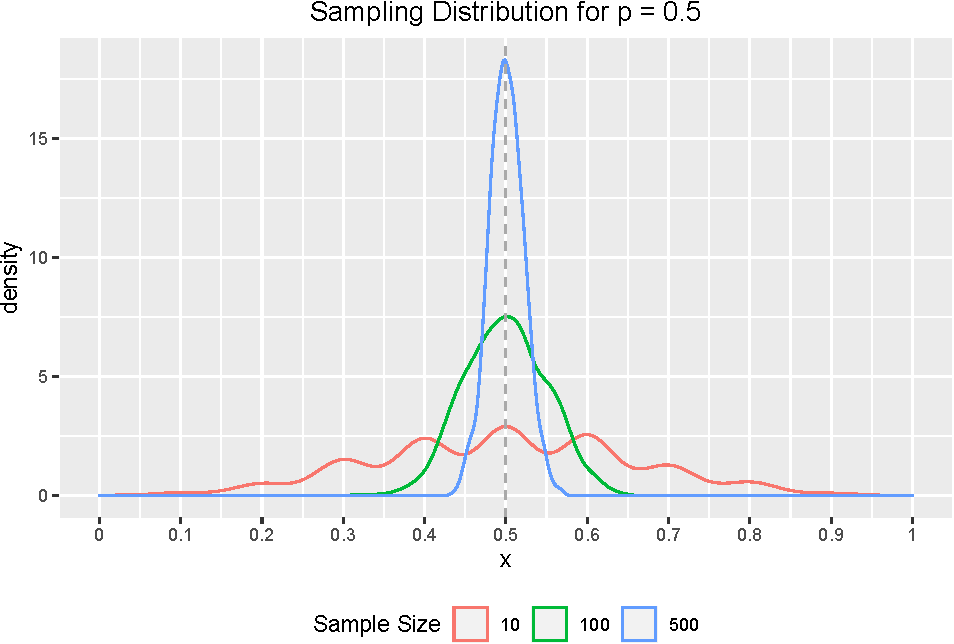
\includegraphics{bookdown_files/figure-latex/unnamed-chunk-123-1.pdf}

\hypertarget{vex-viz}{%
\chapter{Vexing Visualization (TODO)}\label{vex-viz}}

\hypertarget{incr-infe}{%
\chapter{Incredible Inferences (TODO)}\label{incr-infe}}

Previously, we have seen how different inputs like data, tools, and methods can add risks to our data analysis. However, the battle is not won simply when we get our first set of \emph{outputs}. In this chapter, we will explore common errors in interpreting the results of our analysis by exploring aspects of bias, missingness, and confounding.

\hypertarget{feature-leakage}{%
\section{Feature Leakage}\label{feature-leakage}}

\begin{Shaded}
\begin{Highlighting}[]
\NormalTok{n }\OtherTok{\textless{}{-}} \DecValTok{1000}
\NormalTok{minutes\_month1 }\OtherTok{\textless{}{-}} \FunctionTok{runif}\NormalTok{(n, }\DecValTok{60}\NormalTok{, }\DecValTok{1200}\NormalTok{)}
\NormalTok{minutes\_month2 }\OtherTok{\textless{}{-}} \FunctionTok{runif}\NormalTok{(n, }\DecValTok{60}\NormalTok{, }\DecValTok{1200}\NormalTok{) }
\NormalTok{minutes\_tot }\OtherTok{\textless{}{-}}\NormalTok{ minutes\_month1 }\SpecialCharTok{+}\NormalTok{ minutes\_month2}
\NormalTok{df }\OtherTok{\textless{}{-}} \FunctionTok{data.frame}\NormalTok{(minutes\_month1, minutes\_month2, minutes\_tot)}
\end{Highlighting}
\end{Shaded}

Figure \ref{fig:sep-sum} shows\ldots{}

\begin{figure}

{\centering 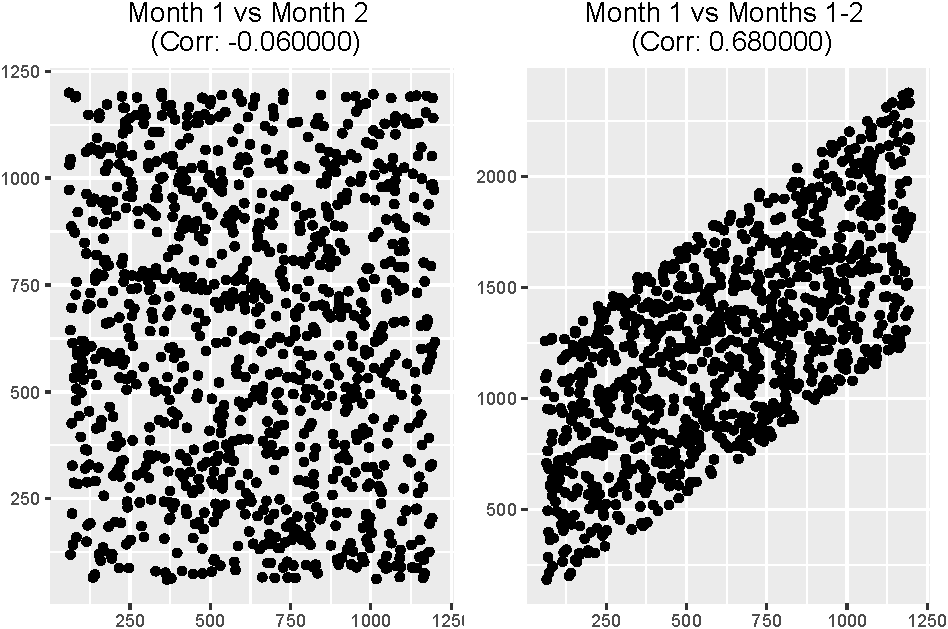
\includegraphics[width=0.9\linewidth]{bookdown_files/figure-latex/sep-sum-1} 

}

\caption{Correlation of idependent versus cumulative quantities}\label{fig:sep-sum}
\end{figure}

\hypertarget{cava-caus}{%
\chapter{Cavalier Causality (TODO)}\label{cava-caus}}

In Chapter \ref{incr-infe} (Incredible Inferences), we began to see that we can be tricked by biases when we lack \emph{causal} thinking and an underlying theory for the data generating process. In this chapter, we will revisit some of these same disasters and introduce some specific frameworks to help us more rigorously explore our analysis for errors and biases and, even better, strategize the best ways to fix them.

\hypertarget{mind-mod}{%
\chapter{Mindless Modeling (TODO)}\label{mind-mod}}

\hypertarget{features}{%
\section{Features}\label{features}}

\hypertarget{targets}{%
\section{Targets}\label{targets}}

\hypertarget{evaluation-metrics}{%
\section{Evaluation Metrics}\label{evaluation-metrics}}

\hypertarget{unsupervised-learning}{%
\section{Unsupervised Learning}\label{unsupervised-learning}}

\hypertarget{lifecycle-management}{%
\section{Lifecycle Management}\label{lifecycle-management}}

\hypertarget{fair-and-ethical-modeling}{%
\section{Fair and Ethical Modeling}\label{fair-and-ethical-modeling}}

\hypertarget{alt-alg}{%
\chapter{Alternative Algorithms (TODO)}\label{alt-alg}}

As the consummate showman, P.T. Barnum is often quoted as saying ``Leave them wanting more''. Unfortunately, statistics professors have less of a flare for drama. Introductory statistics courses will typically introduce a few types of models (for example, linear and \emph{perhaps} logistic regression), and that's a wrap. It's often until students start \emph{taking} the subsequent courses that they are exposed to the true limitations of previous techniques and taught to demand more.

This chapter attempts to flip that paradigm by briefly surveying a broad number of modeling techniques. The goal is not to go into all of the rigorous deals that one should understand to use these models. Instead, we hope to build a ``mental toolbox'' of techniques so that you know where to focus your study when you encounter a problem in the real world.

\hypertarget{not-modeling}{%
\section{Not Modeling}\label{not-modeling}}

\hypertarget{first-principles}{%
\subsection{First Principles}\label{first-principles}}

\hypertarget{simple-analyses}{%
\subsection{Simple Analyses}\label{simple-analyses}}

\hypertarget{extending-linear-regression}{%
\section{Extending Linear Regression}\label{extending-linear-regression}}

\hypertarget{modeling-binary-outcomes}{%
\subsection{Modeling Binary Outcomes}\label{modeling-binary-outcomes}}

\hypertarget{modeling-counts}{%
\subsection{Modeling Counts}\label{modeling-counts}}

\hypertarget{modeling-time-until-an-event}{%
\subsection{Modeling Time Until an Event}\label{modeling-time-until-an-event}}

\hypertarget{modeling-repeated-measures-on-a-population}{%
\subsection{Modeling Repeated Measures on a Population}\label{modeling-repeated-measures-on-a-population}}

\hypertarget{modeling-observations-in-a-nested-hierarchy}{%
\subsection{Modeling Observations in a Nested Hierarchy}\label{modeling-observations-in-a-nested-hierarchy}}

\hypertarget{causal-analysis-patterns}{%
\section{Causal Analysis Patterns}\label{causal-analysis-patterns}}

Similar to \url{https://emilyriederer.netlify.app/post/causal-design-patterns/}

\hypertarget{special-data-types}{%
\section{Special Data Types}\label{special-data-types}}

\hypertarget{duration-analysis}{%
\subsection{Duration Analysis}\label{duration-analysis}}

\hypertarget{time-space-data}{%
\subsection{Time \& Space Data}\label{time-space-data}}

\hypertarget{bayesian-methods}{%
\section{Bayesian Methods}\label{bayesian-methods}}

\hypertarget{simulation-methods}{%
\section{Simulation Methods}\label{simulation-methods}}

\hypertarget{agent-based}{%
\subsection{Agent-Based}\label{agent-based}}

\hypertarget{discrete-event}{%
\subsection{Discrete Event}\label{discrete-event}}

\hypertarget{clustering-beyond-k-means}{%
\section{Clustering (beyond K-Means)}\label{clustering-beyond-k-means}}

\hypertarget{density-based}{%
\subsection{Density-Based}\label{density-based}}

\hypertarget{mixture-models}{%
\subsection{Mixture Models}\label{mixture-models}}

\hypertarget{part-workflow}{%
\part*{Workflow}\label{part-workflow}}


\hypertarget{futi-find}{%
\chapter{Futile Findings (TODO)}\label{futi-find}}

\hypertarget{comp-code}{%
\chapter{Complexifying Code (TODO)}\label{comp-code}}

\hypertarget{reje-repr}{%
\chapter{Rejecting Reproducibility (TODO)}\label{reje-repr}}

``Good Enough Practices in Computational Reproducibility'' \citep{wilson_bryan_cranston_kitzes_nederbragt_teal_2017}

Package managment \citep{R-renv}

environment management

\cleardoublepage

\hypertarget{appendix-appendix}{%
\appendix \addcontentsline{toc}{chapter}{\appendixname}}


\hypertarget{useful-data-generation-functions-todo}{%
\chapter{Useful Data Generation Functions (TODO)}\label{useful-data-generation-functions-todo}}

\hypertarget{common-probability-distributions-todo}{%
\chapter{Common Probability Distributions (TODO)}\label{common-probability-distributions-todo}}

  \bibliography{book.bib,packages.bib}

\backmatter
\printindex

\end{document}
